% Options for packages loaded elsewhere
\PassOptionsToPackage{unicode}{hyperref}
\PassOptionsToPackage{hyphens}{url}
%
\documentclass[
]{book}
\usepackage{amsmath,amssymb}
\usepackage{lmodern}
\usepackage{iftex}
\ifPDFTeX
  \usepackage[T1]{fontenc}
  \usepackage[utf8]{inputenc}
  \usepackage{textcomp} % provide euro and other symbols
\else % if luatex or xetex
  \usepackage{unicode-math}
  \defaultfontfeatures{Scale=MatchLowercase}
  \defaultfontfeatures[\rmfamily]{Ligatures=TeX,Scale=1}
\fi
% Use upquote if available, for straight quotes in verbatim environments
\IfFileExists{upquote.sty}{\usepackage{upquote}}{}
\IfFileExists{microtype.sty}{% use microtype if available
  \usepackage[]{microtype}
  \UseMicrotypeSet[protrusion]{basicmath} % disable protrusion for tt fonts
}{}
\makeatletter
\@ifundefined{KOMAClassName}{% if non-KOMA class
  \IfFileExists{parskip.sty}{%
    \usepackage{parskip}
  }{% else
    \setlength{\parindent}{0pt}
    \setlength{\parskip}{6pt plus 2pt minus 1pt}}
}{% if KOMA class
  \KOMAoptions{parskip=half}}
\makeatother
\usepackage{xcolor}
\usepackage{color}
\usepackage{fancyvrb}
\newcommand{\VerbBar}{|}
\newcommand{\VERB}{\Verb[commandchars=\\\{\}]}
\DefineVerbatimEnvironment{Highlighting}{Verbatim}{commandchars=\\\{\}}
% Add ',fontsize=\small' for more characters per line
\usepackage{framed}
\definecolor{shadecolor}{RGB}{248,248,248}
\newenvironment{Shaded}{\begin{snugshade}}{\end{snugshade}}
\newcommand{\AlertTok}[1]{\textcolor[rgb]{0.94,0.16,0.16}{#1}}
\newcommand{\AnnotationTok}[1]{\textcolor[rgb]{0.56,0.35,0.01}{\textbf{\textit{#1}}}}
\newcommand{\AttributeTok}[1]{\textcolor[rgb]{0.77,0.63,0.00}{#1}}
\newcommand{\BaseNTok}[1]{\textcolor[rgb]{0.00,0.00,0.81}{#1}}
\newcommand{\BuiltInTok}[1]{#1}
\newcommand{\CharTok}[1]{\textcolor[rgb]{0.31,0.60,0.02}{#1}}
\newcommand{\CommentTok}[1]{\textcolor[rgb]{0.56,0.35,0.01}{\textit{#1}}}
\newcommand{\CommentVarTok}[1]{\textcolor[rgb]{0.56,0.35,0.01}{\textbf{\textit{#1}}}}
\newcommand{\ConstantTok}[1]{\textcolor[rgb]{0.00,0.00,0.00}{#1}}
\newcommand{\ControlFlowTok}[1]{\textcolor[rgb]{0.13,0.29,0.53}{\textbf{#1}}}
\newcommand{\DataTypeTok}[1]{\textcolor[rgb]{0.13,0.29,0.53}{#1}}
\newcommand{\DecValTok}[1]{\textcolor[rgb]{0.00,0.00,0.81}{#1}}
\newcommand{\DocumentationTok}[1]{\textcolor[rgb]{0.56,0.35,0.01}{\textbf{\textit{#1}}}}
\newcommand{\ErrorTok}[1]{\textcolor[rgb]{0.64,0.00,0.00}{\textbf{#1}}}
\newcommand{\ExtensionTok}[1]{#1}
\newcommand{\FloatTok}[1]{\textcolor[rgb]{0.00,0.00,0.81}{#1}}
\newcommand{\FunctionTok}[1]{\textcolor[rgb]{0.00,0.00,0.00}{#1}}
\newcommand{\ImportTok}[1]{#1}
\newcommand{\InformationTok}[1]{\textcolor[rgb]{0.56,0.35,0.01}{\textbf{\textit{#1}}}}
\newcommand{\KeywordTok}[1]{\textcolor[rgb]{0.13,0.29,0.53}{\textbf{#1}}}
\newcommand{\NormalTok}[1]{#1}
\newcommand{\OperatorTok}[1]{\textcolor[rgb]{0.81,0.36,0.00}{\textbf{#1}}}
\newcommand{\OtherTok}[1]{\textcolor[rgb]{0.56,0.35,0.01}{#1}}
\newcommand{\PreprocessorTok}[1]{\textcolor[rgb]{0.56,0.35,0.01}{\textit{#1}}}
\newcommand{\RegionMarkerTok}[1]{#1}
\newcommand{\SpecialCharTok}[1]{\textcolor[rgb]{0.00,0.00,0.00}{#1}}
\newcommand{\SpecialStringTok}[1]{\textcolor[rgb]{0.31,0.60,0.02}{#1}}
\newcommand{\StringTok}[1]{\textcolor[rgb]{0.31,0.60,0.02}{#1}}
\newcommand{\VariableTok}[1]{\textcolor[rgb]{0.00,0.00,0.00}{#1}}
\newcommand{\VerbatimStringTok}[1]{\textcolor[rgb]{0.31,0.60,0.02}{#1}}
\newcommand{\WarningTok}[1]{\textcolor[rgb]{0.56,0.35,0.01}{\textbf{\textit{#1}}}}
\usepackage{longtable,booktabs,array}
\usepackage{calc} % for calculating minipage widths
% Correct order of tables after \paragraph or \subparagraph
\usepackage{etoolbox}
\makeatletter
\patchcmd\longtable{\par}{\if@noskipsec\mbox{}\fi\par}{}{}
\makeatother
% Allow footnotes in longtable head/foot
\IfFileExists{footnotehyper.sty}{\usepackage{footnotehyper}}{\usepackage{footnote}}
\makesavenoteenv{longtable}
\usepackage{graphicx}
\makeatletter
\def\maxwidth{\ifdim\Gin@nat@width>\linewidth\linewidth\else\Gin@nat@width\fi}
\def\maxheight{\ifdim\Gin@nat@height>\textheight\textheight\else\Gin@nat@height\fi}
\makeatother
% Scale images if necessary, so that they will not overflow the page
% margins by default, and it is still possible to overwrite the defaults
% using explicit options in \includegraphics[width, height, ...]{}
\setkeys{Gin}{width=\maxwidth,height=\maxheight,keepaspectratio}
% Set default figure placement to htbp
\makeatletter
\def\fps@figure{htbp}
\makeatother
\setlength{\emergencystretch}{3em} % prevent overfull lines
\providecommand{\tightlist}{%
  \setlength{\itemsep}{0pt}\setlength{\parskip}{0pt}}
\setcounter{secnumdepth}{5}
\usepackage{booktabs}
\ifLuaTeX
  \usepackage{selnolig}  % disable illegal ligatures
\fi
\usepackage[]{natbib}
\bibliographystyle{plainnat}
\IfFileExists{bookmark.sty}{\usepackage{bookmark}}{\usepackage{hyperref}}
\IfFileExists{xurl.sty}{\usepackage{xurl}}{} % add URL line breaks if available
\urlstyle{same} % disable monospaced font for URLs
\hypersetup{
  pdftitle={Neural Nets from Scratch},
  pdfauthor={Daniel Polites},
  hidelinks,
  pdfcreator={LaTeX via pandoc}}

\title{Neural Nets from Scratch}
\author{Daniel Polites}
\date{2024-04-03}

\begin{document}
\maketitle

{
\setcounter{tocdepth}{1}
\tableofcontents
}
\hypertarget{intro}{%
\chapter{Intro}\label{intro}}

This is a write-up of iRisk's Spring 2024 project: Neural Nets from Scratch

\begin{center}\rule{0.5\linewidth}{0.5pt}\end{center}

The organization is:

\begin{enumerate}
\def\labelenumi{\arabic{enumi}.}
\setcounter{enumi}{1}
\tightlist
\item
  Single-Layer NN Notes

  \begin{itemize}
  \tightlist
  \item
    intro notation \& methodology for single-hidden layer neural network
  \end{itemize}
\item
  Digit Model

  \begin{itemize}
  \tightlist
  \item
    GLMs on MNIST handwritten digits as an application intro
  \end{itemize}
\item
  Multi-Layer NN Notes

  \begin{itemize}
  \tightlist
  \item
    intro notation \& methodology for multi-hidden layer neural network
  \end{itemize}
\item
  Multi-Layer NN Model

  \begin{itemize}
  \tightlist
  \item
    implementation of multi-layer neural network in R
  \end{itemize}
\end{enumerate}

\hypertarget{setup}{%
\subsection{Setup}\label{setup}}

\begin{Shaded}
\begin{Highlighting}[]
\NormalTok{knitr}\SpecialCharTok{::}\NormalTok{opts\_chunk}\SpecialCharTok{$}\FunctionTok{set}\NormalTok{(}\AttributeTok{echo =} \ConstantTok{TRUE}\NormalTok{)}
\FunctionTok{set.seed}\NormalTok{(}\DecValTok{50}\NormalTok{)}
\FunctionTok{library}\NormalTok{(tidyverse)}
\end{Highlighting}
\end{Shaded}

\begin{verbatim}
## Warning: package 'tidyverse' was built under R version 4.3.1
\end{verbatim}

\begin{verbatim}
## Warning: package 'readr' was built under R version 4.3.1
\end{verbatim}

\begin{verbatim}
## Warning: package 'forcats' was built under R version 4.3.1
\end{verbatim}

\begin{verbatim}
## -- Attaching core tidyverse packages ------------------------ tidyverse 2.0.0 --
## v dplyr     1.1.2     v readr     2.1.4
## v forcats   1.0.0     v stringr   1.5.0
## v ggplot2   3.4.2     v tibble    3.2.1
## v lubridate 1.9.2     v tidyr     1.3.0
## v purrr     1.0.1     
## -- Conflicts ------------------------------------------ tidyverse_conflicts() --
## x dplyr::filter() masks stats::filter()
## x dplyr::lag()    masks stats::lag()
## i Use the conflicted package (<http://conflicted.r-lib.org/>) to force all conflicts to become errors
\end{verbatim}

\begin{Shaded}
\begin{Highlighting}[]
\FunctionTok{library}\NormalTok{(keras)}
\end{Highlighting}
\end{Shaded}

\begin{verbatim}
## Warning: package 'keras' was built under R version 4.3.2
\end{verbatim}

\begin{Shaded}
\begin{Highlighting}[]
\FunctionTok{library}\NormalTok{(glmnet)}
\end{Highlighting}
\end{Shaded}

\begin{verbatim}
## Warning: package 'glmnet' was built under R version 4.3.2
\end{verbatim}

\begin{verbatim}
## Loading required package: Matrix
\end{verbatim}

\begin{verbatim}
## Warning: package 'Matrix' was built under R version 4.3.2
\end{verbatim}

\begin{verbatim}
## 
## Attaching package: 'Matrix'
## 
## The following objects are masked from 'package:tidyr':
## 
##     expand, pack, unpack
## 
## Loaded glmnet 4.1-8
\end{verbatim}

\hypertarget{single-layer-nn-notes}{%
\chapter{Single-Layer NN Notes}\label{single-layer-nn-notes}}

These are notes for a single-layer neural network, mostly based off of \emph{An Introduction to Statistical Learning}.

This chapter starts by outlaying some concepts and notation, then proceeds with an example of a single-layer neural network implemented `by-hand'. The notation is quite non-standard and will be refined in later chapters.

\begin{center}\rule{0.5\linewidth}{0.5pt}\end{center}

Gareth James, Daniela Witten, Trevor Hastie, Robert Tibshirani. \emph{An Introduction to Statistical Learning: with Applications in R}. New York: Springer, 2013.

\begin{center}\rule{0.5\linewidth}{0.5pt}\end{center}

\hypertarget{model-form}{%
\section{Model Form}\label{model-form}}

We have an input vector of \emph{p} variables \(X = \{x_1, x_2, \dots, x_p\}\), and an output scalar \emph{Y}. We want to build a function \(f: \mathbb{R}^p \to \mathbb{R}\) to approximate \emph{Y}.

For a single layer NN, we have an input layer, hidden layer (with \emph{K} activations), and output layer. Thus, the model's form is:

\[
\begin{aligned}
f(X) &= \beta_0 + \sum_{k = 1}^K \left[\beta_k * h_k(X)\right] \\
&= \beta_0 + \sum_{k = 1}^K \left[\beta_k * g\left(w_{k0} + \sum_{j = 1}^p[w_{kj} * X_j]\right)\right]
\end{aligned}
\]

we have \emph{k} indexing our hidden layer neurons, \emph{j} indexing the weights within each neuron as they relate to each input variable \(\{1, 2, \dots, p\}\). \(g(\cdot)\) is our activation function.

\begin{center}\rule{0.5\linewidth}{0.5pt}\end{center}

This model form is built in 2 steps:

\(h_k(X)\) is known as the activation of the \emph{k}th neuron of the hidden layer; it is denoted \(A_k\):

\[A_k = h_k(X) = g\left(w_{k0} + \sum_{j = 1}^p[w_{kj} * X_j]\right)\]

These get fed into the output layer, so that:

\[f(X) = \beta_0 + \sum_{k = 1}^K (\beta_k * A_k)\]

\hypertarget{activation-functions}{%
\section{Activation Functions}\label{activation-functions}}

\hypertarget{sigmoid}{%
\subsection{Sigmoid:}\label{sigmoid}}

\[g(z) = \frac{e^z}{1 + e^z} = \frac{1}{1 + e^{-z}}\]

\hypertarget{relu}{%
\subsection{ReLU:}\label{relu}}

\[
g(z) = (z)_+ =
\begin{cases} 
0 & \text{if } z < 0 \\
z & \text{otherwise}
\end{cases}
\]

\hypertarget{softmax}{%
\subsection{softmax:}\label{softmax}}

\[f_s(X) = P(Y = s | X) = \frac{e^{Z_s}}{\sum_{l = 1}^w e^{Z_l}}\]

\^{}\^{} used for the output layer of a categorical response network.

\hypertarget{loss-functions}{%
\section{Loss Functions}\label{loss-functions}}

For a quantitative response variable, typical to use a squared-error loss function:

\[\sum_{i = 1}^n \left[(y_i - f(x_i))^2\right]\]

For a qualitative / categorical response variable, typical to use cross-entropy:

\[-\sum_{i = 1}^n \sum_{m = 1}^w [y_{im} * \ln (f_m(x_i))]\]

Where \emph{w} is the number of output categories. The behavior of this function is such that if the correct category is predicted as 1, the loss is 0. Otherwise, higher certainty for the correct category is rewarded for the correct answer, and lower certainty is punished.

The output matrix \emph{Y} has been transformed using one-hot encoding in this circumstance, that's how there are multiple output dimensions (details).

Recall that \(y_{im}\) can only be 1 for the correct category; otherwise it is 0. So for each observation, only adding one number here to the total loss.

(3B1B also shows the sum of squared loss for the probability of each category)

\hypertarget{parameterization}{%
\section{Parameterization}\label{parameterization}}

For a single-layer neural network, we have 2 parameter matrices; one for the weights of the hidden layer, and one for the weights of the output layer. These are denoted \textbf{W} and \textbf{B}, respectively.

In \textbf{W}, each row represents an input (with the first row being the `1' input / the neuron's `bias'); each column represents a neuron:

\[
\mathbf W =
\begin{bmatrix}
w_{1, 0} & w_{2, 0} & \cdots & w_{K, 0} \\
w_{1, 1} & w_{2, 1} & \cdots & w_{K, 1} \\
\vdots & \vdots & \ddots & \vdots \\
w_{1, p} & w_{2, p} & \cdots & w_{K, p}
\end{bmatrix}
\]

For \textbf{B}, each row is a hidden-layer neuron's activation (\& a bias term).

If the output is quantitative, there is only 1 column for the output:

\[
\mathbf B =
\begin{bmatrix}
\beta_{0} \\
\beta_{1} \\
\vdots \\
\beta_{K}
\end{bmatrix}
\]

If the output is qualitative, there is one column per output category:

\[
\mathbf B =
\begin{bmatrix}
\beta_{1, 0} & \beta_{2, 0} & \cdots & \beta_{w, 0} \\
\beta_{1, 1} & \beta_{2, 1} & \cdots & \beta_{w, 1} \\
\vdots & \vdots & \ddots & \vdots \\
\beta_{1, K} & \beta_{2, K} & \cdots & \beta_{w, K}
\end{bmatrix}
\]

We can combine \textbf{W} and \textbf{B} into one parameter vector:

\[
\theta =
\begin{bmatrix}
w_{1, 0} \\
w_{2, 0} \\
\vdots \\
w_{K, p} \\
\beta_{0} \\
\beta_{1} \\
\vdots \\
\beta_{K}
\end{bmatrix}
\]

Note that \textbf{W} is a \((p + 1)\times K\) dimension matrix, and \textbf{B} is a \((K + 1)\times w\) dimension matrix. So, \(\theta\) has \((p + 1) * K + (K + 1) * w\) total parameters.

\hypertarget{network-fitting}{%
\section{Network Fitting}\label{network-fitting}}

Starting with a quantitative output. Our goal is to find:

\[\arg \min_{\theta} \sum_{i = 1}^n \mathcal L (y_i, f(x_i))\]

We will use a scaled squared-error loss function:

\[\sum_{i = 1}^n \frac{1}{2} \left[(y_i - f(x_i))^2\right]\]

The scaling make for easier derivative-taking down the line. Recall that:

\[f(x_i) = \beta_0 + \sum_{k = 1}^K \left[\beta_k * g\left(w_{k0} + \sum_{j = 1}^p[w_{kj} * x_{ij}]\right)\right]\]

So, we are trying to find:

\[\arg \min_{\theta} \sum_{i = 1}^n \frac{1}{2} \left[y_i - \left(\beta_0 + \sum_{k = 1}^K \beta_k * g(w_{k0} + \sum_{j = 1}^p w_{kj} x_{ij})\right)\right]^2\]

We will denote the summation (our objective function) \(\mathcal{C} (\theta)\).

This is nearly impossible to calculate by taking the derivative with respect to every variable and solving for a simultaneous 0; however, we can approximate solutions via gradient descent.

\hypertarget{gradient-descent}{%
\section{Gradient Descent}\label{gradient-descent}}

Our goal is to find \(\arg \min_{\theta} \mathcal{C} (\theta)\) with gradient descent:

\begin{enumerate}
\def\labelenumi{\arabic{enumi}.}
\tightlist
\item
  Start with a guess \(\theta^0\) for all parameters in \(\theta\), and set \(t = 0\)
\item
  Iterate until \(\mathcal{C} (\theta)\) fails to decrease:

  \begin{itemize}
  \tightlist
  \item
    \(\theta^{t + 1} \leftarrow \theta^t - \rho * \nabla\mathcal{C} (\theta)\)
  \end{itemize}
\end{enumerate}

\(\rho\) is our learning rate: it controls how quickly we respond to the gradient. \(\nabla\mathcal{C} (\theta)\) points in the direction of the greatest increase, so we subtract it to move in the direction of the greatest decrease. Our change in parameter values is proportional to both the learning rate and the gradient magnitude.

The last step for us is taking the gradient. In our parameter vector, we have two `types' of parameters: those that came from \textbf{W}, and those that came from \textbf{B}. These can be split further into those which are intercept terms (---\textgreater{} simpler derivatives) or not.

We will start by manipulating the notation of our objective function to make it easier to work with:

\begin{itemize}
\tightlist
\item
  let \(z_{ik} = w_{k0} + \sum_{j = 1}^p w_{kj} x_{ij}\)

  \begin{itemize}
  \tightlist
  \item
    so \(z_{ik}\) is the \emph{i}th input of the activation function of the \emph{k}th hidden-layer neuron
  \end{itemize}
\item
  let \(\hat y_i = \beta_0 + \sum_{k = 1}^K \beta_k * g(z_{ik})\)

  \begin{itemize}
  \tightlist
  \item
    so \(\hat y_i\) is our \emph{i}th prediction
  \end{itemize}
\item
  let \(\hat \epsilon_i = \hat y_i - y_i\)

  \begin{itemize}
  \tightlist
  \item
    so \(\hat \epsilon_i\) is our \emph{i}th residual
  \item
    note that \(\hat \epsilon_i = \left(\beta_0 + \sum_{k = 1}^K \beta_k * g(z_{ik})\right) - y_i\)
  \item
    (against convention here because this is a negative residual; playing fast \& loose w/ notation)
  \end{itemize}
\item
  because \((a - b)^2 = (b - a)^2\), we will flip \(y\) and \(\hat y\) in our objective function
\end{itemize}

So we have:

\[
\begin{aligned}
\mathcal{C} (\theta) &= \sum_{i = 1}^n \frac{1}{2} \left[y_i - \left(\beta_0 + \sum_{k = 1}^K \beta_k * g(w_{k0} + \sum_{j = 1}^p w_{kj} x_{ij})\right)\right]^2 \\ \\
&= \sum_{i = 1}^n \frac{1}{2} \left[\left(\beta_0 + \sum_{k = 1}^K \beta_k * g(w_{k0} + \sum_{j = 1}^p w_{kj} x_{ij})\right) - y_i\right]^2 \\ \\
&= \sum_{i = 1}^n \frac{1}{2} \left[\left(\beta_0 + \sum_{k = 1}^K \beta_k * g(z_{ik})\right) - y_i\right]^2 \\ \\
&= \sum_{i = 1}^n \frac{1}{2} \left[\hat y_i - y_i\right]^2 \\ \\
&= \sum_{i = 1}^n \frac{1}{2} \left[\hat \epsilon_i\right]^2
\end{aligned}
\]

Taking our derivatives:

\hypertarget{beta-intercept}{%
\subsection{Beta: Intercept}\label{beta-intercept}}

\[
\begin{aligned}
\frac{\partial \mathcal{C}}{\partial \beta_0} &= \frac{\partial}{\partial \beta_0} \sum_{i = 1}^n \frac{1}{2} \left[\left(\beta_0 + \sum_{k = 1}^K \beta_k * g(z_{ik})\right) - y_i\right]^2 \\ \\
&= \sum_{i = 1}^n \left[\left(\beta_0 + \sum_{k = 1}^K \beta_k * g(z_{ik})\right) - y_i\right] \\ \\
&= \sum_{i = 1}^n \hat \epsilon_i
\end{aligned}
\]

\hypertarget{beta-coefficients}{%
\subsection{Beta: Coefficients}\label{beta-coefficients}}

\[
\begin{aligned}
\frac{\partial \mathcal{C}}{\partial \beta_k} &= \frac{\partial}{\partial \beta_k} \sum_{i = 1}^n \frac{1}{2} \left[\left(\beta_0 + \sum_{k = 1}^K \beta_k * g(z_{ik})\right) - y_i\right]^2 \\ \\
&= \sum_{i = 1}^n \left[\left(\beta_0 + \sum_{k = 1}^K \beta_k * g(z_{ik})\right) - y_i\right] \frac{\partial}{\partial \beta_k} [\beta_k * g(z_{ik})] \\ \\
&= \sum_{i = 1}^n \left[\left(\beta_0 + \sum_{k = 1}^K \beta_k * g(z_{ik})\right) - y_i\right] g(z_{ik}) \\ \\
&= \sum_{i = 1}^n \hat \epsilon_i \ g(z_{ik})
\end{aligned}
\]

\hypertarget{w-intercepts}{%
\subsection{W: Intercepts}\label{w-intercepts}}

\[
\begin{aligned}
\frac{\partial \mathcal{C}}{\partial w_{k0}} &= \frac{\partial}{\partial w_{k0}} \sum_{i = 1}^n \frac{1}{2} \left[\left(\beta_0 + \sum_{k = 1}^K \beta_k * g(z_{ik})\right) - y_i\right]^2 \\ \\
&= \sum_{i = 1}^n \left[\left(\beta_0 + \sum_{k = 1}^K \beta_k * g(z_{ik})\right) - y_i\right] \frac{\partial}{\partial w_{k0}} [\beta_k * g(z_{ik})] \\ \\
&= \sum_{i = 1}^n \left[\left(\beta_0 + \sum_{k = 1}^K \beta_k * g(z_{ik})\right) - y_i\right] \beta_k \ \frac{\partial}{\partial w_{k0}} g(z_{ik}) \\ \\
&= \sum_{i = 1}^n \hat \epsilon_i \ \beta_k \ g'(z_{ik})
\end{aligned}
\]

note that \(\frac{\partial}{\partial w_{k0}} z_{ik} = \frac{\partial}{\partial w_{k0}} \left[w_{k0} + \sum_{j = 1}^p w_{kj} x_{ij}\right] = 1\)

\hypertarget{w-coefficients}{%
\subsection{W: Coefficients}\label{w-coefficients}}

\[
\begin{aligned}
\frac{\partial \mathcal{C}}{\partial w_{kj}} &= \frac{\partial}{\partial w_{kj}} \sum_{i = 1}^n \frac{1}{2} \left[\left(\beta_0 + \sum_{k = 1}^K \beta_k * g(z_{ik})\right) - y_i\right]^2 \\ \\
&= \sum_{i = 1}^n \left[\left(\beta_0 + \sum_{k = 1}^K \beta_k * g(z_{ik})\right) - y_i\right] \frac{\partial}{\partial w_{kj}} [\beta_k * g(z_{ik})] \\ \\
&= \sum_{i = 1}^n \left[\left(\beta_0 + \sum_{k = 1}^K \beta_k * g(z_{ik})\right) - y_i\right] \beta_k \ \frac{\partial}{\partial w_{kj}} g(z_{ik}) \\ \\
&= \sum_{i = 1}^n \left[\left(\beta_0 + \sum_{k = 1}^K \beta_k * g(z_{ik})\right) - y_i\right] \beta_k \ g'(z_{ik}) \ \frac{\partial}{\partial w_{kj}} z_{ik} \\ \\
&= \sum_{i = 1}^n \left[\left(\beta_0 + \sum_{k = 1}^K \beta_k * g(z_{ik})\right) - y_i\right] \beta_k \ g'(z_{ik}) \ x_{ij} \\ \\
&= \sum_{i = 1}^n \hat \epsilon_i \ \beta_k \ g'(z_{ik}) \ x_{ij}
\end{aligned}
\]

note that \(\frac{\partial}{\partial w_{kj}} z_{ik} = \frac{\partial}{\partial w_{kj}} \left[w_{k0} + \sum_{j = 1}^p w_{kj} x_{ij}\right] = x_{ij}\)

\hypertarget{combining}{%
\subsection{Combining}\label{combining}}

Given:

\[
\theta =
\begin{bmatrix}
w_{1, 0} \\
w_{2, 0} \\
\vdots \\
w_{K, p} \\
\beta_{0} \\
\beta_{1} \\
\vdots \\
\beta_{K}
\end{bmatrix}
\]

and

\[\mathcal{C} (\theta) = \sum_{i = 1}^n \frac{1}{2} \left[\hat \epsilon_i\right]^2\]

We have computed:

\[
\nabla \mathcal{C} (\theta) = 
\begin{bmatrix}
\frac{\partial \mathcal{C}}{\partial w_{1, 0}}  \\
\frac{\partial \mathcal{C}}{\partial w_{2, 0}} \\
\vdots \\
\frac{\partial \mathcal{C}}{\partial w_{1, 1}} \\
\vdots \\
\frac{\partial \mathcal{C}}{\partial w_{K, p}} \\
\frac{\partial \mathcal{C}}{\partial \beta_{0}} \\
\frac{\partial \mathcal{C}}{\partial \beta_{1}} \\
\vdots \\
\frac{\partial \mathcal{C}}{\partial \beta_{K}}
\end{bmatrix} = \sum_{i = 1}^n 
\begin{bmatrix}
\hat \epsilon_i \ \beta_1 \ g'(z_{i1})  \\
\hat \epsilon_i \ \beta_2 \ g'(z_{i2}) \\
\vdots \\
\hat \epsilon_i \ \beta_1 \ g'(z_{i1}) \ x_{i1} \\
\vdots \\
\hat \epsilon_i \ \beta_K \ g'(z_{ik}) \ x_{ip} \\
\hat \epsilon_i \\
\hat \epsilon_i \ g(z_{i1}) \\
\vdots \\
\hat \epsilon_i \ g(z_{ik})
\end{bmatrix}
\]

\hypertarget{code-example}{%
\section{Code Example}\label{code-example}}

A simple example of using a small single-layer neural network to act on simulated data:

\hypertarget{generate-data}{%
\subsection{Generate Data}\label{generate-data}}

For now, having 3 inputs and combining them to create y, with a random error term. Would like to tweak the setup eventually.

\begin{Shaded}
\begin{Highlighting}[]
\DocumentationTok{\#\# create data:}
\NormalTok{n }\OtherTok{\textless{}{-}} \DecValTok{1000}
\NormalTok{p }\OtherTok{\textless{}{-}} \DecValTok{3}

\CommentTok{\# initialize Xs}
\NormalTok{X }\OtherTok{\textless{}{-}} \FunctionTok{data.frame}\NormalTok{(}\AttributeTok{X1 =} \FunctionTok{runif}\NormalTok{(}\AttributeTok{n =}\NormalTok{ n, }\AttributeTok{min =} \SpecialCharTok{{-}}\DecValTok{10}\NormalTok{, }\AttributeTok{max =} \DecValTok{10}\NormalTok{),}
                \AttributeTok{X2 =} \FunctionTok{rnorm}\NormalTok{(}\AttributeTok{n =}\NormalTok{ n, }\AttributeTok{mean =} \DecValTok{0}\NormalTok{, }\AttributeTok{sd =} \DecValTok{10}\NormalTok{),}
                \AttributeTok{X3 =} \FunctionTok{rexp}\NormalTok{(}\AttributeTok{n =}\NormalTok{ n, }\AttributeTok{rate =} \DecValTok{1}\NormalTok{)) }\SpecialCharTok{\%\textgreater{}\%}
  \FunctionTok{as.matrix}\NormalTok{(}\AttributeTok{nrow =}\NormalTok{ n,}
            \AttributeTok{ncol =}\NormalTok{ p)}

\CommentTok{\# get response}
\NormalTok{Y }\OtherTok{\textless{}{-}}\NormalTok{ X[, }\DecValTok{1}\NormalTok{] }\SpecialCharTok{+} \DecValTok{10} \SpecialCharTok{*} \FunctionTok{sin}\NormalTok{(X[, }\DecValTok{2}\NormalTok{])}\SpecialCharTok{\^{}}\DecValTok{2} \SpecialCharTok{+} \DecValTok{10} \SpecialCharTok{*}\NormalTok{ X[, }\DecValTok{3}\NormalTok{] }\SpecialCharTok{+} \FunctionTok{rnorm}\NormalTok{(}\AttributeTok{n =} \DecValTok{1000}\NormalTok{)}
\end{Highlighting}
\end{Shaded}

\hypertarget{parameter-setup}{%
\subsection{Parameter Setup}\label{parameter-setup}}

We will have 2 hidden-layer neurons and a single quantitative output, so \textbf{W} will be \(4 \times 2\) and \textbf{B} will be \(3 \times 1\):

\begin{Shaded}
\begin{Highlighting}[]
\DocumentationTok{\#\# NN properties}
\NormalTok{K }\OtherTok{\textless{}{-}} \DecValTok{2}

\DocumentationTok{\#\# initialize parameter matrices}
\NormalTok{W }\OtherTok{\textless{}{-}} \FunctionTok{matrix}\NormalTok{(}\AttributeTok{data =} \FunctionTok{runif}\NormalTok{(}\AttributeTok{n =}\NormalTok{ (p }\SpecialCharTok{+} \DecValTok{1}\NormalTok{) }\SpecialCharTok{*}\NormalTok{ K, }\AttributeTok{min =} \SpecialCharTok{{-}}\DecValTok{1}\NormalTok{, }\AttributeTok{max =} \DecValTok{1}\NormalTok{),}
            \AttributeTok{nrow =}\NormalTok{ (p }\SpecialCharTok{+} \DecValTok{1}\NormalTok{),}
            \AttributeTok{ncol =}\NormalTok{ K)}

\NormalTok{B }\OtherTok{\textless{}{-}} \FunctionTok{matrix}\NormalTok{(}\AttributeTok{data =} \FunctionTok{runif}\NormalTok{(}\AttributeTok{n =}\NormalTok{ (K }\SpecialCharTok{+} \DecValTok{1}\NormalTok{), }\AttributeTok{min =} \SpecialCharTok{{-}}\DecValTok{1}\NormalTok{, }\AttributeTok{max =} \DecValTok{1}\NormalTok{),}
            \AttributeTok{nrow =}\NormalTok{ (K }\SpecialCharTok{+} \DecValTok{1}\NormalTok{),}
            \AttributeTok{ncol =} \DecValTok{1}\NormalTok{)}

\DocumentationTok{\#\# Specify Link Functions \& Derivatives:}
\CommentTok{\# identity}
\CommentTok{\# g \textless{}{-} function(x) \{x\}}
\CommentTok{\# g\_prime \textless{}{-} function(x) \{1\}}

\CommentTok{\# sigmoid}
\NormalTok{g }\OtherTok{\textless{}{-}} \ControlFlowTok{function}\NormalTok{(x) \{}\DecValTok{1} \SpecialCharTok{/}\NormalTok{ (}\DecValTok{1} \SpecialCharTok{+} \FunctionTok{exp}\NormalTok{(}\SpecialCharTok{{-}}\NormalTok{x))\}}
\NormalTok{g\_prime }\OtherTok{\textless{}{-}} \ControlFlowTok{function}\NormalTok{(x) \{}\FunctionTok{exp}\NormalTok{(}\SpecialCharTok{{-}}\NormalTok{x) }\SpecialCharTok{/}\NormalTok{ (}\DecValTok{1} \SpecialCharTok{+} \FunctionTok{exp}\NormalTok{(}\SpecialCharTok{{-}}\NormalTok{x))}\SpecialCharTok{\^{}}\DecValTok{2}\NormalTok{\}}

\CommentTok{\# ReLU}
\CommentTok{\# g \textless{}{-} function(x) \{if (x \textless{} 0) \{0\} else \{x\}\}}
\CommentTok{\# g\_prime \textless{}{-} function(x) \{if (x \textless{} 0) \{0\} else \{1\}\}}
\end{Highlighting}
\end{Shaded}

\hypertarget{output}{%
\subsection{Output}\label{output}}

How the NN will calculate the output:

\begin{Shaded}
\begin{Highlighting}[]
\DocumentationTok{\#\# create output function}
\NormalTok{NN\_output }\OtherTok{\textless{}{-}} \ControlFlowTok{function}\NormalTok{(X, W, B) \{}
  \FunctionTok{cbind}\NormalTok{(}\DecValTok{1}\NormalTok{, }\FunctionTok{g}\NormalTok{(}\FunctionTok{cbind}\NormalTok{(}\DecValTok{1}\NormalTok{, X) }\SpecialCharTok{\%*\%}\NormalTok{ W)) }\SpecialCharTok{\%*\%}\NormalTok{ B}
\NormalTok{\}}

\NormalTok{example }\OtherTok{\textless{}{-}} \FunctionTok{NN\_output}\NormalTok{(}\AttributeTok{X =}\NormalTok{ X,}
                     \AttributeTok{W =}\NormalTok{ W,}
                     \AttributeTok{B =}\NormalTok{ B)}

\NormalTok{example[}\DecValTok{1}\SpecialCharTok{:}\DecValTok{5}\NormalTok{]}
\end{Highlighting}
\end{Shaded}

\begin{verbatim}
## [1] -0.4570299 -0.8227519 -1.0352693 -0.5013235 -0.7197220
\end{verbatim}

\hypertarget{gradient-descent-1}{%
\subsection{Gradient Descent}\label{gradient-descent-1}}

for now, looping through each observation's gradient then taking the sum --- much slower than using matrix/arrays, which will eventually happen:

\begin{Shaded}
\begin{Highlighting}[]
\NormalTok{GD\_iteration }\OtherTok{\textless{}{-}} \ControlFlowTok{function}\NormalTok{(X, Y, W, B, }\AttributeTok{rho =} \DecValTok{1}\NormalTok{) \{}
  
  \DocumentationTok{\#\# get errors}
\NormalTok{  errors }\OtherTok{\textless{}{-}} \FunctionTok{NN\_output}\NormalTok{(}\AttributeTok{X =}\NormalTok{ X, }\AttributeTok{W =}\NormalTok{ W, }\AttributeTok{B =}\NormalTok{ B) }\SpecialCharTok{{-}}\NormalTok{ Y}
  
  \DocumentationTok{\#\# get each obs\textquotesingle{} gradient}
\NormalTok{  gradient\_array\_W }\OtherTok{\textless{}{-}} \FunctionTok{array}\NormalTok{(}\AttributeTok{dim =} \FunctionTok{c}\NormalTok{((p }\SpecialCharTok{+} \DecValTok{1}\NormalTok{), K, }\FunctionTok{nrow}\NormalTok{(X)))}
\NormalTok{  gradient\_array\_B }\OtherTok{\textless{}{-}} \FunctionTok{array}\NormalTok{(}\AttributeTok{dim =} \FunctionTok{c}\NormalTok{((K }\SpecialCharTok{+} \DecValTok{1}\NormalTok{), }\DecValTok{1}\NormalTok{, }\FunctionTok{nrow}\NormalTok{(X)))}
  
  \ControlFlowTok{for}\NormalTok{ (i }\ControlFlowTok{in} \DecValTok{1}\SpecialCharTok{:}\FunctionTok{nrow}\NormalTok{(X)) \{}
    
    \DocumentationTok{\#\# W}
\NormalTok{    errors\_W }\OtherTok{\textless{}{-}}  \FunctionTok{matrix}\NormalTok{(errors[i],}
                        \AttributeTok{nrow =}\NormalTok{ (p }\SpecialCharTok{+} \DecValTok{1}\NormalTok{),}
                        \AttributeTok{ncol =}\NormalTok{ K)}
    
\NormalTok{    B\_W }\OtherTok{\textless{}{-}} \FunctionTok{matrix}\NormalTok{(B[}\SpecialCharTok{{-}}\DecValTok{1}\NormalTok{, ],}
                  \AttributeTok{nrow =}\NormalTok{ (p }\SpecialCharTok{+} \DecValTok{1}\NormalTok{),}
                  \AttributeTok{ncol =}\NormalTok{ K,}
                  \AttributeTok{byrow =} \ConstantTok{TRUE}\NormalTok{)}
      
\NormalTok{    X\_W }\OtherTok{\textless{}{-}} \FunctionTok{matrix}\NormalTok{(}\FunctionTok{c}\NormalTok{(}\DecValTok{1}\NormalTok{, X[i, ]),}
                  \AttributeTok{nrow =}\NormalTok{ (p }\SpecialCharTok{+} \DecValTok{1}\NormalTok{),}
                  \AttributeTok{ncol =}\NormalTok{ K,}
                  \AttributeTok{byrow =} \ConstantTok{FALSE}\NormalTok{)}
    
\NormalTok{    g\_prime\_z\_W }\OtherTok{\textless{}{-}} \FunctionTok{apply}\NormalTok{(}\AttributeTok{X =} \FunctionTok{c}\NormalTok{(}\DecValTok{1}\NormalTok{, X[i, ]) }\SpecialCharTok{\%*\%}\NormalTok{ W,}
                         \AttributeTok{MARGIN =} \DecValTok{2}\NormalTok{,}
                         \AttributeTok{FUN =}\NormalTok{ g\_prime) }\SpecialCharTok{\%\textgreater{}\%}
      \FunctionTok{matrix}\NormalTok{(}\AttributeTok{nrow =}\NormalTok{ (p }\SpecialCharTok{+} \DecValTok{1}\NormalTok{),}
             \AttributeTok{ncol =}\NormalTok{ K,}
             \AttributeTok{byrow =} \ConstantTok{FALSE}\NormalTok{)}
    
\NormalTok{    del\_W }\OtherTok{\textless{}{-}}\NormalTok{ errors\_W }\SpecialCharTok{*}\NormalTok{ B\_W }\SpecialCharTok{*}\NormalTok{ g\_prime\_z\_W }\SpecialCharTok{*}\NormalTok{ X\_W}
    
\NormalTok{    gradient\_array\_W[ , , i] }\OtherTok{\textless{}{-}}\NormalTok{ del\_W}
    
    \DocumentationTok{\#\# B}
\NormalTok{    errors\_B }\OtherTok{\textless{}{-}} \FunctionTok{matrix}\NormalTok{(errors[i],}
                       \AttributeTok{nrow =}\NormalTok{ (K }\SpecialCharTok{+} \DecValTok{1}\NormalTok{),}
                       \AttributeTok{ncol =} \DecValTok{1}\NormalTok{)}
    
\NormalTok{    g\_z\_B }\OtherTok{\textless{}{-}} \FunctionTok{apply}\NormalTok{(}\AttributeTok{X =} \FunctionTok{c}\NormalTok{(}\DecValTok{1}\NormalTok{, X[i, ]) }\SpecialCharTok{\%*\%}\NormalTok{ W,}
                   \AttributeTok{MARGIN =} \DecValTok{2}\NormalTok{,}
                   \AttributeTok{FUN =}\NormalTok{ g) }\SpecialCharTok{\%\textgreater{}\%}
      \FunctionTok{c}\NormalTok{(}\DecValTok{1}\NormalTok{, .) }\SpecialCharTok{\%\textgreater{}\%}
      \FunctionTok{matrix}\NormalTok{(}\AttributeTok{nrow =}\NormalTok{ (K }\SpecialCharTok{+} \DecValTok{1}\NormalTok{),}
             \AttributeTok{ncol =} \DecValTok{1}\NormalTok{)}
    
\NormalTok{    del\_B }\OtherTok{\textless{}{-}}\NormalTok{ errors\_B }\SpecialCharTok{*}\NormalTok{ g\_z\_B}
    
\NormalTok{    gradient\_array\_B[ , , i] }\OtherTok{\textless{}{-}}\NormalTok{ del\_B}
\NormalTok{  \}}
  
  \DocumentationTok{\#\# get gradients}
\NormalTok{  del\_W\_all }\OtherTok{\textless{}{-}} \FunctionTok{apply}\NormalTok{(}\AttributeTok{X =}\NormalTok{ gradient\_array\_W,}
                     \AttributeTok{MARGIN =} \FunctionTok{c}\NormalTok{(}\DecValTok{1}\NormalTok{, }\DecValTok{2}\NormalTok{),}
                     \AttributeTok{FUN =}\NormalTok{ mean)}
  
\NormalTok{  del\_B\_all }\OtherTok{\textless{}{-}} \FunctionTok{apply}\NormalTok{(}\AttributeTok{X =}\NormalTok{ gradient\_array\_B,}
                   \AttributeTok{MARGIN =} \FunctionTok{c}\NormalTok{(}\DecValTok{1}\NormalTok{, }\DecValTok{2}\NormalTok{),}
                   \AttributeTok{FUN =}\NormalTok{ mean)}
  
  \DocumentationTok{\#\# perform iteration}
\NormalTok{  W\_out }\OtherTok{\textless{}{-}}\NormalTok{ W }\SpecialCharTok{{-}}\NormalTok{ rho }\SpecialCharTok{*}\NormalTok{ del\_W\_all}
\NormalTok{  B\_out }\OtherTok{\textless{}{-}}\NormalTok{ B }\SpecialCharTok{{-}}\NormalTok{ rho }\SpecialCharTok{*}\NormalTok{ del\_B\_all}
  
  \DocumentationTok{\#\# return}
  \FunctionTok{return}\NormalTok{(}\FunctionTok{list}\NormalTok{(}\AttributeTok{W =}\NormalTok{ W\_out,}
              \AttributeTok{B =}\NormalTok{ B\_out))}
\NormalTok{\}}

\DocumentationTok{\#\# test run}
\NormalTok{iteration }\OtherTok{\textless{}{-}} \FunctionTok{GD\_iteration}\NormalTok{(}\AttributeTok{X =}\NormalTok{ X,}
                          \AttributeTok{Y =}\NormalTok{ Y,}
                          \AttributeTok{W =}\NormalTok{ W,}
                          \AttributeTok{B =}\NormalTok{ B,}
                          \AttributeTok{rho =} \DecValTok{1} \SpecialCharTok{/} \DecValTok{100}\NormalTok{)}

\DocumentationTok{\#\# in loss:}
\FunctionTok{sum}\NormalTok{((}\FunctionTok{NN\_output}\NormalTok{(}\AttributeTok{X =}\NormalTok{ X, }\AttributeTok{W =}\NormalTok{ W, }\AttributeTok{B =}\NormalTok{ B) }\SpecialCharTok{{-}}\NormalTok{ Y)}\SpecialCharTok{\^{}}\DecValTok{2}\NormalTok{)}
\end{Highlighting}
\end{Shaded}

\begin{verbatim}
## [1] 369063.7
\end{verbatim}

\begin{Shaded}
\begin{Highlighting}[]
\DocumentationTok{\#\# out loss:}
\FunctionTok{sum}\NormalTok{((}\FunctionTok{NN\_output}\NormalTok{(}\AttributeTok{X =}\NormalTok{ X, }\AttributeTok{W =}\NormalTok{ iteration}\SpecialCharTok{$}\NormalTok{W, }\AttributeTok{B =}\NormalTok{ iteration}\SpecialCharTok{$}\NormalTok{B) }\SpecialCharTok{{-}}\NormalTok{ Y)}\SpecialCharTok{\^{}}\DecValTok{2}\NormalTok{)}
\end{Highlighting}
\end{Shaded}

\begin{verbatim}
## [1] 362779.6
\end{verbatim}

\hypertarget{iterate}{%
\subsection{Iterate}\label{iterate}}

Employ gradient descent until objective function stops decreasing:

\begin{Shaded}
\begin{Highlighting}[]
\NormalTok{threshold }\OtherTok{\textless{}{-}} \DecValTok{1}

\NormalTok{done\_decreasing }\OtherTok{\textless{}{-}} \ConstantTok{FALSE}

\NormalTok{iteration }\OtherTok{\textless{}{-}} \FunctionTok{list}\NormalTok{()}
\NormalTok{iterations }\OtherTok{\textless{}{-}} \FunctionTok{list}\NormalTok{()}

\NormalTok{iteration}\SpecialCharTok{$}\NormalTok{W }\OtherTok{\textless{}{-}}\NormalTok{ W}
\NormalTok{iteration}\SpecialCharTok{$}\NormalTok{B }\OtherTok{\textless{}{-}}\NormalTok{ B}

\NormalTok{iter }\OtherTok{\textless{}{-}} \DecValTok{1}

\NormalTok{initial\_objective }\OtherTok{\textless{}{-}} \FunctionTok{sum}\NormalTok{((}\FunctionTok{NN\_output}\NormalTok{(}\AttributeTok{X =}\NormalTok{ X, }\AttributeTok{W =}\NormalTok{ iteration}\SpecialCharTok{$}\NormalTok{W, }\AttributeTok{B =}\NormalTok{ iteration}\SpecialCharTok{$}\NormalTok{B) }\SpecialCharTok{{-}}\NormalTok{ Y)}\SpecialCharTok{\^{}}\DecValTok{2}\NormalTok{)}

\ControlFlowTok{while}\NormalTok{ ((}\SpecialCharTok{!}\NormalTok{done\_decreasing) }\SpecialCharTok{\&}\NormalTok{ (iter }\SpecialCharTok{\textless{}} \DecValTok{301}\NormalTok{)) \{}
  \DocumentationTok{\#\# get input loss}
\NormalTok{  in\_objective }\OtherTok{\textless{}{-}} \FunctionTok{sum}\NormalTok{((}\FunctionTok{NN\_output}\NormalTok{(}\AttributeTok{X =}\NormalTok{ X, }\AttributeTok{W =}\NormalTok{ iteration}\SpecialCharTok{$}\NormalTok{W, }\AttributeTok{B =}\NormalTok{ iteration}\SpecialCharTok{$}\NormalTok{B) }\SpecialCharTok{{-}}\NormalTok{ Y)}\SpecialCharTok{\^{}}\DecValTok{2}\NormalTok{)}
  
  \DocumentationTok{\#\# perform iteration}
\NormalTok{  iteration }\OtherTok{\textless{}{-}} \FunctionTok{GD\_iteration}\NormalTok{(}\AttributeTok{X =}\NormalTok{ X,}
                            \AttributeTok{Y =}\NormalTok{ Y,}
                            \AttributeTok{W =}\NormalTok{ iteration}\SpecialCharTok{$}\NormalTok{W,}
                            \AttributeTok{B =}\NormalTok{ iteration}\SpecialCharTok{$}\NormalTok{B,}
                            \AttributeTok{rho =} \DecValTok{1} \SpecialCharTok{/} \DecValTok{100}\NormalTok{)}
  
  \DocumentationTok{\#\# get output loss}
\NormalTok{  out\_objective }\OtherTok{\textless{}{-}} \FunctionTok{sum}\NormalTok{((}\FunctionTok{NN\_output}\NormalTok{(}\AttributeTok{X =}\NormalTok{ X, }\AttributeTok{W =}\NormalTok{ iteration}\SpecialCharTok{$}\NormalTok{W, }\AttributeTok{B =}\NormalTok{ iteration}\SpecialCharTok{$}\NormalTok{B) }\SpecialCharTok{{-}}\NormalTok{ Y)}\SpecialCharTok{\^{}}\DecValTok{2}\NormalTok{)}
  
  \DocumentationTok{\#\# evaluate}
  \ControlFlowTok{if}\NormalTok{ (}\FunctionTok{abs}\NormalTok{(in\_objective }\SpecialCharTok{{-}}\NormalTok{ out\_objective) }\SpecialCharTok{\textless{}}\NormalTok{ threshold) \{}
\NormalTok{    done\_decreasing }\OtherTok{\textless{}{-}} \ConstantTok{TRUE}
\NormalTok{  \}}
  
  \CommentTok{\# print(iter)}
  \CommentTok{\# print(out\_objective)}
  
\NormalTok{  iterations[[iter]] }\OtherTok{\textless{}{-}} \FunctionTok{cbind}\NormalTok{(}\FunctionTok{matrix}\NormalTok{(iteration}\SpecialCharTok{$}\NormalTok{W, }\AttributeTok{nrow =} \DecValTok{1}\NormalTok{),}
                              \FunctionTok{matrix}\NormalTok{(iteration}\SpecialCharTok{$}\NormalTok{B, }\AttributeTok{nrow =} \DecValTok{1}\NormalTok{))}
  
\NormalTok{  iter }\OtherTok{\textless{}{-}}\NormalTok{ iter }\SpecialCharTok{+} \DecValTok{1}
\NormalTok{\}}

\NormalTok{final\_objective }\OtherTok{\textless{}{-}} \FunctionTok{sum}\NormalTok{((}\FunctionTok{NN\_output}\NormalTok{(}\AttributeTok{X =}\NormalTok{ X, }\AttributeTok{W =}\NormalTok{ iteration}\SpecialCharTok{$}\NormalTok{W, }\AttributeTok{B =}\NormalTok{ iteration}\SpecialCharTok{$}\NormalTok{B) }\SpecialCharTok{{-}}\NormalTok{ Y)}\SpecialCharTok{\^{}}\DecValTok{2}\NormalTok{)}

\DocumentationTok{\#\# number of iterations}
\NormalTok{iter }\OtherTok{\textless{}{-}}\NormalTok{ iter }\SpecialCharTok{{-}} \DecValTok{1}
\NormalTok{iter}
\end{Highlighting}
\end{Shaded}

\begin{verbatim}
## [1] 300
\end{verbatim}

\begin{Shaded}
\begin{Highlighting}[]
\DocumentationTok{\#\# loss improvement ratio}
\NormalTok{initial\_objective}
\end{Highlighting}
\end{Shaded}

\begin{verbatim}
## [1] 369063.7
\end{verbatim}

\begin{Shaded}
\begin{Highlighting}[]
\NormalTok{final\_objective}
\end{Highlighting}
\end{Shaded}

\begin{verbatim}
## [1] 99080.37
\end{verbatim}

\begin{Shaded}
\begin{Highlighting}[]
\NormalTok{final\_objective }\SpecialCharTok{/}\NormalTok{ initial\_objective}
\end{Highlighting}
\end{Shaded}

\begin{verbatim}
## [1] 0.2684641
\end{verbatim}

\begin{Shaded}
\begin{Highlighting}[]
\DocumentationTok{\#\# input W}
\NormalTok{W}
\end{Highlighting}
\end{Shaded}

\begin{verbatim}
##            [,1]       [,2]
## [1,]  0.7875380  0.3591272
## [2,]  0.2717206 -0.8873001
## [3,]  0.7644715  0.1074179
## [4,] -0.7902263 -0.5297394
\end{verbatim}

\begin{Shaded}
\begin{Highlighting}[]
\DocumentationTok{\#\# output W}
\NormalTok{iteration}\SpecialCharTok{$}\NormalTok{W}
\end{Highlighting}
\end{Shaded}

\begin{verbatim}
##             [,1]       [,2]
## [1,]  1.82875350  0.6259373
## [2,]  5.84398877  0.5638595
## [3,] -0.08899907 -0.1430374
## [4,]  7.95982586  2.1499130
\end{verbatim}

\begin{Shaded}
\begin{Highlighting}[]
\DocumentationTok{\#\# input B}
\NormalTok{B}
\end{Highlighting}
\end{Shaded}

\begin{verbatim}
##            [,1]
## [1,] -0.5508596
## [2,]  0.1190147
## [3,] -0.4893450
\end{verbatim}

\begin{Shaded}
\begin{Highlighting}[]
\DocumentationTok{\#\# output B}
\NormalTok{iteration}\SpecialCharTok{$}\NormalTok{B}
\end{Highlighting}
\end{Shaded}

\begin{verbatim}
##          [,1]
## [1,] 8.057293
## [2,] 7.665410
## [3,] 3.855817
\end{verbatim}

\begin{Shaded}
\begin{Highlighting}[]
\DocumentationTok{\#\# plots}
\NormalTok{iterations }\OtherTok{\textless{}{-}} \FunctionTok{do.call}\NormalTok{(rbind, iterations)}

\FunctionTok{par}\NormalTok{(}\AttributeTok{mfcol =} \FunctionTok{c}\NormalTok{(}\DecValTok{2}\NormalTok{, }\DecValTok{2}\NormalTok{))}
\FunctionTok{par}\NormalTok{(}\AttributeTok{mar =} \FunctionTok{c}\NormalTok{(}\DecValTok{2}\NormalTok{, }\FloatTok{4.1}\NormalTok{, }\DecValTok{2}\NormalTok{, }\FloatTok{2.1}\NormalTok{))}

\ControlFlowTok{for}\NormalTok{ (i }\ControlFlowTok{in} \DecValTok{1}\SpecialCharTok{:}\FunctionTok{ncol}\NormalTok{(iterations)) \{}
  \FunctionTok{plot}\NormalTok{(}\AttributeTok{x =} \DecValTok{1}\SpecialCharTok{:}\NormalTok{iter,}
       \AttributeTok{y =}\NormalTok{ iterations[ , i],}
       \AttributeTok{pch =} \DecValTok{19}\NormalTok{,}
       \AttributeTok{main =} \FunctionTok{paste}\NormalTok{(}\StringTok{"Var"}\NormalTok{, i),}
       \AttributeTok{ylab =} \StringTok{""}\NormalTok{,}
       \AttributeTok{xlab =} \StringTok{""}\NormalTok{)}
\NormalTok{\}}
\end{Highlighting}
\end{Shaded}

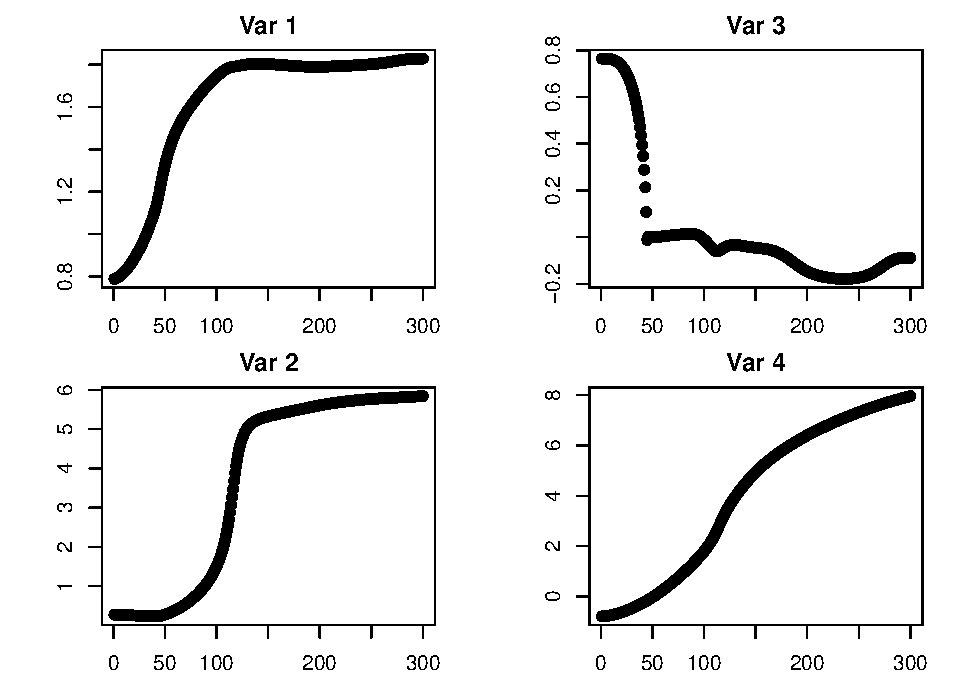
\includegraphics{_main_files/figure-latex/unnamed-chunk-6-1.pdf} 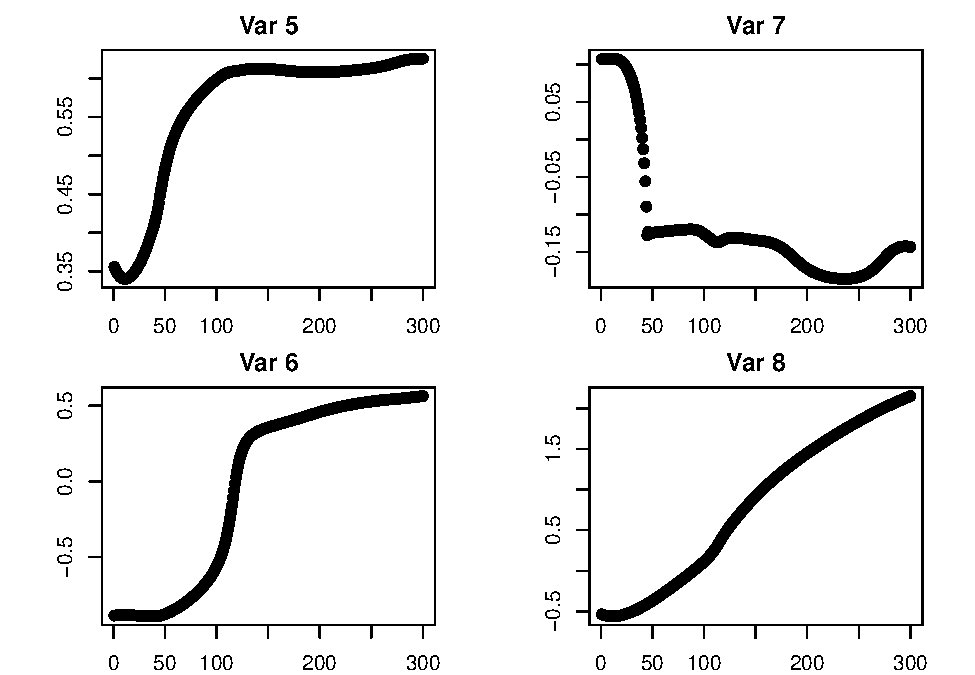
\includegraphics{_main_files/figure-latex/unnamed-chunk-6-2.pdf}

\begin{Shaded}
\begin{Highlighting}[]
\DocumentationTok{\#\# return to default}
\FunctionTok{par}\NormalTok{(}\AttributeTok{mfcol =} \FunctionTok{c}\NormalTok{(}\DecValTok{1}\NormalTok{, }\DecValTok{1}\NormalTok{))}
\end{Highlighting}
\end{Shaded}

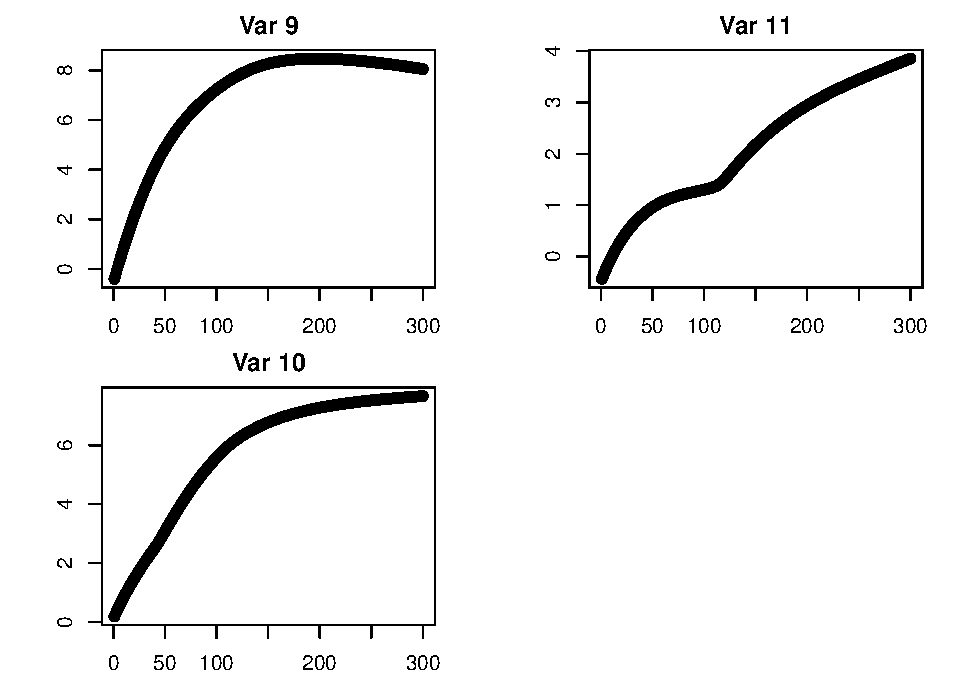
\includegraphics{_main_files/figure-latex/unnamed-chunk-6-3.pdf}

\begin{Shaded}
\begin{Highlighting}[]
\FunctionTok{par}\NormalTok{(}\AttributeTok{mar =} \FunctionTok{c}\NormalTok{(}\FloatTok{5.1}\NormalTok{, }\FloatTok{4.1}\NormalTok{, }\FloatTok{4.1}\NormalTok{, }\FloatTok{2.1}\NormalTok{))}
\end{Highlighting}
\end{Shaded}

\hypertarget{vectorized-calculations}{%
\section{Vectorized Calculations}\label{vectorized-calculations}}

A wayward attempt at deriving the matrix notation for vectorized operations that result in a simplified \(\nabla \mathcal{C}(\theta)\) by avoiding summations, to be replaced by strategic matrix multiplications.

This attempt was abandoned; there's more fertile ground in re-defining some notation and pursuing multi-layer networks (later chapters).

\hypertarget{notation-setup}{%
\subsection{Notation Setup}\label{notation-setup}}

We have our input matrix \(X\):

\[
X = 
\begin{bmatrix}
x_{1, 1} & x_{1, 2} & \cdots & x_{1, p} \\
x_{2, 1} & x_{2, 2} & \cdots & x_{2, p} \\
\vdots & \vdots & \ddots & \vdots \\
x_{n, 1} & x_{n, 2} & \cdots & x_{n, p} \\
\end{bmatrix}
\]

each row represents an obs (1-\emph{n})

each col represents a var (1-\emph{p})

\begin{center}\rule{0.5\linewidth}{0.5pt}\end{center}

our Weights matrix \(W\):

\[
W =
\begin{bmatrix}
w_{1, 1} & w_{2, 1} & \cdots & w_{K, 1} \\
w_{1, 2} & w_{2, 2} & \cdots & w_{K, 2} \\
\vdots & \vdots & \ddots & \vdots \\
w_{1, p} & w_{2, p} & \cdots & w_{K, p}
\end{bmatrix}
\]

each col represents a neuron (1-\emph{K})

each row represents a var (1-\emph{p})

\begin{center}\rule{0.5\linewidth}{0.5pt}\end{center}

our output layer weight matrix \(B\):

\[
B =
\begin{bmatrix}
\beta_{1} \\
\vdots \\
\beta_{K}
\end{bmatrix}
\]

each row represents a neuron (1-\emph{K})

\begin{center}\rule{0.5\linewidth}{0.5pt}\end{center}

our bias matrices \(b_1\), \(b_2\):

\[
b_1 =
\begin{bmatrix}
| & | &  & | \\
w_{1, 0} & w_{2, 0} & \cdots & w_{K, 0} \\
| & | &  & |
\end{bmatrix}
\]

\[
b_2 = \begin{bmatrix} | \\ \beta_0 \\ | \end{bmatrix}
\]

for \(b_1\), each col has a height of \(n\) and represents a neuron (1-\emph{K})

for \(b_2\), the col has a height of \(K\)

\begin{center}\rule{0.5\linewidth}{0.5pt}\end{center}

our target layer matrix \(Y\):

\[
Y =
\begin{bmatrix}
y_1 \\
y_2 \\
\vdots \\
y_n
\end{bmatrix}
\]

\begin{center}\rule{0.5\linewidth}{0.5pt}\end{center}

also, we have defined: \(z_{ik} = w_{k0} + \sum_{j = 1}^p w_{kj} x_{ij}\) to get the activation function's input for a given neuron. We can take the neurons in their totality to define \(Z\):

\[Z = X \cdot W + b_1\]

each row represents an obs (1-\emph{n})

each col represents a neuron (1-\emph{K})

\begin{center}\rule{0.5\linewidth}{0.5pt}\end{center}

our model output is \(\hat Y\):

\[
\begin{aligned}
\hat Y = f(X) &= g(Z) \cdot B + b_2 \\
&= g(X \cdot W + b_1) \cdot B + b_2 \\ \\
&= g\left(\begin{bmatrix}
x_{1, 1} & x_{1, 2} & \cdots & x_{1, p} \\
x_{2, 1} & x_{2, 2} & \cdots & x_{2, p} \\
\vdots & \vdots & \ddots & \vdots \\
x_{n, 1} & x_{n, 2} & \cdots & x_{n, p} \\
\end{bmatrix} \cdot \begin{bmatrix}
w_{1, 1} & w_{2, 1} & \cdots & w_{K, 1} \\
w_{1, 2} & w_{2, 2} & \cdots & w_{K, 2} \\
\vdots & \vdots & \ddots & \vdots \\
w_{1, p} & w_{2, p} & \cdots & w_{K, p}
\end{bmatrix} + \begin{bmatrix}
| & | &  & | \\
w_{1, 0} & w_{2, 0} & \cdots & w_{K, 0} \\
| & | &  & |
\end{bmatrix}\right) \cdot \begin{bmatrix}
\beta_{1} \\
\vdots \\
\beta_{K}
\end{bmatrix} + \begin{bmatrix} | \\ \beta_0 \\ | \end{bmatrix} \\ \\
&= \begin{bmatrix}
\hat y_1 \\
\hat y_2 \\
\vdots \\
\hat y_n
\end{bmatrix}
\end{aligned}
\]

\begin{center}\rule{0.5\linewidth}{0.5pt}\end{center}

our error matrix:

\[\mathbf{\hat \epsilon}= Y - \hat Y\]

\hypertarget{gradients}{%
\subsection{gradients}\label{gradients}}

We can now vectorize our gradient, \(\nabla \mathcal{C}(\theta)\):

\hypertarget{b_2}{%
\subsubsection{b\_2}\label{b_2}}

\[
\begin{aligned}
\nabla \mathcal{C}(b_2) &= \sum_{i = 1}^n \hat \epsilon_i\\
&= [\mathbf 1]^T \mathbf{\hat \epsilon}
\end{aligned}
\]

\hypertarget{b}{%
\subsubsection{B}\label{b}}

\[
\begin{aligned}
\nabla \mathcal{C}(B) &=  \sum_{i = 1}^n 
\begin{bmatrix}
\hat \epsilon_i\ g(z_{i1}) \\
\hat \epsilon_i\ g(z_{i2}) \\
\vdots \\
\hat \epsilon_i\ g(z_{ik})
\end{bmatrix} \\ \\
&= [g(Z)]^T \cdot \mathbf{\hat \epsilon}
\end{aligned}
\]

\hypertarget{b_1}{%
\subsubsection{b\_1}\label{b_1}}

\[
\begin{aligned}
\nabla \mathcal{C}(b_1) &= \sum_{i = 1}^n 
\begin{bmatrix}
\hat \epsilon_i\ \beta_1 \ g'(z_{i1})  \\
\hat \epsilon_i\ \beta_2 \ g'(z_{i2}) \\
\vdots \\
\hat \epsilon_i\ \beta_K \ g'(z_{iK})
\end{bmatrix} \\ \\
&= \left([g'(Z)]^T \cdot \mathbf{\hat \epsilon}\right) \odot B
\end{aligned}
\]

where \(\odot\) is the element-wise multiplication operator

\hypertarget{w}{%
\subsubsection{W}\label{w}}

\[
\begin{aligned}
\nabla \mathcal{C}(W) &= \sum_{i = 1}^n 
\begin{bmatrix}
\hat \epsilon_i\ \beta_1 \ g'(z_{i1}) \ x_{i1}  \\
\hat \epsilon_i\ \beta_2 \ g'(z_{i2}) \ x_{i2} \\
\vdots \\
\hat \epsilon_i\ \beta_K \ g'(z_{iK}) \ x_{ip}
\end{bmatrix} \\ \\
&= \ ???
\end{aligned}
\]

\hypertarget{digit-model}{%
\chapter{Digit Model}\label{digit-model}}

In preparation for neural networks, we take a brief chapter to run other models on MNIST hand-written data. First we will run a binomial GLM on each digit and keep the maximum outputted likelihood as the predicted digit, then we will run a multinomial GLM to assess the likelihood of every digit simultaneously.

This chapter can be safely skipped / ignored.

\hypertarget{binomial-model}{%
\section{Binomial Model}\label{binomial-model}}

\hypertarget{setup-1}{%
\subsection{Setup}\label{setup-1}}

\begin{Shaded}
\begin{Highlighting}[]
\CommentTok{\# Loads the MNIST dataset, saves as an .RData file if not in WD}
\ControlFlowTok{if}\NormalTok{ (}\SpecialCharTok{!}\NormalTok{(}\FunctionTok{file.exists}\NormalTok{(}\StringTok{"mnist\_data.RData"}\NormalTok{))) \{}
  
  \CommentTok{\# \#\# installs older python version}
  \CommentTok{\# reticulate::install\_python("3.10:latest")}
  \CommentTok{\# keras::install\_keras(python\_version = "3.10")}
  \CommentTok{\# \#\# re{-}loads keras}
  \CommentTok{\# library(keras)}
  
  \DocumentationTok{\#\# get MNIST data}
\NormalTok{  mnist }\OtherTok{\textless{}{-}} \FunctionTok{dataset\_mnist}\NormalTok{()}
  \DocumentationTok{\#\# save to WD as .RData}
  \FunctionTok{save}\NormalTok{(mnist, }\AttributeTok{file =} \StringTok{"mnist\_data.RData"}\NormalTok{)}
  
\NormalTok{\} }\ControlFlowTok{else}\NormalTok{ \{}
  \DocumentationTok{\#\# read{-}in MNIST data}
  \FunctionTok{load}\NormalTok{(}\AttributeTok{file =} \StringTok{"mnist\_data.RData"}\NormalTok{)}
\NormalTok{\}}

\CommentTok{\# Access the training and testing sets}
\NormalTok{x\_train }\OtherTok{\textless{}{-}}\NormalTok{ mnist}\SpecialCharTok{$}\NormalTok{train}\SpecialCharTok{$}\NormalTok{x}
\NormalTok{y\_train }\OtherTok{\textless{}{-}}\NormalTok{ mnist}\SpecialCharTok{$}\NormalTok{train}\SpecialCharTok{$}\NormalTok{y}
\NormalTok{x\_test }\OtherTok{\textless{}{-}}\NormalTok{ mnist}\SpecialCharTok{$}\NormalTok{test}\SpecialCharTok{$}\NormalTok{x}
\NormalTok{y\_test }\OtherTok{\textless{}{-}}\NormalTok{ mnist}\SpecialCharTok{$}\NormalTok{test}\SpecialCharTok{$}\NormalTok{y}

\FunctionTok{rm}\NormalTok{(mnist)}
\end{Highlighting}
\end{Shaded}

\begin{Shaded}
\begin{Highlighting}[]
\DocumentationTok{\#\# plot function, from OG data}
\NormalTok{plot\_mnist }\OtherTok{\textless{}{-}} \ControlFlowTok{function}\NormalTok{(plt) \{}
  \DocumentationTok{\#\# create image}
  \FunctionTok{image}\NormalTok{(}\AttributeTok{x =} \DecValTok{1}\SpecialCharTok{:}\DecValTok{28}\NormalTok{,}
        \AttributeTok{y =} \DecValTok{1}\SpecialCharTok{:}\DecValTok{28}\NormalTok{,}
        \DocumentationTok{\#\# image is oriented incorrectly, this fixes it}
        \AttributeTok{z =} \FunctionTok{t}\NormalTok{(}\FunctionTok{apply}\NormalTok{(plt, }\DecValTok{2}\NormalTok{, rev)),}
        \DocumentationTok{\#\# 255:0 puts black on white canvas,}
        \DocumentationTok{\#\# changing to 0:255 puts white on black canvas}
        \AttributeTok{col =} \FunctionTok{gray}\NormalTok{((}\DecValTok{255}\SpecialCharTok{:}\DecValTok{0}\NormalTok{)}\SpecialCharTok{/}\DecValTok{255}\NormalTok{),}
        \AttributeTok{axes =} \ConstantTok{FALSE}\NormalTok{)}
  
  \DocumentationTok{\#\# create plot border}
  \FunctionTok{rect}\NormalTok{(}\AttributeTok{xleft =} \FloatTok{0.5}\NormalTok{,}
       \AttributeTok{ybottom =} \FloatTok{0.5}\NormalTok{,}
       \AttributeTok{xright =} \DecValTok{28} \SpecialCharTok{+} \FloatTok{0.5}\NormalTok{,}
       \AttributeTok{ytop =} \DecValTok{28} \SpecialCharTok{+} \FloatTok{0.5}\NormalTok{,}
       \AttributeTok{border =} \StringTok{"black"}\NormalTok{,}
       \AttributeTok{lwd =} \DecValTok{1}\NormalTok{)}
\NormalTok{\}}
\end{Highlighting}
\end{Shaded}

\begin{Shaded}
\begin{Highlighting}[]
\DocumentationTok{\#\# train data}

\CommentTok{\# initialize matrix}
\NormalTok{x\_train\_2 }\OtherTok{\textless{}{-}} \FunctionTok{matrix}\NormalTok{(}\AttributeTok{nrow =} \FunctionTok{nrow}\NormalTok{(x\_train),}
                    \AttributeTok{ncol =} \DecValTok{28}\SpecialCharTok{*}\DecValTok{28}\NormalTok{)}

\DocumentationTok{\#\# likely a faster way to do this in the future}
\ControlFlowTok{for}\NormalTok{ (i }\ControlFlowTok{in} \DecValTok{1}\SpecialCharTok{:}\FunctionTok{nrow}\NormalTok{(x\_train)) \{}
  \DocumentationTok{\#\# get each layer\textquotesingle{}s matrix image, stretch to 28\^{}2 x 1}
\NormalTok{  x\_train\_2[i, ] }\OtherTok{\textless{}{-}} \FunctionTok{matrix}\NormalTok{(x\_train[i, , ], }\DecValTok{1}\NormalTok{, }\DecValTok{28}\SpecialCharTok{*}\DecValTok{28}\NormalTok{)}
\NormalTok{\}}

\NormalTok{x\_train\_2 }\OtherTok{\textless{}{-}}\NormalTok{ x\_train\_2 }\SpecialCharTok{\%\textgreater{}\%}
  \FunctionTok{as.data.frame}\NormalTok{()}

\DocumentationTok{\#\# test data}
\NormalTok{x\_test\_2 }\OtherTok{\textless{}{-}} \FunctionTok{matrix}\NormalTok{(}\AttributeTok{nrow =} \FunctionTok{nrow}\NormalTok{(x\_test),}
                   \AttributeTok{ncol =} \DecValTok{28}\SpecialCharTok{*}\DecValTok{28}\NormalTok{)}

\ControlFlowTok{for}\NormalTok{ (i }\ControlFlowTok{in} \DecValTok{1}\SpecialCharTok{:}\FunctionTok{nrow}\NormalTok{(x\_test)) \{}
\NormalTok{  x\_test\_2[i, ] }\OtherTok{\textless{}{-}} \FunctionTok{matrix}\NormalTok{(x\_test[i, , ], }\DecValTok{1}\NormalTok{, }\DecValTok{28}\SpecialCharTok{*}\DecValTok{28}\NormalTok{)}
\NormalTok{\}}

\NormalTok{x\_test\_2 }\OtherTok{\textless{}{-}}\NormalTok{ x\_test\_2 }\SpecialCharTok{\%\textgreater{}\%}
  \FunctionTok{as.data.frame}\NormalTok{()}


\DocumentationTok{\#\# re{-}scale data}
\NormalTok{x\_train\_2 }\OtherTok{\textless{}{-}}\NormalTok{ x\_train\_2 }\SpecialCharTok{/} \DecValTok{256}
\NormalTok{x\_test\_2 }\OtherTok{\textless{}{-}}\NormalTok{ x\_test\_2 }\SpecialCharTok{/} \DecValTok{256}

\DocumentationTok{\#\# response}
\CommentTok{\# x\_test\_2$y \textless{}{-} y\_test}
\CommentTok{\# x\_train\_2$y \textless{}{-} y\_train}
\end{Highlighting}
\end{Shaded}

\hypertarget{model}{%
\subsection{Model}\label{model}}

\begin{Shaded}
\begin{Highlighting}[]
\DocumentationTok{\#\# for speed}
\CommentTok{\# n \textless{}{-} nrow(x\_train\_2)}
\NormalTok{n }\OtherTok{\textless{}{-}} \DecValTok{100}
\NormalTok{indices }\OtherTok{\textless{}{-}} \FunctionTok{sample}\NormalTok{(}\AttributeTok{x =} \DecValTok{1}\SpecialCharTok{:}\FunctionTok{nrow}\NormalTok{(x\_train\_2),}
                  \AttributeTok{size =}\NormalTok{ n)}

\DocumentationTok{\#\# init data}
\NormalTok{x\_glm }\OtherTok{\textless{}{-}}\NormalTok{ x\_train\_2[indices, ]}
\NormalTok{y\_glm }\OtherTok{\textless{}{-}}\NormalTok{ y\_train[indices]}
\NormalTok{train\_pred }\OtherTok{\textless{}{-}} \FunctionTok{list}\NormalTok{()}

\DocumentationTok{\#\# drop cols with all 0s}
\NormalTok{x\_glm }\OtherTok{\textless{}{-}}\NormalTok{ x\_glm[, (}\FunctionTok{colSums}\NormalTok{(x\_glm) }\SpecialCharTok{\textgreater{}} \DecValTok{0}\NormalTok{)]}
\end{Highlighting}
\end{Shaded}

\begin{Shaded}
\begin{Highlighting}[]
\DocumentationTok{\#\# 10 model method}
\ControlFlowTok{for}\NormalTok{ (i }\ControlFlowTok{in} \DecValTok{0}\SpecialCharTok{:}\DecValTok{9}\NormalTok{) \{}
\FunctionTok{print}\NormalTok{(i)}
  
\NormalTok{y\_glm\_i }\OtherTok{=}\NormalTok{ (y\_glm }\SpecialCharTok{==}\NormalTok{ i)}

\NormalTok{init\_model }\OtherTok{\textless{}{-}} \FunctionTok{cv.glmnet}\NormalTok{(}\AttributeTok{x =}\NormalTok{ x\_glm }\SpecialCharTok{\%\textgreater{}\%}\NormalTok{ as.matrix,}
                        \AttributeTok{y =}\NormalTok{ y\_glm\_i,}
                        \AttributeTok{family =}\NormalTok{ binomial,}
                        \AttributeTok{alpha =} \DecValTok{1}\NormalTok{)}

\NormalTok{train\_pred[[i }\SpecialCharTok{+} \DecValTok{1}\NormalTok{]] }\OtherTok{\textless{}{-}} \FunctionTok{predict}\NormalTok{(init\_model,}
\NormalTok{                               x\_glm }\SpecialCharTok{\%\textgreater{}\%}\NormalTok{ as.matrix,}
                               \AttributeTok{s =}\NormalTok{ init\_model}\SpecialCharTok{$}\NormalTok{lambda.min,}
                               \AttributeTok{type =} \StringTok{"response"}\NormalTok{)}
\NormalTok{\}}
\end{Highlighting}
\end{Shaded}

\begin{verbatim}
## [1] 0
## [1] 1
## [1] 2
## [1] 3
## [1] 4
## [1] 5
## [1] 6
## [1] 7
## [1] 8
## [1] 9
\end{verbatim}

\begin{Shaded}
\begin{Highlighting}[]
\DocumentationTok{\#\# format results}
\NormalTok{predictions }\OtherTok{\textless{}{-}} \FunctionTok{data.frame}\NormalTok{(train\_pred)}
\FunctionTok{names}\NormalTok{(predictions) }\OtherTok{\textless{}{-}} \FunctionTok{c}\NormalTok{(}\StringTok{"zero"}\NormalTok{,}
                        \StringTok{"one"}\NormalTok{,}
                        \StringTok{"two"}\NormalTok{,}
                        \StringTok{"three"}\NormalTok{,}
                        \StringTok{"four"}\NormalTok{,}
                        \StringTok{"five"}\NormalTok{,}
                        \StringTok{"six"}\NormalTok{,}
                        \StringTok{"seven"}\NormalTok{,}
                        \StringTok{"eight"}\NormalTok{,}
                        \StringTok{"nine"}\NormalTok{)}

\CommentTok{\#write.csv(predictions, "pred.csv", row.names = FALSE)}

\DocumentationTok{\#\# convert to numeric}
\NormalTok{max\_col }\OtherTok{\textless{}{-}} \FunctionTok{apply}\NormalTok{(}\AttributeTok{X =}\NormalTok{ predictions,}
                 \AttributeTok{MARGIN =} \DecValTok{1}\NormalTok{,}
                 \AttributeTok{FUN =} \ControlFlowTok{function}\NormalTok{(x) }\FunctionTok{names}\NormalTok{(x)[}\FunctionTok{which.max}\NormalTok{(x)])}

\NormalTok{word\_to\_number }\OtherTok{\textless{}{-}} \FunctionTok{c}\NormalTok{(}\StringTok{"zero"} \OtherTok{=} \DecValTok{0}\NormalTok{,}
                    \StringTok{"one"} \OtherTok{=} \DecValTok{1}\NormalTok{,}
                    \StringTok{"two"} \OtherTok{=} \DecValTok{2}\NormalTok{,}
                    \StringTok{"three"} \OtherTok{=} \DecValTok{3}\NormalTok{,}
                    \StringTok{"four"} \OtherTok{=} \DecValTok{4}\NormalTok{,}
                    \StringTok{"five"} \OtherTok{=} \DecValTok{5}\NormalTok{,}
                    \StringTok{"six"} \OtherTok{=} \DecValTok{6}\NormalTok{,}
                    \StringTok{"seven"} \OtherTok{=} \DecValTok{7}\NormalTok{,}
                    \StringTok{"eight"} \OtherTok{=} \DecValTok{8}\NormalTok{,}
                    \StringTok{"nine"} \OtherTok{=} \DecValTok{9}\NormalTok{)}

\NormalTok{preds }\OtherTok{\textless{}{-}}\NormalTok{ word\_to\_number[max\_col] }\SpecialCharTok{\%\textgreater{}\%}\NormalTok{ as.numeric}

\DocumentationTok{\#\# confusion matrix}
\FunctionTok{table}\NormalTok{(y\_glm, preds)}
\end{Highlighting}
\end{Shaded}

\begin{verbatim}
##      preds
## y_glm  0  1  2  3  4  5  6  7  8  9
##     0 10  0  0  0  0  0  0  0  0  0
##     1  0 12  0  0  0  0  0  0  0  0
##     2  0  0  7  0  0  0  0  0  0  0
##     3  0  0  0  9  0  0  0  0  0  0
##     4  0  0  0  0 10  0  0  0  0  0
##     5  0  0  0  0  0 16  0  0  0  0
##     6  0  0  0  0  0  0 12  0  0  0
##     7  0  0  0  0  0  0  0 11  0  0
##     8  2  0  1  0  0  3  0  0  3  0
##     9  0  0  0  0  2  0  0  0  0  2
\end{verbatim}

\begin{Shaded}
\begin{Highlighting}[]
\DocumentationTok{\#\# misclassification rate}
\FunctionTok{mean}\NormalTok{(}\SpecialCharTok{!}\NormalTok{(y\_glm }\SpecialCharTok{==}\NormalTok{ preds))}
\end{Highlighting}
\end{Shaded}

\begin{verbatim}
## [1] 0.08
\end{verbatim}

\hypertarget{multinomial-model}{%
\section{Multinomial Model}\label{multinomial-model}}

\hypertarget{setup-2}{%
\subsection{Setup}\label{setup-2}}

\begin{Shaded}
\begin{Highlighting}[]
\CommentTok{\# Loads the MNIST dataset, saves as an .RData file if not in WD}
\ControlFlowTok{if}\NormalTok{ (}\SpecialCharTok{!}\NormalTok{(}\FunctionTok{file.exists}\NormalTok{(}\StringTok{"mnist\_data.RData"}\NormalTok{))) \{}
  
  \CommentTok{\# \#\# installs older python version}
  \CommentTok{\# reticulate::install\_python("3.10:latest")}
  \CommentTok{\# keras::install\_keras(python\_version = "3.10")}
  \CommentTok{\# \#\# re{-}loads keras}
  \CommentTok{\# library(keras)}
  
  \DocumentationTok{\#\# get MNIST data}
\NormalTok{  mnist }\OtherTok{\textless{}{-}} \FunctionTok{dataset\_mnist}\NormalTok{()}
  \DocumentationTok{\#\# save to WD as .RData}
  \FunctionTok{save}\NormalTok{(mnist, }\AttributeTok{file =} \StringTok{"mnist\_data.RData"}\NormalTok{)}
  
\NormalTok{\} }\ControlFlowTok{else}\NormalTok{ \{}
  \DocumentationTok{\#\# read{-}in MNIST data}
  \FunctionTok{load}\NormalTok{(}\AttributeTok{file =} \StringTok{"mnist\_data.RData"}\NormalTok{)}
\NormalTok{\}}

\CommentTok{\# Access the training and testing sets}
\NormalTok{x\_train }\OtherTok{\textless{}{-}}\NormalTok{ mnist}\SpecialCharTok{$}\NormalTok{train}\SpecialCharTok{$}\NormalTok{x}
\NormalTok{y\_train }\OtherTok{\textless{}{-}}\NormalTok{ mnist}\SpecialCharTok{$}\NormalTok{train}\SpecialCharTok{$}\NormalTok{y}
\NormalTok{x\_test }\OtherTok{\textless{}{-}}\NormalTok{ mnist}\SpecialCharTok{$}\NormalTok{test}\SpecialCharTok{$}\NormalTok{x}
\NormalTok{y\_test }\OtherTok{\textless{}{-}}\NormalTok{ mnist}\SpecialCharTok{$}\NormalTok{test}\SpecialCharTok{$}\NormalTok{y}

\FunctionTok{rm}\NormalTok{(mnist)}
\end{Highlighting}
\end{Shaded}

\begin{Shaded}
\begin{Highlighting}[]
\DocumentationTok{\#\# plot function}
\NormalTok{plot\_mnist\_array }\OtherTok{\textless{}{-}} \ControlFlowTok{function}\NormalTok{(plt, }\AttributeTok{main\_label =} \ConstantTok{NA}\NormalTok{, }\AttributeTok{color =} \ConstantTok{FALSE}\NormalTok{, }\AttributeTok{dim\_n =} \DecValTok{28}\NormalTok{) \{}
  
  \DocumentationTok{\#\# setup color}
  \ControlFlowTok{if}\NormalTok{ (color }\SpecialCharTok{==} \ConstantTok{TRUE}\NormalTok{) \{}
\NormalTok{      colfunc }\OtherTok{\textless{}{-}} \FunctionTok{colorRampPalette}\NormalTok{(}\FunctionTok{c}\NormalTok{(}\StringTok{"red"}\NormalTok{, }\StringTok{"white"}\NormalTok{, }\StringTok{"blue"}\NormalTok{))}
      
\NormalTok{      min\_abs }\OtherTok{\textless{}{-}} \SpecialCharTok{{-}}\FunctionTok{max}\NormalTok{(}\FunctionTok{abs}\NormalTok{(}\FunctionTok{range}\NormalTok{(plt)))}
\NormalTok{      max\_abs }\OtherTok{\textless{}{-}} \FunctionTok{max}\NormalTok{(}\FunctionTok{abs}\NormalTok{(}\FunctionTok{range}\NormalTok{(plt)))}
      
\NormalTok{      col }\OtherTok{\textless{}{-}} \FunctionTok{colfunc}\NormalTok{(}\DecValTok{256}\NormalTok{)}
\NormalTok{  \} }\ControlFlowTok{else}\NormalTok{ \{}
\NormalTok{    col }\OtherTok{\textless{}{-}} \FunctionTok{gray}\NormalTok{((}\DecValTok{255}\SpecialCharTok{:}\DecValTok{0}\NormalTok{)}\SpecialCharTok{/}\DecValTok{255}\NormalTok{)}
\NormalTok{    min\_abs }\OtherTok{\textless{}{-}} \DecValTok{0}
\NormalTok{    max\_abs }\OtherTok{\textless{}{-}} \DecValTok{255}
\NormalTok{    \}}
  
  \DocumentationTok{\#\# create image}
  \FunctionTok{image}\NormalTok{(}\AttributeTok{x =} \DecValTok{1}\SpecialCharTok{:}\NormalTok{dim\_n,}
        \AttributeTok{y =} \DecValTok{1}\SpecialCharTok{:}\NormalTok{dim\_n,}
        \DocumentationTok{\#\# image is oriented incorrectly, this fixes it}
        \AttributeTok{z =} \FunctionTok{t}\NormalTok{(}\FunctionTok{apply}\NormalTok{(plt, }\DecValTok{2}\NormalTok{, rev)),}
        \AttributeTok{col =}\NormalTok{ col,}
        \AttributeTok{zlim =} \FunctionTok{c}\NormalTok{(min\_abs, max\_abs),}
        \AttributeTok{axes =} \ConstantTok{FALSE}\NormalTok{,}
        \AttributeTok{xlab =} \ConstantTok{NA}\NormalTok{,}
        \AttributeTok{ylab =} \ConstantTok{NA}\NormalTok{)}
  
  \DocumentationTok{\#\# create plot border}
  \FunctionTok{rect}\NormalTok{(}\AttributeTok{xleft =} \FloatTok{0.5}\NormalTok{,}
       \AttributeTok{ybottom =} \FloatTok{0.5}\NormalTok{,}
       \AttributeTok{xright =} \DecValTok{28} \SpecialCharTok{+} \FloatTok{0.5}\NormalTok{,}
       \AttributeTok{ytop =} \DecValTok{28} \SpecialCharTok{+} \FloatTok{0.5}\NormalTok{,}
       \AttributeTok{border =} \StringTok{"black"}\NormalTok{,}
       \AttributeTok{lwd =} \DecValTok{1}\NormalTok{)}
  
  \DocumentationTok{\#\# display prediction result}
  \FunctionTok{text}\NormalTok{(}\AttributeTok{x =} \DecValTok{2}\NormalTok{,}
       \AttributeTok{y =}\NormalTok{ dim\_n }\SpecialCharTok{{-}} \DecValTok{3}\NormalTok{,}
       \AttributeTok{labels =} \FunctionTok{ifelse}\NormalTok{(}\FunctionTok{is.na}\NormalTok{(main\_label),}
                       \StringTok{""}\NormalTok{,}
\NormalTok{                       main\_label),}
       \AttributeTok{col =} \FunctionTok{ifelse}\NormalTok{(color }\SpecialCharTok{==} \ConstantTok{TRUE}\NormalTok{,}
                    \StringTok{"black"}\NormalTok{,}
                    \StringTok{"red"}\NormalTok{),}
       \AttributeTok{cex =} \FloatTok{1.5}\NormalTok{)}
\NormalTok{\}}
\end{Highlighting}
\end{Shaded}

\begin{Shaded}
\begin{Highlighting}[]
\DocumentationTok{\#\# train data}

\CommentTok{\# initialize matrix}
\NormalTok{x\_train\_2 }\OtherTok{\textless{}{-}} \FunctionTok{matrix}\NormalTok{(}\AttributeTok{nrow =} \FunctionTok{nrow}\NormalTok{(x\_train),}
                    \AttributeTok{ncol =} \DecValTok{28}\SpecialCharTok{*}\DecValTok{28}\NormalTok{)}

\DocumentationTok{\#\# likely a faster way to do this in the future}
\ControlFlowTok{for}\NormalTok{ (i }\ControlFlowTok{in} \DecValTok{1}\SpecialCharTok{:}\FunctionTok{nrow}\NormalTok{(x\_train)) \{}
  \DocumentationTok{\#\# get each layer\textquotesingle{}s matrix image, stretch to 28\^{}2 x 1}
\NormalTok{  x\_train\_2[i, ] }\OtherTok{\textless{}{-}} \FunctionTok{matrix}\NormalTok{(x\_train[i, , ], }\DecValTok{1}\NormalTok{, }\DecValTok{28}\SpecialCharTok{*}\DecValTok{28}\NormalTok{)}
\NormalTok{\}}

\NormalTok{x\_train\_2 }\OtherTok{\textless{}{-}}\NormalTok{ x\_train\_2 }\SpecialCharTok{\%\textgreater{}\%}
  \FunctionTok{as.data.frame}\NormalTok{()}

\DocumentationTok{\#\# test data}
\NormalTok{x\_test\_2 }\OtherTok{\textless{}{-}} \FunctionTok{matrix}\NormalTok{(}\AttributeTok{nrow =} \FunctionTok{nrow}\NormalTok{(x\_test),}
                   \AttributeTok{ncol =} \DecValTok{28}\SpecialCharTok{*}\DecValTok{28}\NormalTok{)}

\ControlFlowTok{for}\NormalTok{ (i }\ControlFlowTok{in} \DecValTok{1}\SpecialCharTok{:}\FunctionTok{nrow}\NormalTok{(x\_test)) \{}
\NormalTok{  x\_test\_2[i, ] }\OtherTok{\textless{}{-}} \FunctionTok{matrix}\NormalTok{(x\_test[i, , ], }\DecValTok{1}\NormalTok{, }\DecValTok{28}\SpecialCharTok{*}\DecValTok{28}\NormalTok{)}
\NormalTok{\}}

\NormalTok{x\_test\_2 }\OtherTok{\textless{}{-}}\NormalTok{ x\_test\_2 }\SpecialCharTok{\%\textgreater{}\%}
  \FunctionTok{as.data.frame}\NormalTok{()}


\DocumentationTok{\#\# re{-}scale data}
\NormalTok{x\_train\_2 }\OtherTok{\textless{}{-}}\NormalTok{ x\_train\_2 }\SpecialCharTok{/} \DecValTok{256}
\NormalTok{x\_test\_2 }\OtherTok{\textless{}{-}}\NormalTok{ x\_test\_2 }\SpecialCharTok{/} \DecValTok{256}

\DocumentationTok{\#\# response}
\CommentTok{\# x\_test\_2$y \textless{}{-} y\_test}
\CommentTok{\# x\_train\_2$y \textless{}{-} y\_train}
\end{Highlighting}
\end{Shaded}

\hypertarget{model-1}{%
\subsection{Model}\label{model-1}}

\hypertarget{train}{%
\subsubsection{train}\label{train}}

\begin{Shaded}
\begin{Highlighting}[]
\DocumentationTok{\#\# set training data size}
\CommentTok{\# n \textless{}{-} nrow(x\_train\_2)}
\NormalTok{n }\OtherTok{\textless{}{-}} \DecValTok{100}

\NormalTok{indices }\OtherTok{\textless{}{-}} \FunctionTok{sample}\NormalTok{(}\AttributeTok{x =} \DecValTok{1}\SpecialCharTok{:}\FunctionTok{nrow}\NormalTok{(x\_train\_2),}
                  \AttributeTok{size =}\NormalTok{ n)}

\DocumentationTok{\#\# init data}
\NormalTok{x\_multi }\OtherTok{\textless{}{-}}\NormalTok{ x\_train\_2[indices, ]}
\NormalTok{y\_multi }\OtherTok{\textless{}{-}}\NormalTok{ y\_train[indices]}

\DocumentationTok{\#\# drop cols with all 0s}
\CommentTok{\#x\_multi \textless{}{-} x\_multi[, (colSums(x\_multi) \textgreater{} 0)]}
\end{Highlighting}
\end{Shaded}

\begin{Shaded}
\begin{Highlighting}[]
\DocumentationTok{\#\# for the sake of the coefficients viz, setting alpha = 0}
\NormalTok{init\_model }\OtherTok{\textless{}{-}} \FunctionTok{cv.glmnet}\NormalTok{(}\AttributeTok{x =}\NormalTok{ x\_multi }\SpecialCharTok{\%\textgreater{}\%}\NormalTok{ as.matrix,}
                        \AttributeTok{y =}\NormalTok{ y\_multi }\SpecialCharTok{\%\textgreater{}\%}\NormalTok{ factor,}
                        \AttributeTok{family =} \StringTok{"multinomial"}\NormalTok{,}
                        \AttributeTok{alpha =} \DecValTok{0}\NormalTok{)}
\end{Highlighting}
\end{Shaded}

\begin{verbatim}
## Warning in lognet(xd, is.sparse, ix, jx, y, weights, offset, alpha, nobs, : one
## multinomial or binomial class has fewer than 8 observations; dangerous ground

## Warning in lognet(xd, is.sparse, ix, jx, y, weights, offset, alpha, nobs, : one
## multinomial or binomial class has fewer than 8 observations; dangerous ground

## Warning in lognet(xd, is.sparse, ix, jx, y, weights, offset, alpha, nobs, : one
## multinomial or binomial class has fewer than 8 observations; dangerous ground

## Warning in lognet(xd, is.sparse, ix, jx, y, weights, offset, alpha, nobs, : one
## multinomial or binomial class has fewer than 8 observations; dangerous ground

## Warning in lognet(xd, is.sparse, ix, jx, y, weights, offset, alpha, nobs, : one
## multinomial or binomial class has fewer than 8 observations; dangerous ground

## Warning in lognet(xd, is.sparse, ix, jx, y, weights, offset, alpha, nobs, : one
## multinomial or binomial class has fewer than 8 observations; dangerous ground

## Warning in lognet(xd, is.sparse, ix, jx, y, weights, offset, alpha, nobs, : one
## multinomial or binomial class has fewer than 8 observations; dangerous ground

## Warning in lognet(xd, is.sparse, ix, jx, y, weights, offset, alpha, nobs, : one
## multinomial or binomial class has fewer than 8 observations; dangerous ground

## Warning in lognet(xd, is.sparse, ix, jx, y, weights, offset, alpha, nobs, : one
## multinomial or binomial class has fewer than 8 observations; dangerous ground

## Warning in lognet(xd, is.sparse, ix, jx, y, weights, offset, alpha, nobs, : one
## multinomial or binomial class has fewer than 8 observations; dangerous ground

## Warning in lognet(xd, is.sparse, ix, jx, y, weights, offset, alpha, nobs, : one
## multinomial or binomial class has fewer than 8 observations; dangerous ground
\end{verbatim}

\begin{Shaded}
\begin{Highlighting}[]
\NormalTok{multi\_model }\OtherTok{\textless{}{-}} \FunctionTok{predict}\NormalTok{(init\_model,}
\NormalTok{                       x\_multi }\SpecialCharTok{\%\textgreater{}\%}\NormalTok{ as.matrix,}
                       \AttributeTok{s =}\NormalTok{ init\_model}\SpecialCharTok{$}\NormalTok{lambda.min,}
                       \AttributeTok{type =} \StringTok{"response"}\NormalTok{)}
\end{Highlighting}
\end{Shaded}

\begin{Shaded}
\begin{Highlighting}[]
\DocumentationTok{\#\# format results}
\NormalTok{preds\_init }\OtherTok{\textless{}{-}}\NormalTok{ multi\_model[, , }\DecValTok{1}\NormalTok{] }\SpecialCharTok{\%\textgreater{}\%}
  \FunctionTok{as.data.frame}\NormalTok{()}

\NormalTok{preds }\OtherTok{\textless{}{-}} \FunctionTok{apply}\NormalTok{(}\AttributeTok{X =}\NormalTok{ preds\_init,}
               \AttributeTok{MARGIN =} \DecValTok{1}\NormalTok{,}
               \AttributeTok{FUN =} \ControlFlowTok{function}\NormalTok{(x) }\FunctionTok{names}\NormalTok{(}\FunctionTok{which.max}\NormalTok{(x)) }\SpecialCharTok{\%\textgreater{}\%}\NormalTok{ as.numeric)}

\DocumentationTok{\#\# TRAIN confusion matrix}
\FunctionTok{table}\NormalTok{(y\_multi, preds)}
\end{Highlighting}
\end{Shaded}

\begin{verbatim}
##        preds
## y_multi  0  1  2  3  4  5  6  7  8  9
##       0 11  0  0  0  0  0  0  0  1  0
##       1  0 14  0  0  0  0  0  0  0  0
##       2  0  1  4  0  0  0  0  0  0  0
##       3  0  0  0 12  0  0  0  0  0  0
##       4  0  0  0  0 11  0  0  0  0  0
##       5  0  0  0  0  0  4  0  0  0  0
##       6  0  0  0  0  0  0 11  0  0  0
##       7  0  2  0  0  0  0  0  6  0  0
##       8  0  1  0  0  0  0  0  0 13  0
##       9  0  0  0  0  1  0  0  0  0  8
\end{verbatim}

\begin{Shaded}
\begin{Highlighting}[]
\DocumentationTok{\#\# TRAIN misclassification rate}
\FunctionTok{mean}\NormalTok{(}\SpecialCharTok{!}\NormalTok{(y\_multi }\SpecialCharTok{==}\NormalTok{ preds))}
\end{Highlighting}
\end{Shaded}

\begin{verbatim}
## [1] 0.06
\end{verbatim}

\hypertarget{test}{%
\subsubsection{test}\label{test}}

\begin{Shaded}
\begin{Highlighting}[]
\DocumentationTok{\#\# pre{-}process data}
\NormalTok{x\_multi\_test }\OtherTok{\textless{}{-}}\NormalTok{ x\_test\_2 }\SpecialCharTok{\%\textgreater{}\%}
  \FunctionTok{select}\NormalTok{(}\FunctionTok{all\_of}\NormalTok{(}\FunctionTok{names}\NormalTok{(x\_multi)))}

\DocumentationTok{\#\# get preds}
\NormalTok{multi\_model\_test }\OtherTok{\textless{}{-}} \FunctionTok{predict}\NormalTok{(init\_model,}
\NormalTok{                            x\_multi\_test }\SpecialCharTok{\%\textgreater{}\%}\NormalTok{ as.matrix,}
                            \AttributeTok{s =}\NormalTok{ init\_model}\SpecialCharTok{$}\NormalTok{lambda.min,}
                            \AttributeTok{type =} \StringTok{"response"}\NormalTok{)}
\end{Highlighting}
\end{Shaded}

\begin{Shaded}
\begin{Highlighting}[]
\DocumentationTok{\#\# format results}
\NormalTok{preds\_init\_test }\OtherTok{\textless{}{-}}\NormalTok{ multi\_model\_test[, , }\DecValTok{1}\NormalTok{] }\SpecialCharTok{\%\textgreater{}\%}
  \FunctionTok{as.data.frame}\NormalTok{()}

\NormalTok{preds\_test }\OtherTok{\textless{}{-}} \FunctionTok{apply}\NormalTok{(}\AttributeTok{X =}\NormalTok{ preds\_init\_test,}
               \AttributeTok{MARGIN =} \DecValTok{1}\NormalTok{,}
               \AttributeTok{FUN =} \ControlFlowTok{function}\NormalTok{(x) }\FunctionTok{names}\NormalTok{(}\FunctionTok{which.max}\NormalTok{(x)) }\SpecialCharTok{\%\textgreater{}\%}\NormalTok{ as.numeric)}

\DocumentationTok{\#\# }\AlertTok{TEST}\DocumentationTok{ confusion matrix}
\FunctionTok{table}\NormalTok{(y\_test, preds\_test)}
\end{Highlighting}
\end{Shaded}

\begin{verbatim}
##       preds_test
## y_test    0    1    2    3    4    5    6    7    8    9
##      0  859    1    2   10    7   16   26    1   55    3
##      1    0 1102    0    5    4    1    4    0   19    0
##      2   62  102  243  226   55   68   93   11  170    2
##      3   12   46   35  693    3    5    9   23  178    6
##      4    7   36    2    0  817   13   39    6   23   39
##      5   78   94    8  119   40  102   48   16  364   23
##      6   37   19    3   28   94    2  760    0   15    0
##      7    7   91    0    2   37    1    1  614   38  237
##      8   19   74    2   41    7   20   16    4  768   23
##      9   19   41    0    8  289    8    0  129  127  388
\end{verbatim}

\begin{Shaded}
\begin{Highlighting}[]
\DocumentationTok{\#\# }\AlertTok{TEST}\DocumentationTok{ misclassification rate}
\FunctionTok{mean}\NormalTok{(}\SpecialCharTok{!}\NormalTok{(y\_test }\SpecialCharTok{==}\NormalTok{ preds\_test))}
\end{Highlighting}
\end{Shaded}

\begin{verbatim}
## [1] 0.3654
\end{verbatim}

\begin{Shaded}
\begin{Highlighting}[]
\DocumentationTok{\#\# sort vectors so outputs are grouped}
\NormalTok{x\_test\_sort }\OtherTok{\textless{}{-}}\NormalTok{ x\_test[}\FunctionTok{order}\NormalTok{(y\_test), , ]}
\NormalTok{y\_test\_sort }\OtherTok{\textless{}{-}}\NormalTok{ y\_test[}\FunctionTok{order}\NormalTok{(y\_test)]}
\NormalTok{preds\_test\_sort }\OtherTok{\textless{}{-}}\NormalTok{ preds\_test[}\FunctionTok{order}\NormalTok{(y\_test)]}

\DocumentationTok{\#\# get misclassified obs}
\NormalTok{wrong }\OtherTok{\textless{}{-}} \FunctionTok{which}\NormalTok{(}\SpecialCharTok{!}\NormalTok{(y\_test\_sort }\SpecialCharTok{==}\NormalTok{ preds\_test\_sort))}

\DocumentationTok{\#\# plot a sample of misclassified obs}
\NormalTok{plot\_wrong }\OtherTok{\textless{}{-}}\NormalTok{ wrong[}\FunctionTok{sample}\NormalTok{(}\AttributeTok{x =} \DecValTok{1}\SpecialCharTok{:}\FunctionTok{length}\NormalTok{(wrong), }\AttributeTok{size =} \DecValTok{3}\SpecialCharTok{*}\DecValTok{8}\SpecialCharTok{*}\DecValTok{6}\NormalTok{)] }\SpecialCharTok{\%\textgreater{}\%}
  \FunctionTok{sort}\NormalTok{()}

\DocumentationTok{\#\# plot params}
\FunctionTok{par}\NormalTok{(}\AttributeTok{mfcol =} \FunctionTok{c}\NormalTok{(}\DecValTok{8}\NormalTok{, }\DecValTok{6}\NormalTok{))}
\FunctionTok{par}\NormalTok{(}\AttributeTok{mar =} \FunctionTok{c}\NormalTok{(}\DecValTok{0}\NormalTok{, }\DecValTok{0}\NormalTok{, }\DecValTok{0}\NormalTok{, }\DecValTok{0}\NormalTok{))}

\ControlFlowTok{for}\NormalTok{ (i }\ControlFlowTok{in}\NormalTok{ plot\_wrong) \{}
  \FunctionTok{plot\_mnist\_array}\NormalTok{(}\AttributeTok{plt =}\NormalTok{ x\_test\_sort[i, , ],}
                   \AttributeTok{main\_label =}\NormalTok{ preds\_test\_sort[i])}
\NormalTok{\}}
\end{Highlighting}
\end{Shaded}

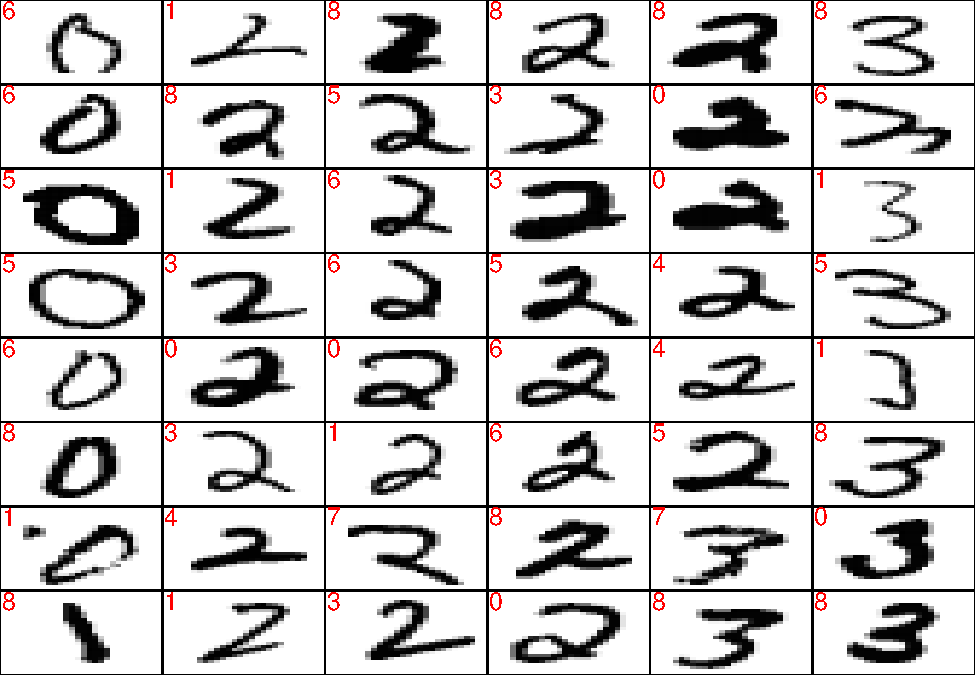
\includegraphics{_main_files/figure-latex/unnamed-chunk-21-1.pdf} 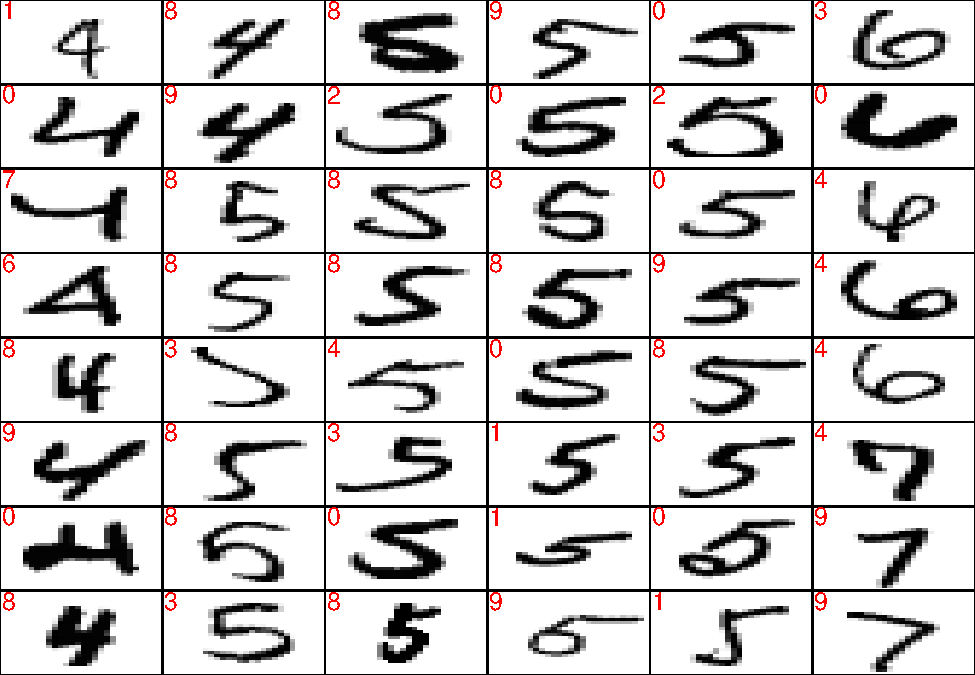
\includegraphics{_main_files/figure-latex/unnamed-chunk-21-2.pdf} 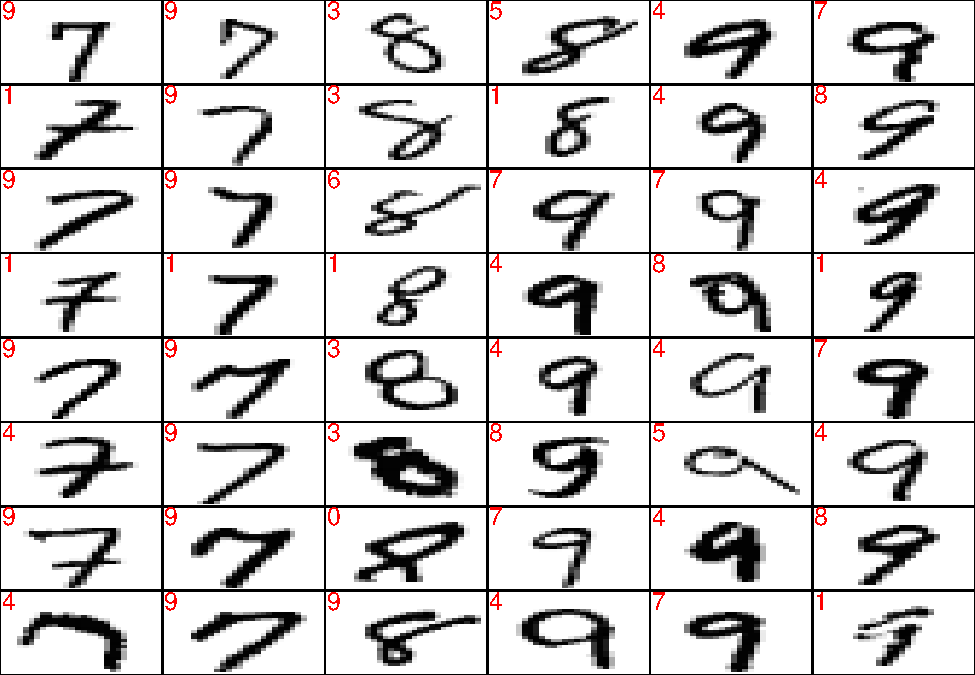
\includegraphics{_main_files/figure-latex/unnamed-chunk-21-3.pdf}

\begin{Shaded}
\begin{Highlighting}[]
\FunctionTok{par}\NormalTok{(}\AttributeTok{mfcol =} \FunctionTok{c}\NormalTok{(}\DecValTok{1}\NormalTok{, }\DecValTok{1}\NormalTok{))}
\end{Highlighting}
\end{Shaded}

\hypertarget{model-heatmaps}{%
\subsection{model heatmaps}\label{model-heatmaps}}

\begin{Shaded}
\begin{Highlighting}[]
\DocumentationTok{\#\# get coefficients into matrices}
\NormalTok{model\_coef }\OtherTok{\textless{}{-}} \FunctionTok{coef}\NormalTok{(init\_model, }\AttributeTok{s =}\NormalTok{ init\_model}\SpecialCharTok{$}\NormalTok{lambda.min) }\SpecialCharTok{\%\textgreater{}\%}
  \FunctionTok{lapply}\NormalTok{(as.matrix) }\SpecialCharTok{\%\textgreater{}\%}
  \FunctionTok{lapply}\NormalTok{(}\ControlFlowTok{function}\NormalTok{(x) }\FunctionTok{matrix}\NormalTok{(x[}\SpecialCharTok{{-}}\DecValTok{1}\NormalTok{, ], }\AttributeTok{nrow =} \DecValTok{28}\NormalTok{, }\AttributeTok{ncol =} \DecValTok{28}\NormalTok{)) }\SpecialCharTok{\%\textgreater{}\%}
  \DocumentationTok{\#\# take sigmoid activation just to help viz}
  \FunctionTok{lapply}\NormalTok{(}\ControlFlowTok{function}\NormalTok{(x) }\DecValTok{1} \SpecialCharTok{/}\NormalTok{ (}\DecValTok{1} \SpecialCharTok{+} \FunctionTok{exp}\NormalTok{(}\SpecialCharTok{{-}}\NormalTok{x)) }\SpecialCharTok{{-}} \FloatTok{0.5}\NormalTok{)}

\FunctionTok{mapply}\NormalTok{(}\AttributeTok{FUN =}\NormalTok{ plot\_mnist\_array,}
       \AttributeTok{plt =}\NormalTok{ model\_coef,}
       \AttributeTok{main\_label =} \FunctionTok{names}\NormalTok{(model\_coef),}
       \AttributeTok{color =} \ConstantTok{TRUE}\NormalTok{)}
\end{Highlighting}
\end{Shaded}

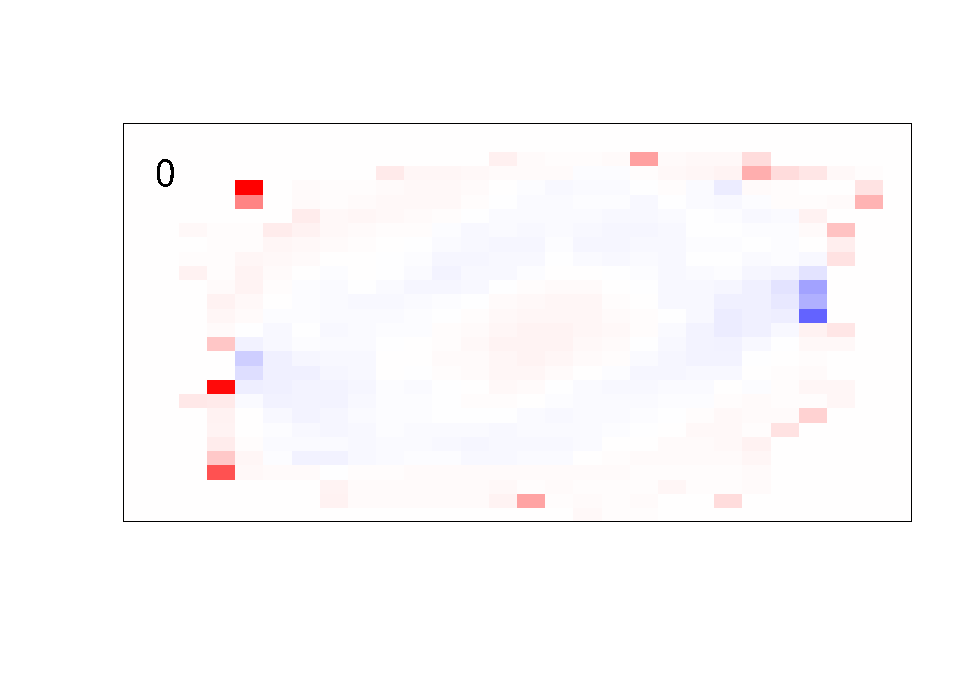
\includegraphics{_main_files/figure-latex/unnamed-chunk-22-1.pdf} 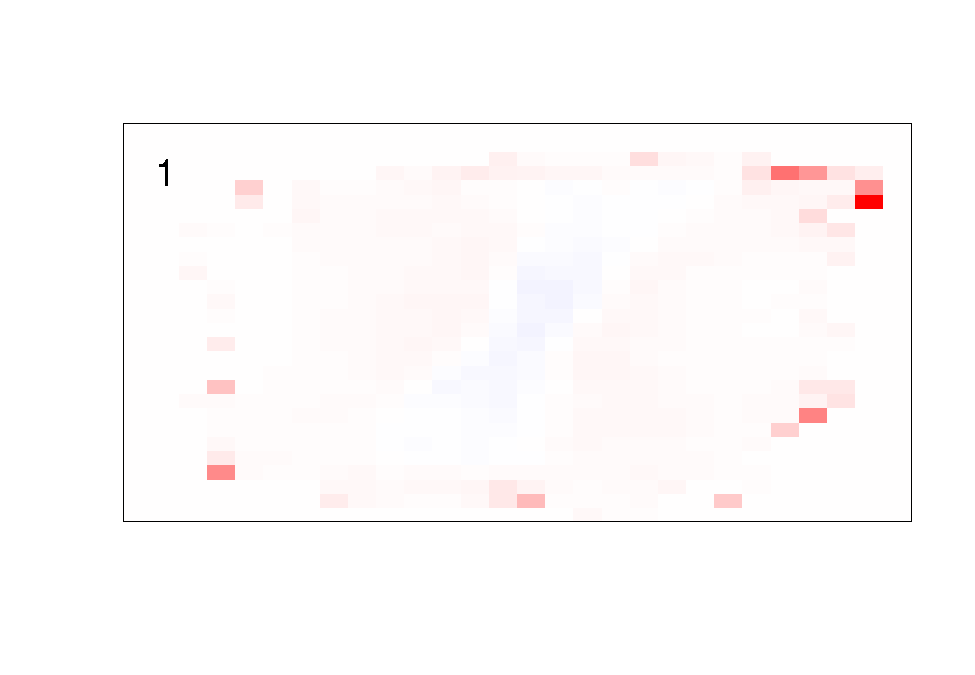
\includegraphics{_main_files/figure-latex/unnamed-chunk-22-2.pdf} 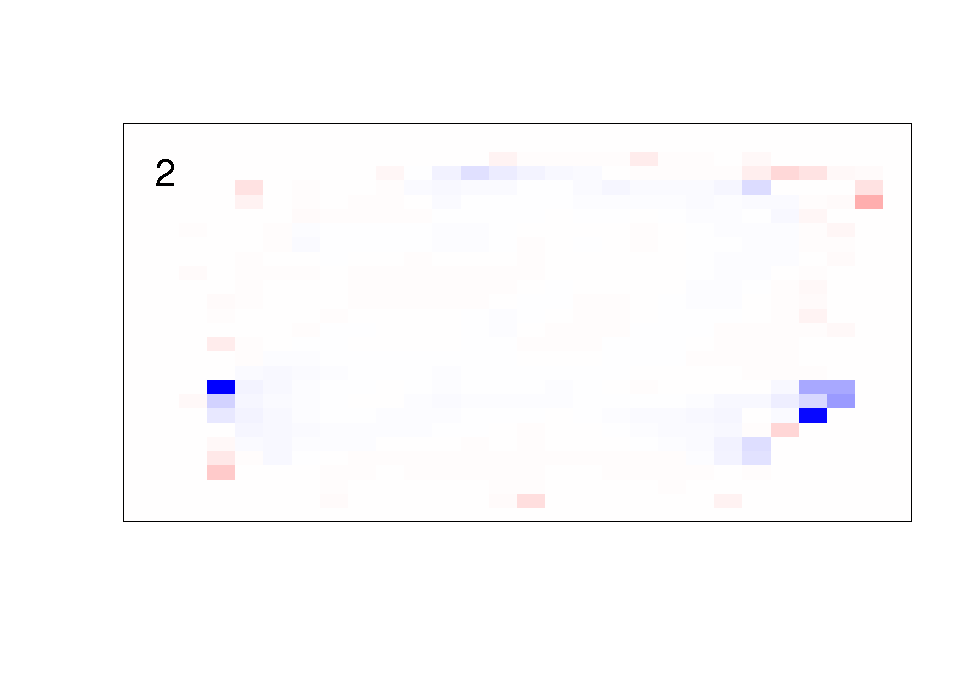
\includegraphics{_main_files/figure-latex/unnamed-chunk-22-3.pdf} 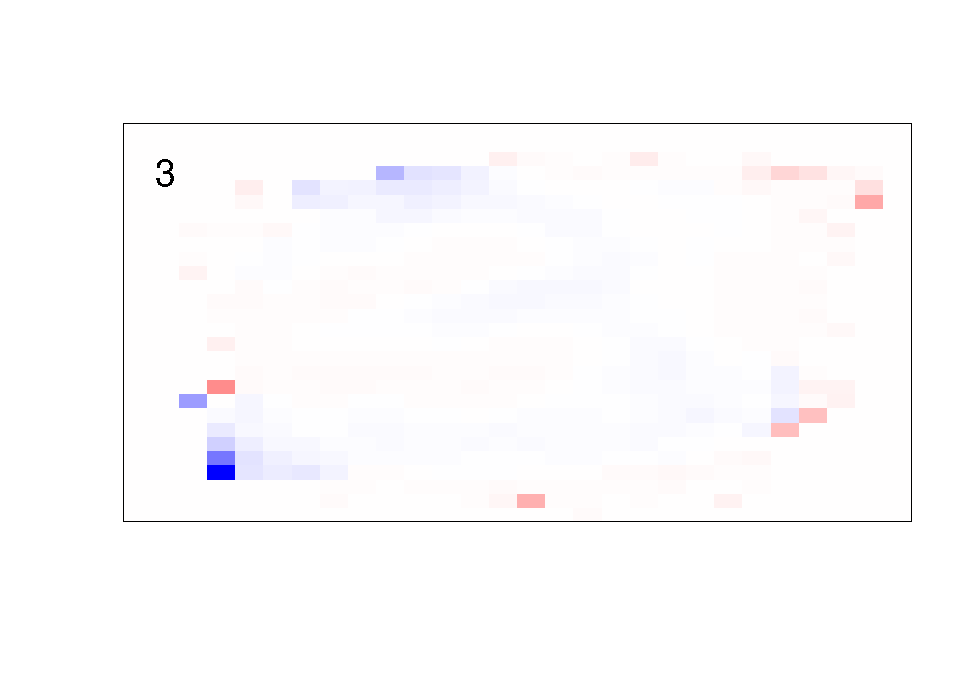
\includegraphics{_main_files/figure-latex/unnamed-chunk-22-4.pdf} 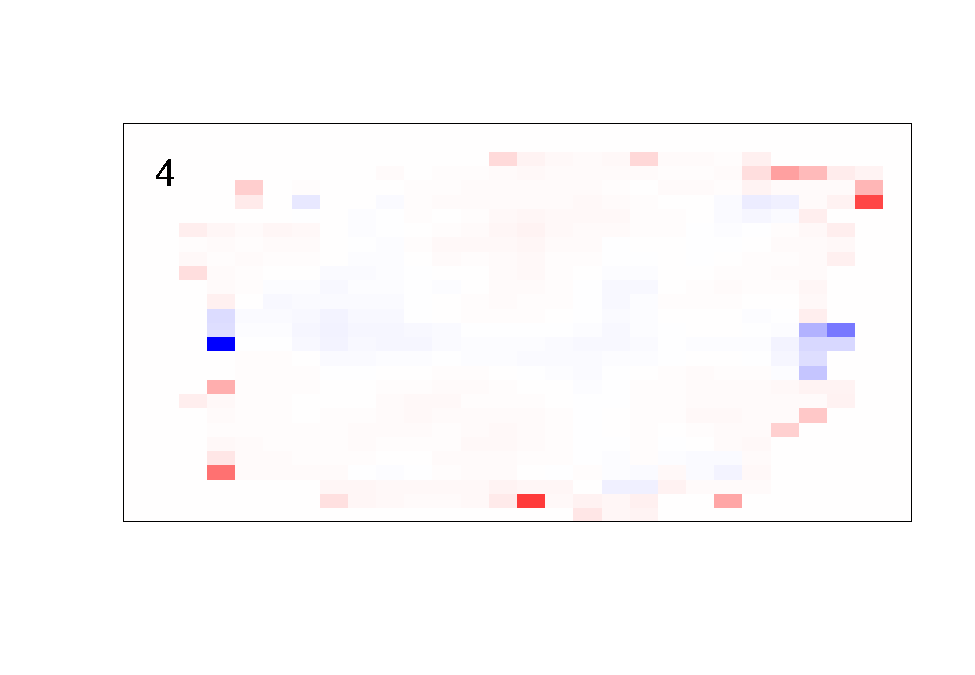
\includegraphics{_main_files/figure-latex/unnamed-chunk-22-5.pdf} 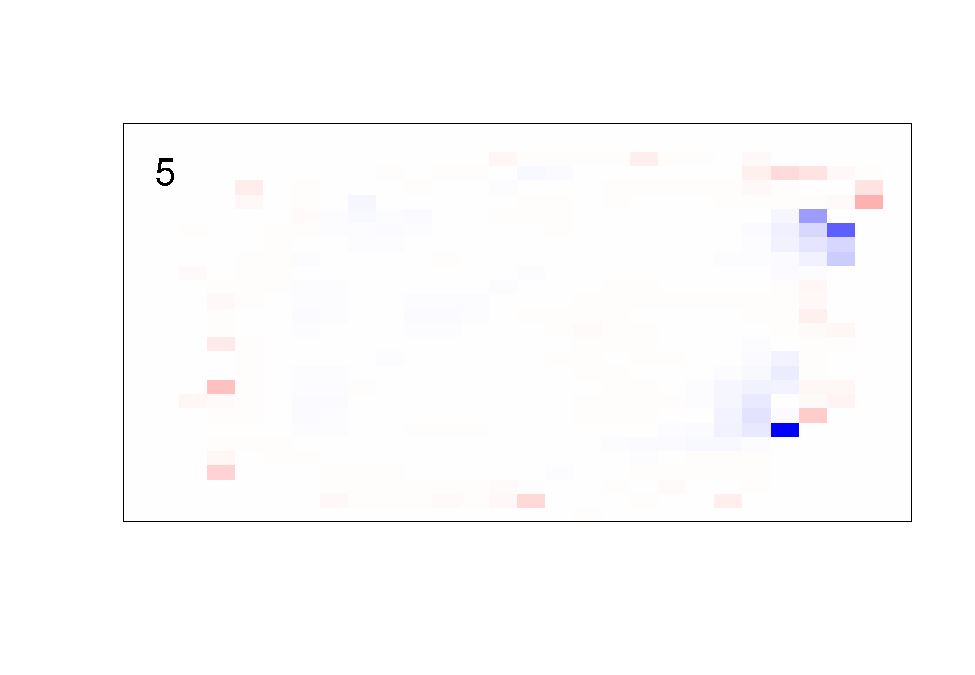
\includegraphics{_main_files/figure-latex/unnamed-chunk-22-6.pdf} 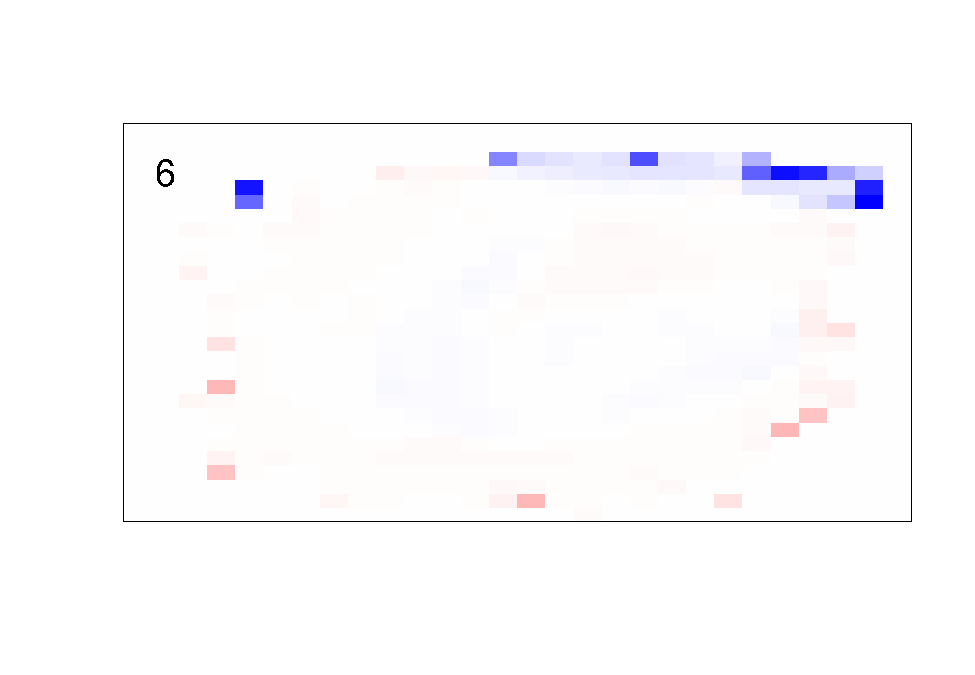
\includegraphics{_main_files/figure-latex/unnamed-chunk-22-7.pdf} 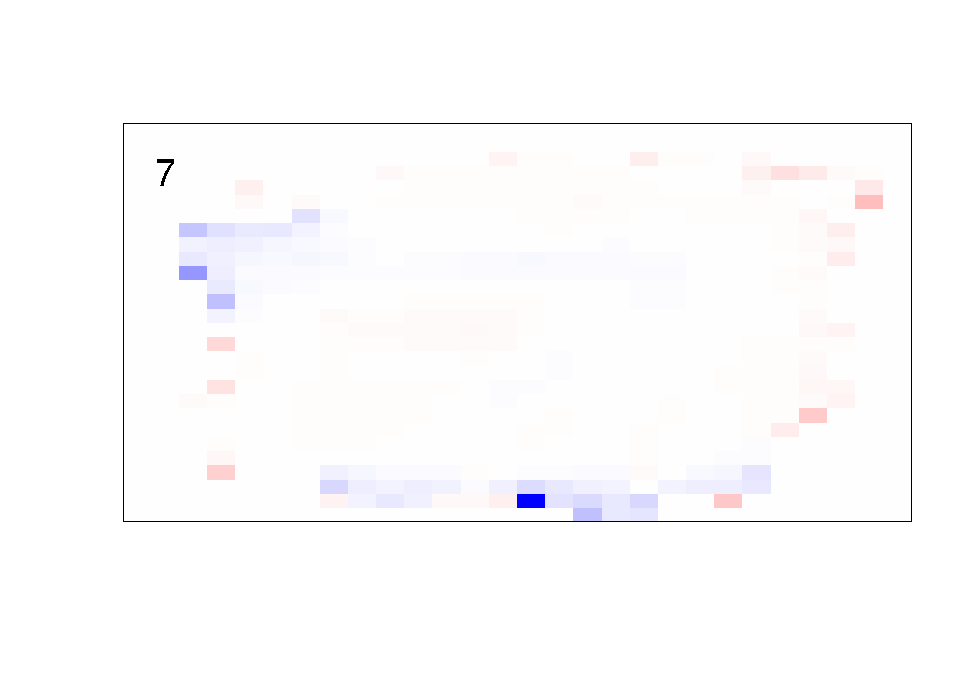
\includegraphics{_main_files/figure-latex/unnamed-chunk-22-8.pdf} 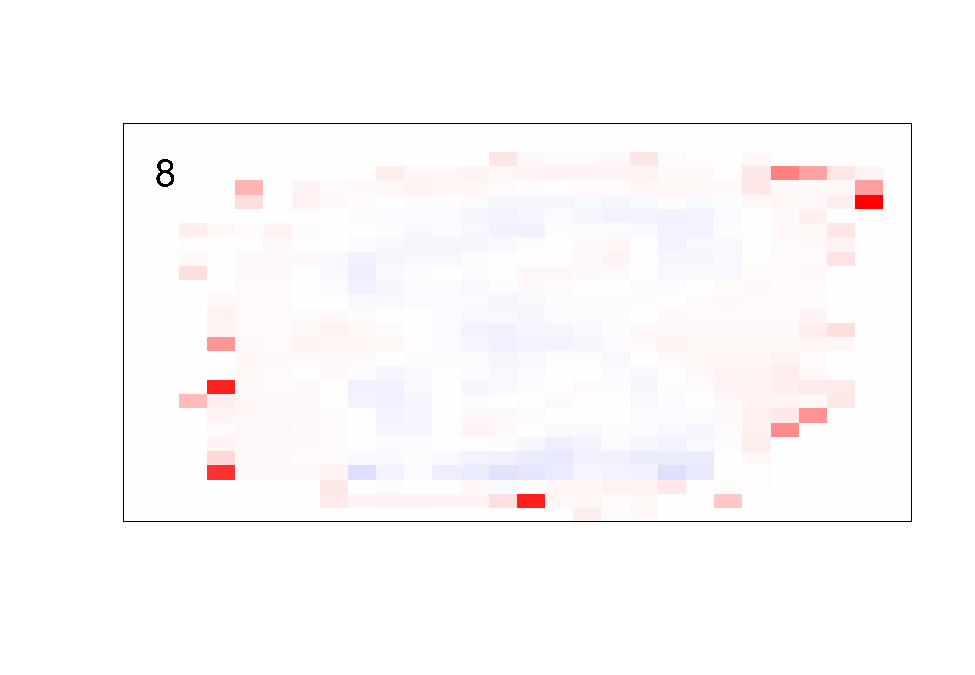
\includegraphics{_main_files/figure-latex/unnamed-chunk-22-9.pdf} 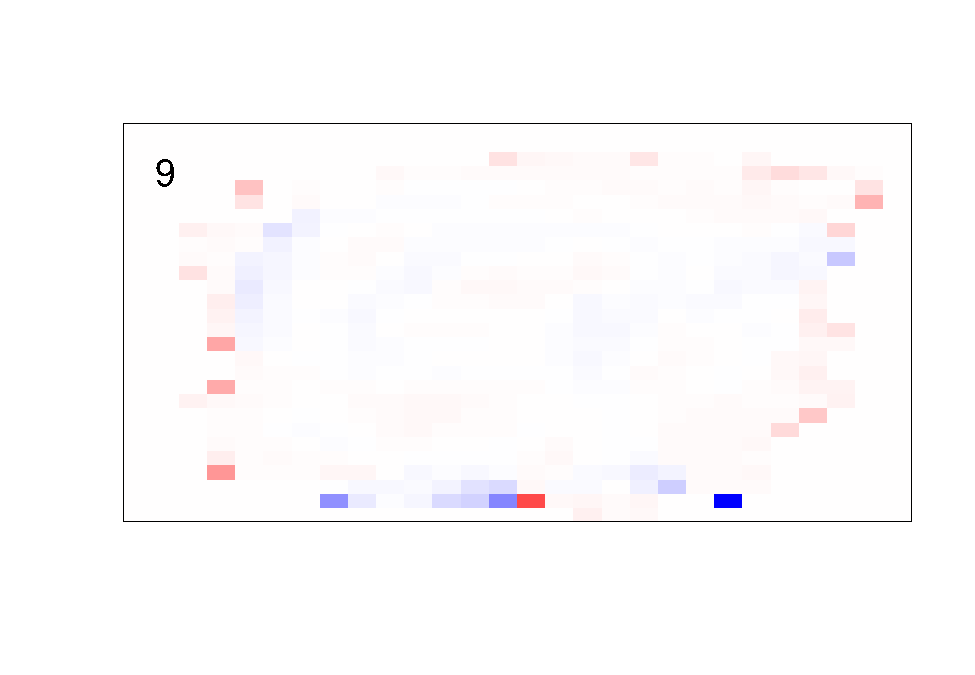
\includegraphics{_main_files/figure-latex/unnamed-chunk-22-10.pdf}

\begin{verbatim}
## $`0`
## NULL
## 
## $`1`
## NULL
## 
## $`2`
## NULL
## 
## $`3`
## NULL
## 
## $`4`
## NULL
## 
## $`5`
## NULL
## 
## $`6`
## NULL
## 
## $`7`
## NULL
## 
## $`8`
## NULL
## 
## $`9`
## NULL
\end{verbatim}

\hypertarget{no-outside-cells-model}{%
\subsection{no outside cells model}\label{no-outside-cells-model}}

earlier runs of the above sections revealed that for a regularization method that does not perform variable selection, odd importance is given to outermost cell for prediction. Thus, those will be removed:

\begin{Shaded}
\begin{Highlighting}[]
\DocumentationTok{\#\# set training data size}
\CommentTok{\# n \textless{}{-} nrow(x\_train\_2)}
\NormalTok{n }\OtherTok{\textless{}{-}} \DecValTok{100}

\NormalTok{indices }\OtherTok{\textless{}{-}} \FunctionTok{sample}\NormalTok{(}\AttributeTok{x =} \DecValTok{1}\SpecialCharTok{:}\FunctionTok{nrow}\NormalTok{(x\_train\_2),}
                  \AttributeTok{size =}\NormalTok{ n)}

\DocumentationTok{\#\# init data}
\NormalTok{x\_multi }\OtherTok{\textless{}{-}}\NormalTok{ x\_train\_2[indices, ]}
\NormalTok{y\_multi }\OtherTok{\textless{}{-}}\NormalTok{ y\_train[indices]}

\DocumentationTok{\#\# drop outer cells}
\NormalTok{x\_multi }\OtherTok{\textless{}{-}}\NormalTok{ x\_multi[, }\FunctionTok{rep}\NormalTok{(}\FunctionTok{seq}\NormalTok{(}\DecValTok{146}\NormalTok{, }\DecValTok{622}\NormalTok{, }\DecValTok{28}\NormalTok{), }\AttributeTok{each =} \DecValTok{18}\NormalTok{) }\SpecialCharTok{+} \FunctionTok{rep}\NormalTok{(}\DecValTok{0}\SpecialCharTok{:}\DecValTok{17}\NormalTok{, }\AttributeTok{times =} \DecValTok{18}\NormalTok{)]}
\end{Highlighting}
\end{Shaded}

\begin{Shaded}
\begin{Highlighting}[]
\DocumentationTok{\#\# for the sake of the coefficients viz, setting alpha = 0}
\NormalTok{init\_model }\OtherTok{\textless{}{-}} \FunctionTok{cv.glmnet}\NormalTok{(}\AttributeTok{x =}\NormalTok{ x\_multi }\SpecialCharTok{\%\textgreater{}\%}\NormalTok{ as.matrix,}
                        \AttributeTok{y =}\NormalTok{ y\_multi }\SpecialCharTok{\%\textgreater{}\%}\NormalTok{ factor,}
                        \AttributeTok{family =} \StringTok{"multinomial"}\NormalTok{,}
                        \AttributeTok{alpha =} \DecValTok{0}\NormalTok{)}
\end{Highlighting}
\end{Shaded}

\begin{verbatim}
## Warning in lognet(xd, is.sparse, ix, jx, y, weights, offset, alpha, nobs, : one
## multinomial or binomial class has fewer than 8 observations; dangerous ground

## Warning in lognet(xd, is.sparse, ix, jx, y, weights, offset, alpha, nobs, : one
## multinomial or binomial class has fewer than 8 observations; dangerous ground

## Warning in lognet(xd, is.sparse, ix, jx, y, weights, offset, alpha, nobs, : one
## multinomial or binomial class has fewer than 8 observations; dangerous ground

## Warning in lognet(xd, is.sparse, ix, jx, y, weights, offset, alpha, nobs, : one
## multinomial or binomial class has fewer than 8 observations; dangerous ground

## Warning in lognet(xd, is.sparse, ix, jx, y, weights, offset, alpha, nobs, : one
## multinomial or binomial class has fewer than 8 observations; dangerous ground

## Warning in lognet(xd, is.sparse, ix, jx, y, weights, offset, alpha, nobs, : one
## multinomial or binomial class has fewer than 8 observations; dangerous ground

## Warning in lognet(xd, is.sparse, ix, jx, y, weights, offset, alpha, nobs, : one
## multinomial or binomial class has fewer than 8 observations; dangerous ground

## Warning in lognet(xd, is.sparse, ix, jx, y, weights, offset, alpha, nobs, : one
## multinomial or binomial class has fewer than 8 observations; dangerous ground

## Warning in lognet(xd, is.sparse, ix, jx, y, weights, offset, alpha, nobs, : one
## multinomial or binomial class has fewer than 8 observations; dangerous ground

## Warning in lognet(xd, is.sparse, ix, jx, y, weights, offset, alpha, nobs, : one
## multinomial or binomial class has fewer than 8 observations; dangerous ground

## Warning in lognet(xd, is.sparse, ix, jx, y, weights, offset, alpha, nobs, : one
## multinomial or binomial class has fewer than 8 observations; dangerous ground
\end{verbatim}

\begin{Shaded}
\begin{Highlighting}[]
\NormalTok{multi\_model }\OtherTok{\textless{}{-}} \FunctionTok{predict}\NormalTok{(init\_model,}
\NormalTok{                       x\_multi }\SpecialCharTok{\%\textgreater{}\%}\NormalTok{ as.matrix,}
                       \AttributeTok{s =}\NormalTok{ init\_model}\SpecialCharTok{$}\NormalTok{lambda.min,}
                       \AttributeTok{type =} \StringTok{"response"}\NormalTok{)}
\end{Highlighting}
\end{Shaded}

\begin{Shaded}
\begin{Highlighting}[]
\DocumentationTok{\#\# get coefficients into matrices}
\NormalTok{model\_coef }\OtherTok{\textless{}{-}} \FunctionTok{coef}\NormalTok{(init\_model, }\AttributeTok{s =}\NormalTok{ init\_model}\SpecialCharTok{$}\NormalTok{lambda.min) }\SpecialCharTok{\%\textgreater{}\%}
  \FunctionTok{lapply}\NormalTok{(as.matrix) }\SpecialCharTok{\%\textgreater{}\%}
  \FunctionTok{lapply}\NormalTok{(}\ControlFlowTok{function}\NormalTok{(x) }\FunctionTok{matrix}\NormalTok{(x[}\SpecialCharTok{{-}}\DecValTok{1}\NormalTok{, ], }\AttributeTok{nrow =} \DecValTok{18}\NormalTok{, }\AttributeTok{ncol =} \DecValTok{18}\NormalTok{)) }\SpecialCharTok{\%\textgreater{}\%}
  \DocumentationTok{\#\# take sigmoid activation just to help viz}
  \FunctionTok{lapply}\NormalTok{(}\ControlFlowTok{function}\NormalTok{(x) }\DecValTok{1} \SpecialCharTok{/}\NormalTok{ (}\DecValTok{1} \SpecialCharTok{+} \FunctionTok{exp}\NormalTok{(}\SpecialCharTok{{-}}\NormalTok{x)) }\SpecialCharTok{{-}} \FloatTok{0.5}\NormalTok{)}

\FunctionTok{mapply}\NormalTok{(}\AttributeTok{FUN =}\NormalTok{ plot\_mnist\_array,}
       \AttributeTok{plt =}\NormalTok{ model\_coef,}
       \AttributeTok{main\_label =} \FunctionTok{names}\NormalTok{(model\_coef),}
       \AttributeTok{color =} \ConstantTok{TRUE}\NormalTok{,}
       \AttributeTok{dim\_n =} \DecValTok{18}\NormalTok{)}
\end{Highlighting}
\end{Shaded}

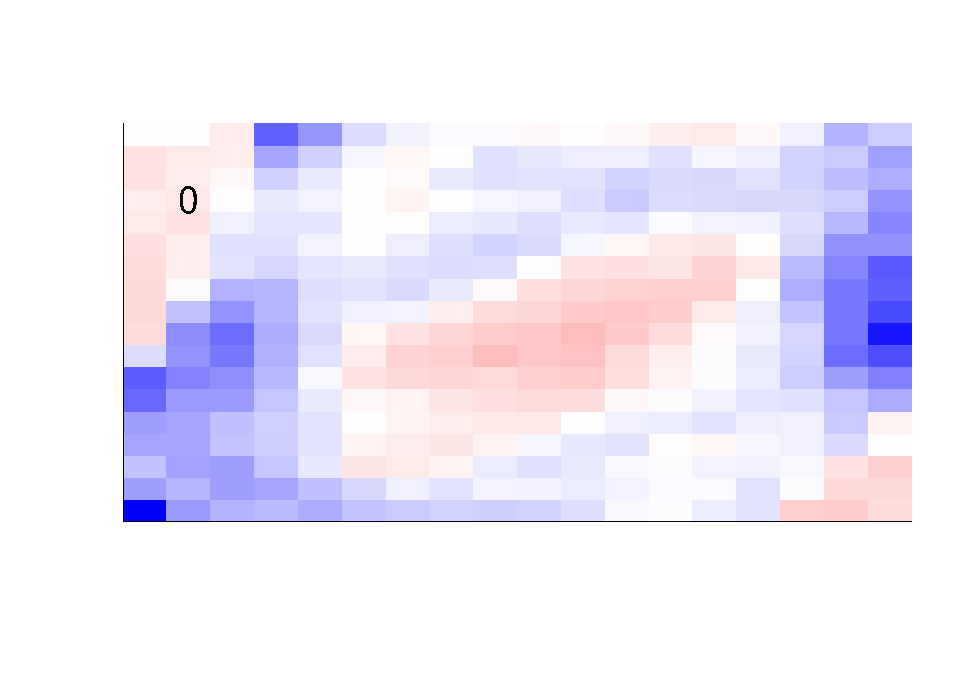
\includegraphics{_main_files/figure-latex/unnamed-chunk-25-1.pdf} 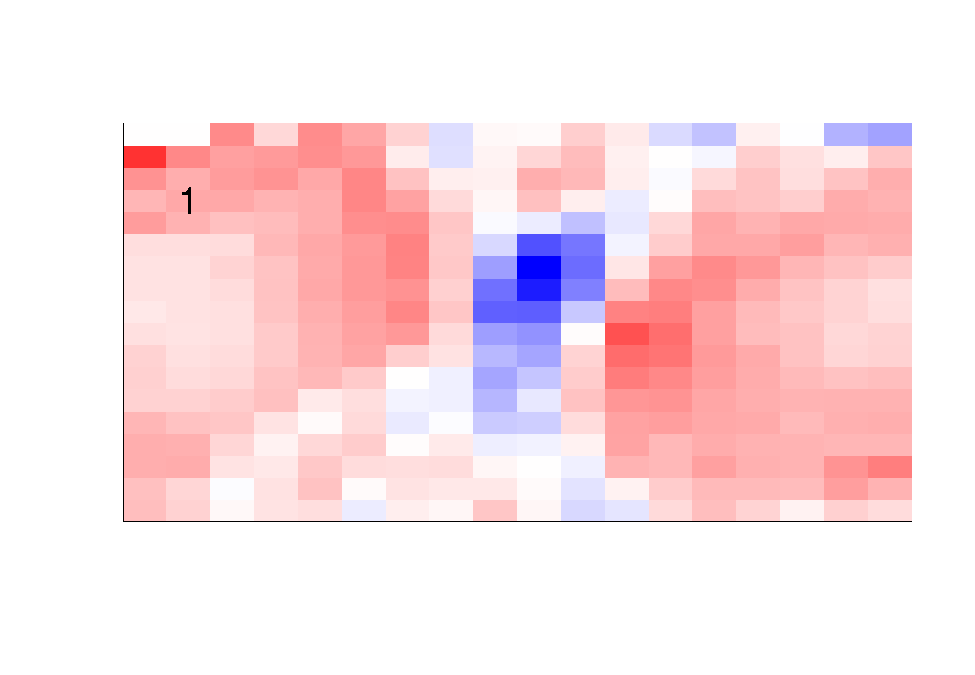
\includegraphics{_main_files/figure-latex/unnamed-chunk-25-2.pdf} 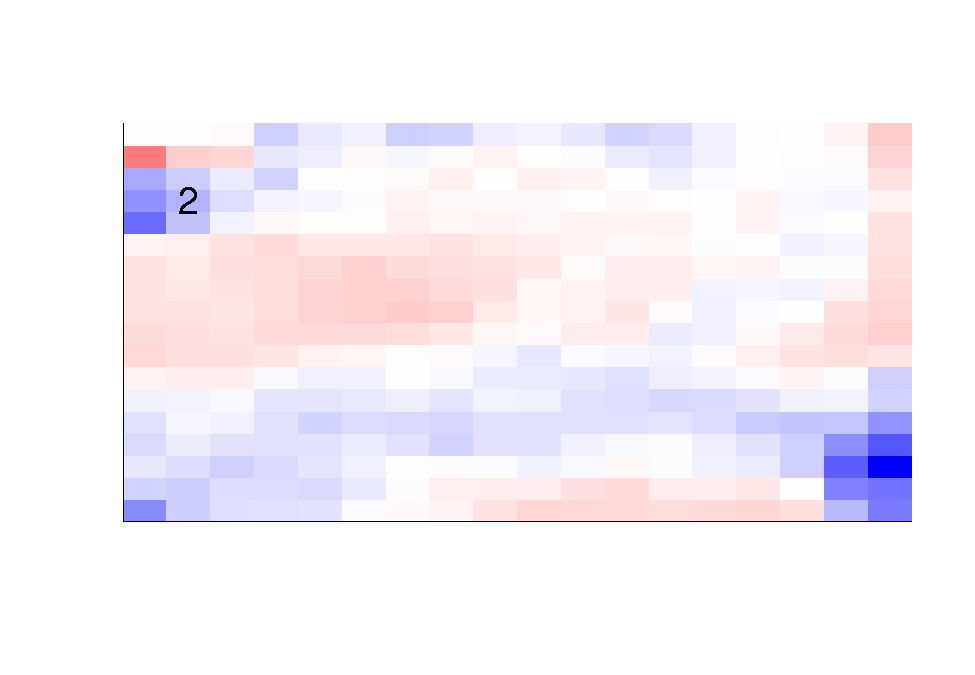
\includegraphics{_main_files/figure-latex/unnamed-chunk-25-3.pdf} 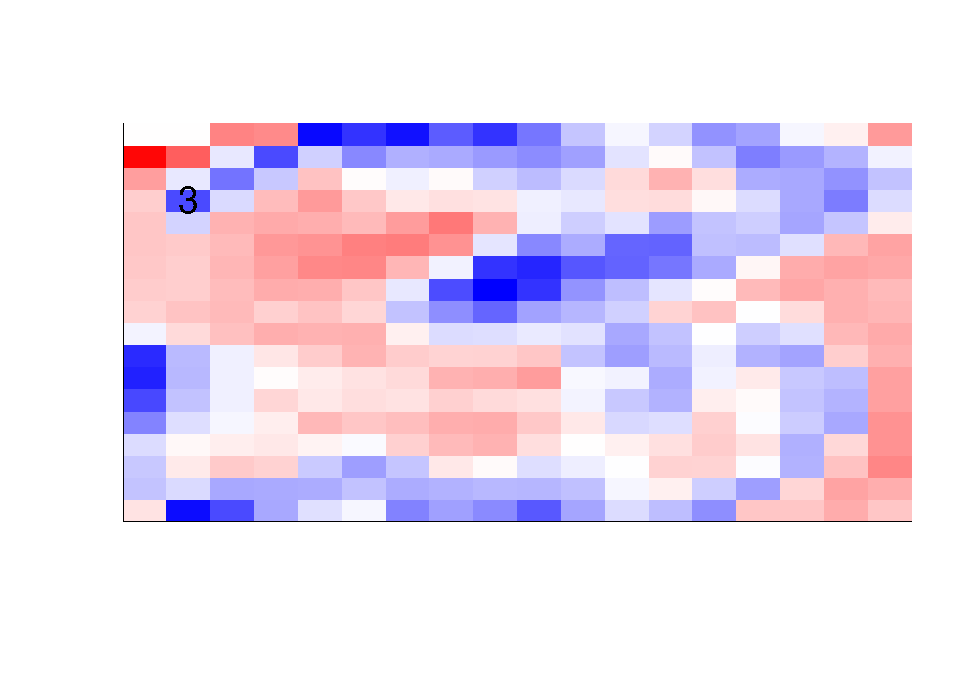
\includegraphics{_main_files/figure-latex/unnamed-chunk-25-4.pdf} 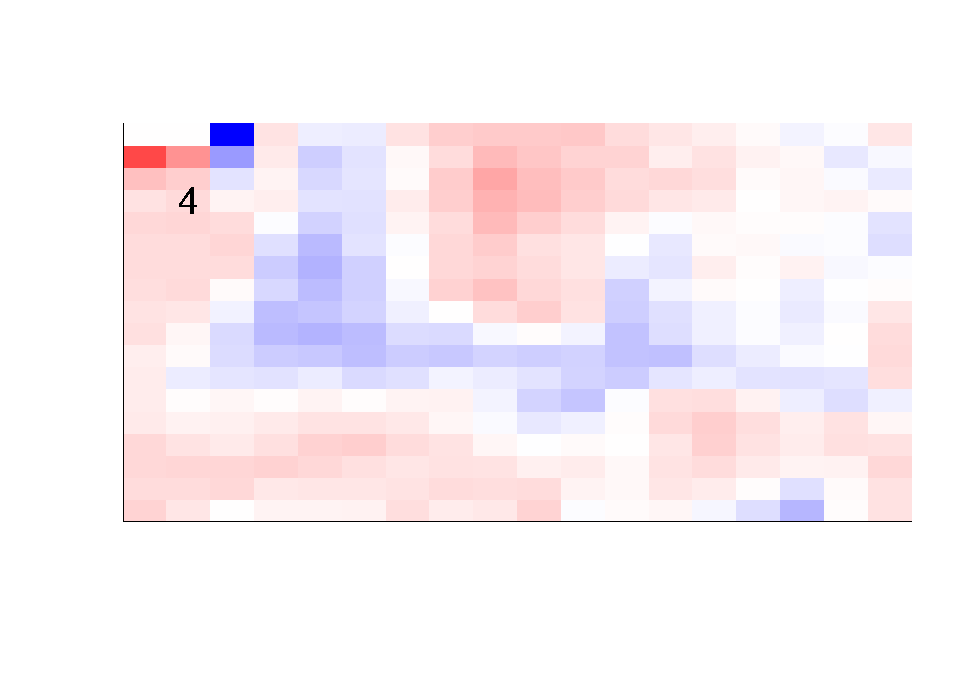
\includegraphics{_main_files/figure-latex/unnamed-chunk-25-5.pdf} 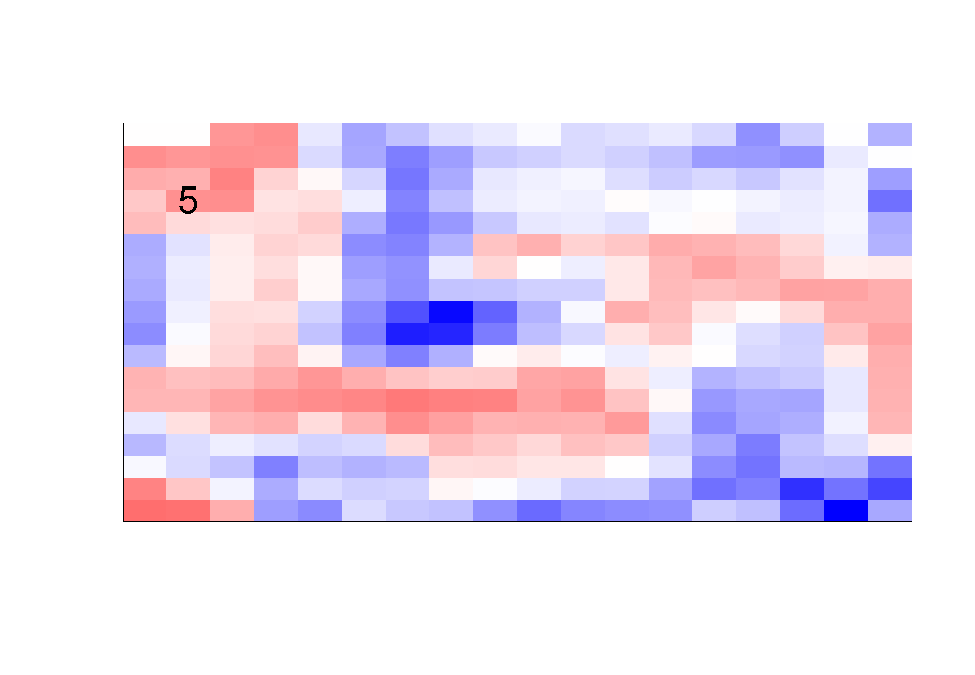
\includegraphics{_main_files/figure-latex/unnamed-chunk-25-6.pdf} 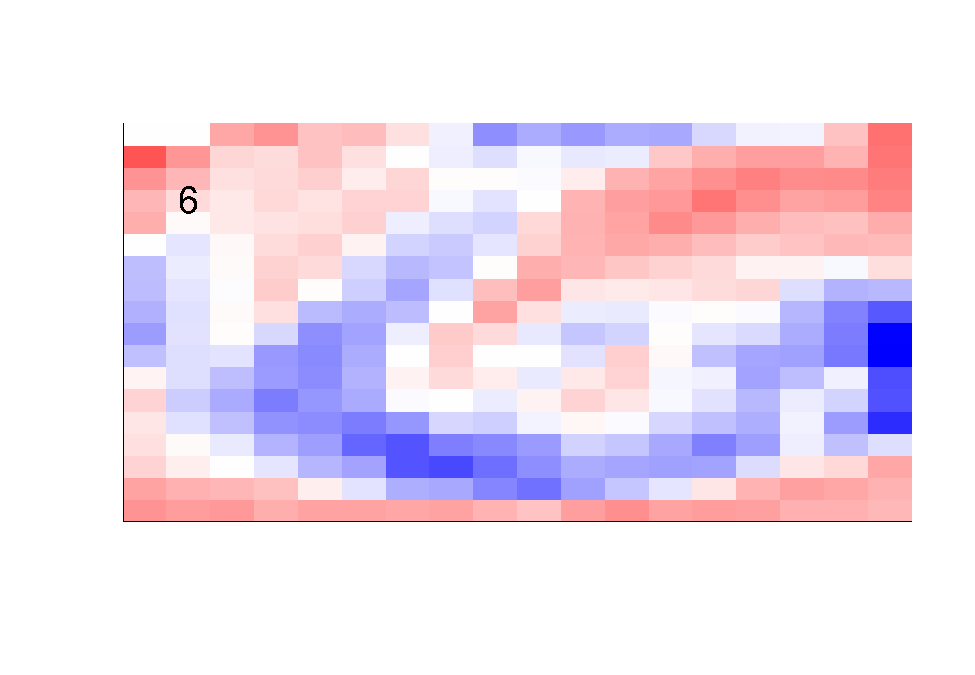
\includegraphics{_main_files/figure-latex/unnamed-chunk-25-7.pdf} 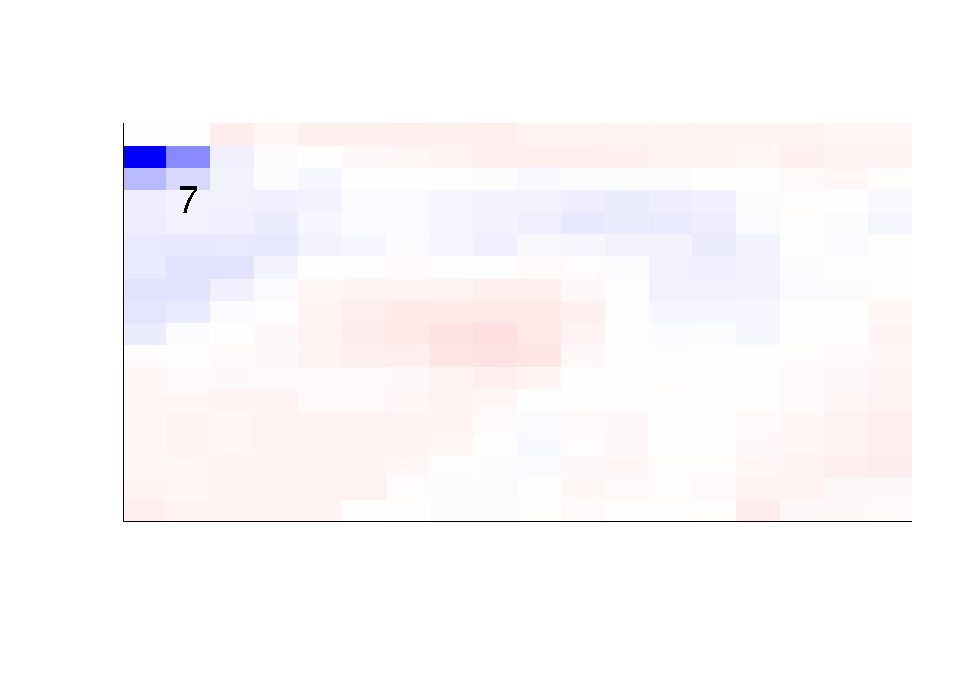
\includegraphics{_main_files/figure-latex/unnamed-chunk-25-8.pdf} 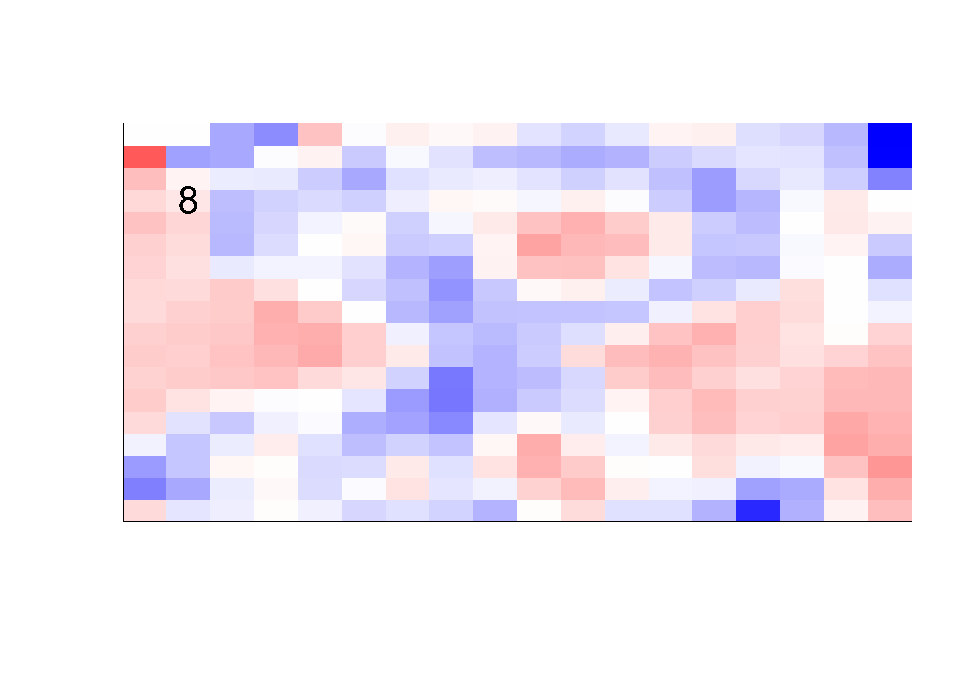
\includegraphics{_main_files/figure-latex/unnamed-chunk-25-9.pdf} 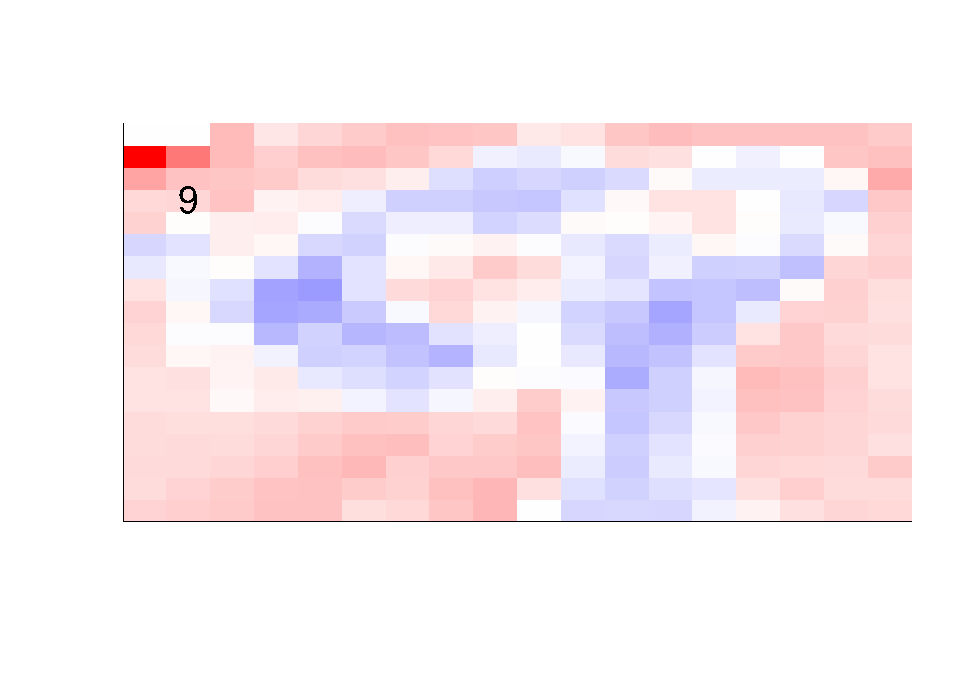
\includegraphics{_main_files/figure-latex/unnamed-chunk-25-10.pdf}

\begin{verbatim}
## $`0`
## NULL
## 
## $`1`
## NULL
## 
## $`2`
## NULL
## 
## $`3`
## NULL
## 
## $`4`
## NULL
## 
## $`5`
## NULL
## 
## $`6`
## NULL
## 
## $`7`
## NULL
## 
## $`8`
## NULL
## 
## $`9`
## NULL
\end{verbatim}

\hypertarget{multi-layer-nn-notes}{%
\chapter{Multi-Layer NN Notes}\label{multi-layer-nn-notes}}

Similar to the chapter on single-layer NNs, this chapter outlays notation \& methodology for a multiple-layer neural network.

\begin{center}\rule{0.5\linewidth}{0.5pt}\end{center}

source: \url{https://arxiv.org/abs/1801.05894}

``Deep Learning: An Introduction for Applied Mathematicians'' by Catherine F. Higham and Desmond J. Higham, published in 2018

\begin{center}\rule{0.5\linewidth}{0.5pt}\end{center}

\hypertarget{notation-setup-1}{%
\section{Notation Setup}\label{notation-setup-1}}

\hypertarget{scalars}{%
\subsection{Scalars}\label{scalars}}

Layers: 1-\(L\), indexed by \(l\)

Number of Neurons in layer \(l\): \(n_l\)

Neuron Activations: \(a^{(\text{layer num})}_{\text{neuron num}} = a^{(l)}_j\). Vector of activations for a layer is \(a^{(l)}\)

Activation Function: \(g(\cdot)\) is our generic activation function

\begin{center}\rule{0.5\linewidth}{0.5pt}\end{center}

\hypertarget{x}{%
\subsection{X}\label{x}}

We have our input matrix \(X \in \mathbb{R}^{\text{vars} \times \text{obs}} = \mathbb{R}^{n_0 \times m}\):

\[
X = \ ^{n_0 \text{ inputs}}
\overbrace{
  \begin{cases}
    \begin{bmatrix}
    x_{1, 1} & x_{1, 2} & \cdots & x_{1, m} \\
    x_{2, 1} & x_{2, 2} & \cdots & x_{2, m} \\
    \vdots & \vdots & \ddots & \vdots \\
    x_{n_0, 1} & x_{n_0, 2} & \cdots & x_{n_0, m} \\
    \end{bmatrix}
  \end{cases} 
}^{m \text{ obs}}
\]

The \(i\)th observation of \(X\) is the \(i\)th column of \(X\), referenced as \(x_i\).

\begin{center}\rule{0.5\linewidth}{0.5pt}\end{center}

\hypertarget{w-1}{%
\subsection{W}\label{w-1}}

our Weight matrices \(W^{(l)} \in \mathbb{R}^{\text{out} \times \text{in}} = \mathbb{R}^{n_l \times n_{l - 1}}\):

\[
W^{(l)} = \ ^{n_l\text{ outputs}}
\overbrace{
  \begin{cases}
    \begin{bmatrix}
    w^{(l)}_{1, 1} & w^{(l)}_{1, 2} & \cdots & w^{(l)}_{1, n_{l-1}} \\
    w^{(l)}_{2, 1} & w^{(l)}_{2, 2} & \cdots & w^{(l)}_{2, n_{l-1}} \\
    \vdots & \vdots & \ddots & \vdots \\
    w^{(l)}_{n_l, 1} & w^{(l)}_{n_l, 2} & \cdots & w^{(l)}_{n_l, n_{l-1}}
    \end{bmatrix}
  \end{cases} 
}^{n_{l - 1} \text{ inputs}}
\]

\(W^{(l)}\) is the weight matrix for the \(l\)th layer

\begin{center}\rule{0.5\linewidth}{0.5pt}\end{center}

\hypertarget{b-1}{%
\subsection{b}\label{b-1}}

our Bias matrices \(b^{(l)} \in \mathbb{R}^{\text{out} \times 1} = \mathbb{R}^{n_l \times 1}\):

\[
b^{(l)} = \ ^{n_l\text{ outputs}}
  \begin{cases}
    \begin{bmatrix}
    b^{(l)}_{1} \\
    b^{(l)}_{2} \\
    \vdots \\
    b^{(l)}_{n_l}
    \end{bmatrix}
  \end{cases}
\]

\(b^{(l)}\) is the bias matrix for the \(l\)th layer

\begin{center}\rule{0.5\linewidth}{0.5pt}\end{center}

\hypertarget{y}{%
\subsection{Y}\label{y}}

our target layer matrix \(Y \in \mathbb{R}^{\text{cats} \times \text{obs}} = \mathbb{R}^{n_L \times m}\):

\[
Y = \ ^{n_L \text{ categories}}
\overbrace{
  \begin{cases}
    \begin{bmatrix}
    y_{1, 1} & y_{1, 2} & \cdots & y_{1, m} \\
    y_{2, 1} & y_{2, 2} & \cdots & y_{2, m} \\
    \vdots & \vdots & \ddots & \vdots \\
    y_{n_L, 1} & y_{n_L, 2} & \cdots & y_{n_L, m}
    \end{bmatrix}
  \end{cases} 
}^{m \text{ obs}}
\]

Similar to \(X\), the \(i\)th observation of \(Y\) is the \(i\)th column of \(Y\), referenced as \(y_i\).

\begin{center}\rule{0.5\linewidth}{0.5pt}\end{center}

\hypertarget{z}{%
\subsection{z}\label{z}}

our neuron layer's activation function input \(z^{(l)} \in \mathbb{R}^{\text{out} \times 1} = \mathbb{R}^{n_l \times 1}\):

\[
z^{(l)} = \ ^{n_l\text{ outputs}}
  \begin{cases}
    \begin{bmatrix}
      z^{(l)}_{1} \\
      z^{(l)}_{2} \\
      \vdots \\
      z^{(l)}_{n_l}
    \end{bmatrix}
  \end{cases}
\]

\(z^{(l)}\) is the neuron `weighted input' matrix for the \(l\)th layer

We have that:

\[
\begin{aligned}
z^{(l)} &= W^{(l)} * a^{(l - 1)} + b^{(l)} \\ \\
&= \ ^{n_l\text{ outputs}}
\overbrace{
  \begin{cases}
    \begin{bmatrix}
    w^{(l)}_{1, 1} & w^{(l)}_{1, 2} & \cdots & w^{(l)}_{1, n_{l-1}} \\
    w^{(l)}_{2, 1} & w^{(l)}_{2, 2} & \cdots & w^{(l)}_{2, n_{l-1}} \\
    \vdots & \vdots & \ddots & \vdots \\
    w^{(l)}_{n_l, 1} & w^{(l)}_{n_l, 2} & \cdots & w^{(l)}_{n_l, n_{l-1}}
    \end{bmatrix}
  \end{cases} 
}^{n_{l - 1} \text{ inputs}} * \ ^{n_{l - 1} \text{ inputs}}
  \begin{cases}
    \begin{bmatrix}
      a^{(l-1)}_{1} \\
      a^{(l-1)}_{2} \\
      \vdots \\
      a^{(l-1)}_{n_l}
    \end{bmatrix}
  \end{cases} + \ ^{n_l\text{ outputs}}
  \begin{cases}
    \begin{bmatrix}
    b^{(l)}_{1} \\
    b^{(l)}_{2} \\
    \vdots \\
    b^{(l)}_{n_l}
    \end{bmatrix}
  \end{cases} \\ \\
&= \ ^{n_l\text{ outputs}}
  \begin{cases}
    \begin{bmatrix}
      z^{(l)}_{1} \\
      z^{(l)}_{2} \\
      \vdots \\
      z^{(l)}_{n_l}
    \end{bmatrix}
  \end{cases}
\end{aligned}
\]

\begin{center}\rule{0.5\linewidth}{0.5pt}\end{center}

\hypertarget{a}{%
\subsection{a}\label{a}}

our Neuron Activation \(a^{(l)} \in \mathbb{R}^{\text{out} \times 1} = \mathbb{R}^{n_l \times 1}\):

\[
a^{(l)} = \ ^{n_l\text{ outputs}}
  \begin{cases}
    \begin{bmatrix}
      a^{(l)}_{1} \\
      a^{(l)}_{2} \\
      \vdots \\
      a^{(l)}_{n_l}
    \end{bmatrix}
  \end{cases}
\]

\(a^{(l)}\) is the activation matrix for the \(l\)th layer

We have that:

\[
\begin{aligned}
a^{(l)} &= g\left(z^{(l)}\right) \\ \\
&= g\left(W^{(l)} * a^{(l - 1)} + b^{(l)}\right) \\ \\
&= g\left(\ ^{n_l\text{ outputs}}
\overbrace{
  \begin{cases}
    \begin{bmatrix}
    w^{(l)}_{1, 1} & w^{(l)}_{1, 2} & \cdots & w^{(l)}_{1, n_{l-1}} \\
    w^{(l)}_{2, 1} & w^{(l)}_{2, 2} & \cdots & w^{(l)}_{2, n_{l-1}} \\
    \vdots & \vdots & \ddots & \vdots \\
    w^{(l)}_{n_l, 1} & w^{(l)}_{n_l, 2} & \cdots & w^{(l)}_{n_l, n_{l-1}}
    \end{bmatrix}
  \end{cases} 
}^{n_{l - 1} \text{ inputs}} * \ ^{n_{l - 1} \text{ inputs}}
  \begin{cases}
    \begin{bmatrix}
      a^{(l-1)}_{1} \\
      a^{(l-1)}_{2} \\
      \vdots \\
      a^{(l-1)}_{n_l}
    \end{bmatrix}
  \end{cases} + \ ^{n_l\text{ outputs}}
  \begin{cases}
    \begin{bmatrix}
    b^{(l)}_{1} \\
    b^{(l)}_{2} \\
    \vdots \\
    b^{(l)}_{n_l}
    \end{bmatrix}
  \end{cases}\right) \\ \\
&= g\left(\ ^{n_l\text{ outputs}}
  \begin{cases}
    \begin{bmatrix}
      z^{(l)}_{1} \\
      z^{(l)}_{2} \\
      \vdots \\
      z^{(l)}_{n_l}
    \end{bmatrix}
  \end{cases}\right) \\ \\
&= \ ^{n_l\text{ outputs}}
  \begin{cases}
    \begin{bmatrix}
      a^{(l)}_{1} \\
      a^{(l)}_{2} \\
      \vdots \\
      a^{(l)}_{n_l}
    \end{bmatrix}
  \end{cases}
\end{aligned}
\]

\hypertarget{forward-propagation}{%
\section{Forward Propagation}\label{forward-propagation}}

\hypertarget{setup-3}{%
\subsection{Setup}\label{setup-3}}

For a single neuron, it's activation is going to be a weighted sum of all the activations of the previous layer, plus a constant, all fed into the activation function. Formally, this is:

\[a^{(l)}_j = g\left(\sum_{i = 1}^{n_{l - 1}} w^{(l)}_{j, i} * a^{(l - 1)}_{i} + b^{(l)}_{j}\right)\]

We can put this in matrix form. An entire layer of neurons can be represented by:

\[a^{(l)} = g\left(z^{(l)}\right) = g\left(W^{(l)} * a^{(l - 1)} + b^{(l)}\right)\]

as was shown above. We can repeatedly apply this formula to get from \(X\) to out predicted \(\hat Y = a^{(L)}\). We start with the initial layer (layer 0) being set equal to \(x_i\).

Note that we will be forward (\& backward) propagating one observation of \(X\) at a time by operating on each column separately. However, if desired forward (\& backward) propagation can be done on all observations simultaneously. The notation change would involve stretching out \(a^{(l)}\), \(z^{(l)}\), and \(b^{(l)}\) so that they are each \(m\) wide:

\[
\begin{aligned}
a^{(l)} &= g\left(z^{(l)}\right) \\ \\
&= g\left(W^{(l)} * a^{(l - 1)} + b^{(l)}\right) \\ \\
&= g(\ ^{n_l\text{ outputs}}
\overbrace{
  \begin{cases}
    \begin{bmatrix}
    w^{(l)}_{1, 1} & w^{(l)}_{1, 2} & \cdots & w^{(l)}_{1, n_{l-1}} \\
    w^{(l)}_{2, 1} & w^{(l)}_{2, 2} & \cdots & w^{(l)}_{2, n_{l-1}} \\
    \vdots & \vdots & \ddots & \vdots \\
    w^{(l)}_{n_l, 1} & w^{(l)}_{n_l, 2} & \cdots & w^{(l)}_{n_l, n_{l-1}}
    \end{bmatrix}
  \end{cases} 
}^{n_{l - 1} \text{ inputs}} * \ ^{n_{l - 1} \text{ inputs}}
\overbrace{
  \begin{cases}
    \begin{bmatrix}
    a^{(l - 1)}_{1, 1} & a^{(l - 1)}_{1, 2} & \cdots & a^{(l - 1)}_{1, m} \\
    a^{(l - 1)}_{2, 1} & a^{(l - 1)}_{2, 2} & \cdots & a^{(l - 1)}_{2, m} \\
    \vdots & \vdots & \ddots & \vdots \\
    a^{(l - 1)}_{n_{l - 1}, 1} & a^{(l - 1)}_{n_{l - 1}, 2} & \cdots & a^{(l - 1)}_{n_{l - 1}, m} \\
    \end{bmatrix}
  \end{cases} 
}^{m \text{ obs}} \\
&+ \ ^{n_l \text{ outputs}}
\overbrace{
  \begin{cases}
    \begin{bmatrix}
    - & b^{(l)}_{1} & - \\
    - & b^{(l)}_{2} & - \\
    \vdots & \vdots & \vdots \\
    - & b^{(l)}_{n_l} & -
    \end{bmatrix}
  \end{cases} 
}^{m \text{ obs}}) \\ \\
&= g\left(\ ^{n_l \text{ outputs}}
\overbrace{
  \begin{cases}
    \begin{bmatrix}
    z^{(l)}_{1, 1} & z^{(l)}_{1, 2} & \cdots & z^{(l)}_{1, m} \\
    z^{(l)}_{2, 1} & z^{(l)}_{2, 2} & \cdots & z^{(l)}_{2, m} \\
    \vdots & \vdots & \ddots & \vdots \\
    z^{(l)}_{n_l, 1} & z^{(l)}_{n_l, 2} & \cdots & z^{(l)}_{n_l, m} \\
    \end{bmatrix}
  \end{cases} 
}^{m \text{ obs}}\right) \\ \\
&= \ ^{n_l \text{ outputs}}
\overbrace{
  \begin{cases}
    \begin{bmatrix}
    a^{(l)}_{1, 1} & a^{(l)}_{1, 2} & \cdots & a^{(l)}_{1, m} \\
    a^{(l)}_{2, 1} & a^{(l)}_{2, 2} & \cdots & a^{(l)}_{2, m} \\
    \vdots & \vdots & \ddots & \vdots \\
    a^{(l)}_{n_l, 1} & a^{(l)}_{n_l, 2} & \cdots & a^{(l)}_{n_l, m} \\
    \end{bmatrix}
  \end{cases} 
}^{m \text{ obs}}
\end{aligned}
\]

Each column of \(a^{(l)}\) and \(z^{(l)}\) represent an observation and can hold unique values, while \(b^{(l)}\) is merely repeated to be \(m\) wide; each row is the same bias value for each neuron.

We are sticking with one observation at a time for it's simplicity, and it makes the back-propagation linear algebra easier/cleaner.

\hypertarget{algorithm}{%
\subsection{Algorithm}\label{algorithm}}

For a given observation \(x_i\):

\begin{enumerate}
\def\labelenumi{\arabic{enumi}.}
\tightlist
\item
  set \(a^{(0)} = x_i\)
\item
  For each \(l\) from 1 up to \(L\):

  \begin{itemize}
  \tightlist
  \item
    \(z^{(l)} = W^{(l)} a^{(l - 1)} + b^{(l)}\)
  \item
    \(a^{(l)} = g\left(z^{(l)}\right)\)
  \item
    \(D^{(l)} = \text{diag} \left[g'\left(z^{(l)}\right)\right]\)

    \begin{itemize}
    \tightlist
    \item
      this term will be needed later
    \end{itemize}
  \end{itemize}
\end{enumerate}

if \(Y\) happens to be categorical, we may choose to apply the softmax function (\(\frac{e^{z_i}}{\sum e^{z_j}}\)) to \(a^{(L)}\). Otherwise, we are done! We have our estimated result \(a^{(L)}\).

\hypertarget{backward-propagation}{%
\section{Backward Propagation}\label{backward-propagation}}

Recall that we are trying to minimize a cost function via gradient descent by iterating over our parameter vector \(\theta: \theta^{t + 1} \leftarrow \theta^t - \rho * \nabla\mathcal{C}(\theta)\). We will now implement this.

To do so, there is one more useful variable we need to define: \(\delta^{(l)}\)

\hypertarget{delta}{%
\subsection{Delta}\label{delta}}

We define \(\delta^{(l)}_j := \frac{\partial \mathcal{C}}{\partial z^{(l)}_j}\) for a particular neuron, and its vector form \(\delta^{(l)}\) represents the whole layer.

\(\delta^{(l)}\) allows us to back-propagate one layer at a time by defining the gradients of the earlier layers from those of the later layers. In particular:

\[\delta^{(l)} = \text{diag} \left[g'\left(z^{(l)}\right)\right] * \left(W^{(l + 1)}\right)^T * \delta^{(l + 1)}\]

The derivation is in the linked paper, so I won't go over it in full here

\begin{center}\rule{0.5\linewidth}{0.5pt}\end{center}

In short, \(z^{(l + 1)} = W^{(l + 1)} * g\left(z^{(l)}\right) + b^{(l + 1)}\); so, \(\delta^{(l)}\) is related to \(\delta^{(l + 1)}\) via the chain rule:

\[\delta^{(l)} = \frac{\partial \mathcal{C}}{\partial z^{(l)}} = \underbrace{\frac{\partial \mathcal{C}}{\partial z^{(l + 1)}}}_{\delta^{(l + 1)}} * \underbrace{\frac{\partial z^{(l + 1)}}{\partial g}}_{\left(W^{(l + 1)}\right)^T} * \underbrace{\frac{\partial g}{\partial z^{(l)}}}_{g'\left(z^{(l)}\right)}\]

{[}eventually, add in a write-up on why the transpose of \(W\) is taken. In short, it takes the dot product each neuron's output across the next layer's neurons (\(\left(W^{(l + 1)}\right)^T\), each row is the input neuron being distributed across the next layer) with the next layer's \(\delta^{(l + 1)}\){]}

\begin{center}\rule{0.5\linewidth}{0.5pt}\end{center}

Note that we scale \(\delta^{(l)}\) by \(g'\left(z^{(l)}\right)\), which we do by multiplying on the left by:

\[\text{diag} \left[g'\left(z^{(l)}\right)\right] = \begin{bmatrix} g'\left(z^{(l)}_1\right) &  &  &  \\  & g'\left(z^{(l)}_2\right) &  &  \\  &  & \ddots &  \\  &  &  & g'\left(z^{(l)}_{n_l}\right) \end{bmatrix}\]

This has the same effect as element-wise multiplication.

For shorthand, we define \(D^{(l)} = \text{diag} \left[g'\left(z^{(l)}\right)\right]\)

\hypertarget{gradients-1}{%
\subsection{Gradients}\label{gradients-1}}

Given \(\delta^{(l)}\), it becomes simple to write down our gradients:

\[
\begin{aligned}
  \delta^{(L)} &= D^{(L)} * \frac{\partial \mathcal{C}}{\partial a^{(L)}} & \text{(a)} \\ \\
  \delta^{(l)} &= D^{(l)} * \left(W^{(l + 1)}\right)^T * \delta^{(l + 1)} & \text{(b)} \\ \\
  \frac{\partial \mathcal{C}}{\partial b^{(b)}} &= \delta^{(l)} & \text{(c)} \\ \\
  \frac{\partial \mathcal{C}}{\partial W^{(l)}} &= \delta^{(l)} * \left(a^{(l - 1)}\right)^T & \text{(d)}
\end{aligned}
\]

The proofs of these are in the linked paper. (could add in a bit with an intuitive explanation. eventually I want to get better vis of the chain rule tho beforehand, because I bet we could get something neat with neuron \& derivative visualizations)

(we can also do this with expanded matrix view as above)

For the squared-error loss function \(\mathcal{C}(\theta) = \frac{1}{2} (y - a^{(L)})^2\), we would have \(\frac{\partial \mathcal{C}}{\partial a^{(L)}} = (a^{(L)} - y)\) {[}find out what this is for log-loss :) softmax too?{]}

\hypertarget{algorithm-1}{%
\subsection{Algorithm}\label{algorithm-1}}

For a given observation \(x_i\):

\begin{enumerate}
\def\labelenumi{\arabic{enumi}.}
\tightlist
\item
  set \(\delta^{(L)} = D^{(l)} * \frac{\partial \mathcal{C}}{\partial a^{(L)}}\)
\item
  For each \(l\) from \((L - 1)\) down to 1:

  \begin{itemize}
  \tightlist
  \item
    \(\delta^{(l)} = D^{(l)} * \left(W^{(l + 1)}\right)^T * \delta^{(l + 1)}\)
  \end{itemize}
\item
  For each \(l\) from \(L\) down to 1:

  \begin{itemize}
  \tightlist
  \item
    \(W^{(l)} \leftarrow W^{(l)} - \rho * \delta^{(l)} * \left(a^{(l - 1)}\right)^T\)
  \item
    \(b^{(l)} \leftarrow W^{(l)} - \rho * \delta^{(l)}\)
  \end{itemize}
\end{enumerate}

\hypertarget{multi-layer-nn-model}{%
\chapter{Multi-Layer NN Model}\label{multi-layer-nn-model}}

This chapter presents the final functional-programming model. Uses functions to define `neural networks', perform forward propagation, and perform gradient descent. Section at the end details future components that could be added in.

\hypertarget{generate-data-1}{%
\section{Generate Data}\label{generate-data-1}}

For now, having 3 inputs and combining them to create y, with a random error term. Would like to tweak the setup eventually.

\begin{Shaded}
\begin{Highlighting}[]
\DocumentationTok{\#\# create data:}
\NormalTok{m }\OtherTok{\textless{}{-}} \DecValTok{1000}
\NormalTok{n\_1\_manual }\OtherTok{\textless{}{-}} \DecValTok{3}
\NormalTok{n\_L\_manual }\OtherTok{\textless{}{-}} \DecValTok{1}

\CommentTok{\# initialize Xs}
\NormalTok{X }\OtherTok{\textless{}{-}} \FunctionTok{data.frame}\NormalTok{(}\AttributeTok{X1 =} \FunctionTok{runif}\NormalTok{(}\AttributeTok{n =}\NormalTok{ m, }\AttributeTok{min =} \SpecialCharTok{{-}}\DecValTok{10}\NormalTok{, }\AttributeTok{max =} \DecValTok{10}\NormalTok{),}
                \AttributeTok{X2 =} \FunctionTok{rnorm}\NormalTok{(}\AttributeTok{n =}\NormalTok{ m, }\AttributeTok{mean =} \DecValTok{0}\NormalTok{, }\AttributeTok{sd =} \DecValTok{10}\NormalTok{),}
                \AttributeTok{X3 =} \FunctionTok{rexp}\NormalTok{(}\AttributeTok{n =}\NormalTok{ m, }\AttributeTok{rate =} \DecValTok{1}\NormalTok{)) }\SpecialCharTok{\%\textgreater{}\%}
  \FunctionTok{as.matrix}\NormalTok{(}\AttributeTok{nrow =}\NormalTok{ m,}
            \AttributeTok{ncol =}\NormalTok{ n\_1\_manual)}

\CommentTok{\# get response}
\NormalTok{Y }\OtherTok{\textless{}{-}}\NormalTok{ X[, }\DecValTok{1}\NormalTok{] }\SpecialCharTok{+} \DecValTok{10} \SpecialCharTok{*} \FunctionTok{sin}\NormalTok{(X[, }\DecValTok{2}\NormalTok{])}\SpecialCharTok{\^{}}\DecValTok{2} \SpecialCharTok{+} \DecValTok{10} \SpecialCharTok{*}\NormalTok{ X[, }\DecValTok{3}\NormalTok{] }\SpecialCharTok{+} \FunctionTok{rnorm}\NormalTok{(}\AttributeTok{n =} \DecValTok{1000}\NormalTok{)}

\CommentTok{\# fix dims according to NN specs}
\NormalTok{X }\OtherTok{\textless{}{-}} \FunctionTok{t}\NormalTok{(X)}
\NormalTok{Y }\OtherTok{\textless{}{-}} \FunctionTok{t}\NormalTok{(Y)}
\end{Highlighting}
\end{Shaded}

\hypertarget{functions}{%
\section{Functions}\label{functions}}

\hypertarget{link-functions}{%
\subsection{Link Functions}\label{link-functions}}

\begin{Shaded}
\begin{Highlighting}[]
\DocumentationTok{\#\# Specify Link Functions \& Derivatives}
\NormalTok{get\_link }\OtherTok{\textless{}{-}} \ControlFlowTok{function}\NormalTok{(}\AttributeTok{type =} \StringTok{"sigmoid"}\NormalTok{) \{}
  
  \ControlFlowTok{if}\NormalTok{ (type }\SpecialCharTok{==} \StringTok{"identity"}\NormalTok{) \{}
    \CommentTok{\# identity}
\NormalTok{    g }\OtherTok{\textless{}{-}} \ControlFlowTok{function}\NormalTok{(x) \{x\}}
    
\NormalTok{  \} }\ControlFlowTok{else} \ControlFlowTok{if}\NormalTok{ (type }\SpecialCharTok{==} \StringTok{"sigmoid"}\NormalTok{) \{}
    \CommentTok{\# sigmoid}
\NormalTok{    g }\OtherTok{\textless{}{-}} \ControlFlowTok{function}\NormalTok{(x) \{}\DecValTok{1} \SpecialCharTok{/}\NormalTok{ (}\DecValTok{1} \SpecialCharTok{+} \FunctionTok{exp}\NormalTok{(}\SpecialCharTok{{-}}\NormalTok{x))\}}
    
\NormalTok{  \} }\ControlFlowTok{else} \ControlFlowTok{if}\NormalTok{ (type }\SpecialCharTok{==} \StringTok{"relu"}\NormalTok{) \{}
    \CommentTok{\# ReLU}
\NormalTok{    g }\OtherTok{\textless{}{-}} \ControlFlowTok{function}\NormalTok{(x) \{x }\SpecialCharTok{*} \FunctionTok{as.numeric}\NormalTok{(x }\SpecialCharTok{\textgreater{}} \DecValTok{0}\NormalTok{)\}}
    
\NormalTok{  \} }\ControlFlowTok{else}\NormalTok{ (}\FunctionTok{return}\NormalTok{(}\ConstantTok{NULL}\NormalTok{))}
  
  \FunctionTok{return}\NormalTok{(g)}

\NormalTok{\}}

\NormalTok{get\_link\_prime }\OtherTok{\textless{}{-}} \ControlFlowTok{function}\NormalTok{(}\AttributeTok{type =} \StringTok{"sigmoid"}\NormalTok{) \{}
  
  \ControlFlowTok{if}\NormalTok{ (type }\SpecialCharTok{==} \StringTok{"identity"}\NormalTok{) \{}
    \CommentTok{\# identity [FIX]}
\NormalTok{    g\_prime }\OtherTok{\textless{}{-}} \ControlFlowTok{function}\NormalTok{(x) \{}
      \DocumentationTok{\#\# there\textquotesingle{}s probably a better way to do this}
\NormalTok{      b }\OtherTok{\textless{}{-}}\NormalTok{ x }\SpecialCharTok{/}\NormalTok{ x}
\NormalTok{      b[}\FunctionTok{is.nan}\NormalTok{(x}\SpecialCharTok{/}\NormalTok{x)] }\OtherTok{\textless{}{-}} \DecValTok{1}
      \FunctionTok{return}\NormalTok{(b)}
\NormalTok{    \}}
    
\NormalTok{  \} }\ControlFlowTok{else} \ControlFlowTok{if}\NormalTok{ (type }\SpecialCharTok{==} \StringTok{"sigmoid"}\NormalTok{) \{}
    \CommentTok{\# sigmoid}
\NormalTok{    g\_prime }\OtherTok{\textless{}{-}} \ControlFlowTok{function}\NormalTok{(x) \{}\FunctionTok{exp}\NormalTok{(}\SpecialCharTok{{-}}\NormalTok{x) }\SpecialCharTok{/}\NormalTok{ (}\DecValTok{1} \SpecialCharTok{+} \FunctionTok{exp}\NormalTok{(}\SpecialCharTok{{-}}\NormalTok{x))}\SpecialCharTok{\^{}}\DecValTok{2}\NormalTok{\}}
    
\NormalTok{  \} }\ControlFlowTok{else} \ControlFlowTok{if}\NormalTok{ (type }\SpecialCharTok{==} \StringTok{"relu"}\NormalTok{) \{}
    \CommentTok{\# ReLU}
\NormalTok{    g\_prime }\OtherTok{\textless{}{-}} \ControlFlowTok{function}\NormalTok{(x) \{}\FunctionTok{as.numeric}\NormalTok{(x }\SpecialCharTok{\textgreater{}} \DecValTok{0}\NormalTok{)\}}
    
\NormalTok{  \} }\ControlFlowTok{else}\NormalTok{ (}\FunctionTok{return}\NormalTok{(}\ConstantTok{NULL}\NormalTok{))}
  
  \FunctionTok{return}\NormalTok{(g\_prime)}

\NormalTok{\}}
\end{Highlighting}
\end{Shaded}

\hypertarget{loss-functions-1}{%
\subsection{Loss Functions}\label{loss-functions-1}}

\begin{Shaded}
\begin{Highlighting}[]
\DocumentationTok{\#\# Specify Loss Functions \& Derivatives}
\NormalTok{get\_loss\_function }\OtherTok{\textless{}{-}} \ControlFlowTok{function}\NormalTok{(}\AttributeTok{type =} \StringTok{"squared\_error"}\NormalTok{) \{}
  
  \ControlFlowTok{if}\NormalTok{ (type }\SpecialCharTok{==} \StringTok{"squared\_error"}\NormalTok{) \{}
    
\NormalTok{    loss }\OtherTok{\textless{}{-}} \ControlFlowTok{function}\NormalTok{(y\_hat, y) \{}\FunctionTok{sum}\NormalTok{((y\_hat }\SpecialCharTok{{-}}\NormalTok{ y)}\SpecialCharTok{\^{}}\DecValTok{2}\NormalTok{)\}}
    
\NormalTok{  \} }\ControlFlowTok{else} \ControlFlowTok{if}\NormalTok{ (type }\SpecialCharTok{==} \StringTok{"cross\_entropy"}\NormalTok{) \{}
    
\NormalTok{    loss }\OtherTok{\textless{}{-}} \ControlFlowTok{function}\NormalTok{(y\_hat, y) \{}\FunctionTok{sum}\NormalTok{(y }\SpecialCharTok{*} \FunctionTok{log}\NormalTok{(y\_hat))\}}
    
\NormalTok{  \} }\ControlFlowTok{else}\NormalTok{ (}\FunctionTok{return}\NormalTok{(}\ConstantTok{NULL}\NormalTok{))}
  
  \FunctionTok{return}\NormalTok{(loss)}

\NormalTok{\}}

\NormalTok{get\_loss\_prime }\OtherTok{\textless{}{-}} \ControlFlowTok{function}\NormalTok{(}\AttributeTok{type =} \StringTok{"squared\_error"}\NormalTok{) \{}
  
  \ControlFlowTok{if}\NormalTok{ (type }\SpecialCharTok{==} \StringTok{"squared\_error"}\NormalTok{) \{}
    
\NormalTok{    loss\_prime }\OtherTok{\textless{}{-}} \ControlFlowTok{function}\NormalTok{(y\_hat, y) \{}\FunctionTok{sum}\NormalTok{(}\DecValTok{2} \SpecialCharTok{*}\NormalTok{ (y\_hat }\SpecialCharTok{{-}}\NormalTok{ y))\}}
    
\NormalTok{  \} }\ControlFlowTok{else} \ControlFlowTok{if}\NormalTok{ (type }\SpecialCharTok{==} \StringTok{"cross\_entropy"}\NormalTok{) \{}
    
\NormalTok{    loss\_prime }\OtherTok{\textless{}{-}} \ControlFlowTok{function}\NormalTok{(y\_hat, y) \{}\DecValTok{999}\NormalTok{\}}
    
\NormalTok{  \} }\ControlFlowTok{else}\NormalTok{ (}\FunctionTok{return}\NormalTok{(}\ConstantTok{NULL}\NormalTok{))}
  
  \FunctionTok{return}\NormalTok{(loss\_prime)}

\NormalTok{\}}
\end{Highlighting}
\end{Shaded}

\hypertarget{misc-helpers}{%
\subsection{Misc Helpers}\label{misc-helpers}}

\begin{Shaded}
\begin{Highlighting}[]
\DocumentationTok{\#\# creates a list of n empty lists}
\NormalTok{create\_lists }\OtherTok{\textless{}{-}} \ControlFlowTok{function}\NormalTok{(n) \{}
\NormalTok{  out }\OtherTok{\textless{}{-}} \FunctionTok{list}\NormalTok{()}
  
  \ControlFlowTok{for}\NormalTok{ (i }\ControlFlowTok{in} \DecValTok{1}\SpecialCharTok{:}\NormalTok{n) \{}
\NormalTok{    out[[i]] }\OtherTok{\textless{}{-}} \FunctionTok{list}\NormalTok{()}
\NormalTok{  \}}
  
  \FunctionTok{return}\NormalTok{(out)}
\NormalTok{\}}

\DocumentationTok{\#\# friendlier diag() function}
\NormalTok{diag\_D }\OtherTok{\textless{}{-}} \ControlFlowTok{function}\NormalTok{(x) \{}
  
  \ControlFlowTok{if}\NormalTok{ (}\FunctionTok{length}\NormalTok{(x) }\SpecialCharTok{==} \DecValTok{1}\NormalTok{) \{}
\NormalTok{        out }\OtherTok{\textless{}{-}}\NormalTok{ x}
\NormalTok{      \} }\ControlFlowTok{else}\NormalTok{ \{}
\NormalTok{        out }\OtherTok{\textless{}{-}} \FunctionTok{diag}\NormalTok{(}\FunctionTok{as.numeric}\NormalTok{(x))}
\NormalTok{      \}}
  
  \FunctionTok{return}\NormalTok{(out)}
\NormalTok{\}}

\NormalTok{generate\_layer\_sizes }\OtherTok{\textless{}{-}} \ControlFlowTok{function}\NormalTok{(X,}
\NormalTok{                                 Y,}
\NormalTok{                                 hidden\_layer\_sizes) \{}
  
  \FunctionTok{return}\NormalTok{(}\FunctionTok{c}\NormalTok{(}\FunctionTok{nrow}\NormalTok{(X), hidden\_layer\_sizes, }\FunctionTok{nrow}\NormalTok{(Y)))}
  
\NormalTok{\}}
\end{Highlighting}
\end{Shaded}

\begin{Shaded}
\begin{Highlighting}[]
\NormalTok{initialize\_NN }\OtherTok{\textless{}{-}} \ControlFlowTok{function}\NormalTok{(layer\_sizes,}
                          \AttributeTok{activation\_function =} \StringTok{"sigmoid"}\NormalTok{,}
                          \AttributeTok{last\_activation\_function =} \StringTok{"identity"}\NormalTok{,}
                          \AttributeTok{lower\_bound =} \DecValTok{0}\NormalTok{,}
                          \AttributeTok{upper\_bound =} \DecValTok{1}\NormalTok{) \{}
  
\NormalTok{  n }\OtherTok{\textless{}{-}}\NormalTok{ layer\_sizes}
  
  \DocumentationTok{\#\# initialize parameter matrices}
\NormalTok{  W }\OtherTok{\textless{}{-}} \FunctionTok{list}\NormalTok{()}
\NormalTok{  b }\OtherTok{\textless{}{-}} \FunctionTok{list}\NormalTok{()}
  
  \DocumentationTok{\#\# could vectorize w/ mapply()}
  \ControlFlowTok{for}\NormalTok{ (l }\ControlFlowTok{in} \DecValTok{2}\SpecialCharTok{:}\FunctionTok{length}\NormalTok{(n)) \{}
  
\NormalTok{    W[[l]] }\OtherTok{\textless{}{-}} \FunctionTok{matrix}\NormalTok{(}\AttributeTok{data =} \FunctionTok{runif}\NormalTok{(}\AttributeTok{n =}\NormalTok{ n[l }\SpecialCharTok{{-}} \DecValTok{1}\NormalTok{] }\SpecialCharTok{*}\NormalTok{ n[l],}
                                  \AttributeTok{min =}\NormalTok{ lower\_bound,}
                                  \AttributeTok{max =}\NormalTok{ upper\_bound),}
                     \AttributeTok{nrow =}\NormalTok{ n[l],}
                     \AttributeTok{ncol =}\NormalTok{ n[l }\SpecialCharTok{{-}} \DecValTok{1}\NormalTok{])}
  
\NormalTok{    b[[l]] }\OtherTok{\textless{}{-}} \FunctionTok{matrix}\NormalTok{(}\AttributeTok{data =} \FunctionTok{runif}\NormalTok{(}\AttributeTok{n =}\NormalTok{ n[l],}
                                  \AttributeTok{min =}\NormalTok{ lower\_bound,}
                                  \AttributeTok{max =}\NormalTok{ upper\_bound),}
                     \AttributeTok{nrow =}\NormalTok{ n[l],}
                     \AttributeTok{ncol =} \DecValTok{1}\NormalTok{)}
  
\NormalTok{  \}}
  
  \DocumentationTok{\#\# return}
  \FunctionTok{return}\NormalTok{(}\FunctionTok{list}\NormalTok{(}\AttributeTok{W =}\NormalTok{ W,}
              \AttributeTok{b =}\NormalTok{ b,}
              \AttributeTok{activation\_function =}\NormalTok{ activation\_function,}
              \AttributeTok{last\_activation\_function =}\NormalTok{ last\_activation\_function))}
\NormalTok{\}}
\end{Highlighting}
\end{Shaded}

\hypertarget{forward-propagation-1}{%
\subsection{Forward Propagation}\label{forward-propagation-1}}

\begin{Shaded}
\begin{Highlighting}[]
\NormalTok{NN\_output }\OtherTok{\textless{}{-}} \ControlFlowTok{function}\NormalTok{(X,}
\NormalTok{                      NN\_obj) \{}
  
\NormalTok{  L }\OtherTok{\textless{}{-}} \FunctionTok{length}\NormalTok{(NN\_obj}\SpecialCharTok{$}\NormalTok{W)}
  \DocumentationTok{\#\# if X is one obs, input will be a vector so dim will be null}
\NormalTok{  m }\OtherTok{\textless{}{-}} \FunctionTok{ifelse}\NormalTok{(}\FunctionTok{is.null}\NormalTok{(}\FunctionTok{ncol}\NormalTok{(X)),}
              \DecValTok{1}\NormalTok{,}
              \FunctionTok{ncol}\NormalTok{(X))}
  
\NormalTok{  g }\OtherTok{\textless{}{-}} \FunctionTok{get\_link}\NormalTok{(NN\_obj}\SpecialCharTok{$}\NormalTok{activation\_function)}
\NormalTok{  g\_last }\OtherTok{\textless{}{-}} \FunctionTok{get\_link}\NormalTok{(NN\_obj}\SpecialCharTok{$}\NormalTok{last\_activation\_function)}
  
\NormalTok{  a }\OtherTok{\textless{}{-}} \FunctionTok{list}\NormalTok{()}
  
\NormalTok{  a[[}\DecValTok{1}\NormalTok{]] }\OtherTok{\textless{}{-}}\NormalTok{ X}
  
  \ControlFlowTok{for}\NormalTok{ (l }\ControlFlowTok{in} \DecValTok{2}\SpecialCharTok{:}\NormalTok{(L }\SpecialCharTok{{-}} \DecValTok{1}\NormalTok{)) \{}
\NormalTok{    a[[l]] }\OtherTok{\textless{}{-}} \FunctionTok{g}\NormalTok{(NN\_obj}\SpecialCharTok{$}\NormalTok{W[[l]] }\SpecialCharTok{\%*\%}\NormalTok{ a[[l }\SpecialCharTok{{-}} \DecValTok{1}\NormalTok{]] }\SpecialCharTok{+} \FunctionTok{matrix}\NormalTok{(}\AttributeTok{data =} \FunctionTok{rep}\NormalTok{(}\AttributeTok{x =}\NormalTok{ NN\_obj}\SpecialCharTok{$}\NormalTok{b[[l]],}
                                                                 \AttributeTok{times =}\NormalTok{ m),}
                                                      \AttributeTok{ncol =}\NormalTok{ m))}
\NormalTok{  \}}
  
\NormalTok{  a[[L]] }\OtherTok{\textless{}{-}} \FunctionTok{g\_last}\NormalTok{(NN\_obj}\SpecialCharTok{$}\NormalTok{W[[L]] }\SpecialCharTok{\%*\%}\NormalTok{ a[[L }\SpecialCharTok{{-}} \DecValTok{1}\NormalTok{]] }\SpecialCharTok{+} \FunctionTok{matrix}\NormalTok{(}\AttributeTok{data =} \FunctionTok{rep}\NormalTok{(}\AttributeTok{x =}\NormalTok{ NN\_obj}\SpecialCharTok{$}\NormalTok{b[[L]],}
                                                                    \AttributeTok{times =}\NormalTok{ m),}
                                                         \AttributeTok{ncol =}\NormalTok{ m))}
  
  \FunctionTok{return}\NormalTok{(a[[L]])}
  
\NormalTok{\}}
\end{Highlighting}
\end{Shaded}

\hypertarget{gradient-descent-iteration}{%
\subsection{Gradient Descent Iteration}\label{gradient-descent-iteration}}

\begin{Shaded}
\begin{Highlighting}[]
\NormalTok{GD\_iter }\OtherTok{\textless{}{-}} \ControlFlowTok{function}\NormalTok{(NN\_obj,}
\NormalTok{                    X,}
\NormalTok{                    Y,}
                    \AttributeTok{rho =} \DecValTok{1}\NormalTok{,}
                    \AttributeTok{verbose =} \ConstantTok{FALSE}\NormalTok{,}
                    \AttributeTok{very\_verbose =} \ConstantTok{FALSE}\NormalTok{) \{}
  
\NormalTok{  L }\OtherTok{\textless{}{-}} \FunctionTok{length}\NormalTok{(NN\_obj}\SpecialCharTok{$}\NormalTok{W)}
  \DocumentationTok{\#\# if X is one obs, input will be a vector so dim will be null}
\NormalTok{  m }\OtherTok{\textless{}{-}} \FunctionTok{ifelse}\NormalTok{(}\FunctionTok{is.null}\NormalTok{(}\FunctionTok{ncol}\NormalTok{(X)),}
              \DecValTok{1}\NormalTok{,}
              \FunctionTok{ncol}\NormalTok{(X))}
  
  \DocumentationTok{\#\# get links}
\NormalTok{  g }\OtherTok{\textless{}{-}} \FunctionTok{get\_link}\NormalTok{(NN\_obj}\SpecialCharTok{$}\NormalTok{activation\_function)}
\NormalTok{  g\_prime }\OtherTok{\textless{}{-}} \FunctionTok{get\_link\_prime}\NormalTok{(NN\_obj}\SpecialCharTok{$}\NormalTok{activation\_function)}
\NormalTok{  g\_last }\OtherTok{\textless{}{-}} \FunctionTok{get\_link}\NormalTok{(NN\_obj}\SpecialCharTok{$}\NormalTok{last\_activation\_function)}
\NormalTok{  g\_last\_prime }\OtherTok{\textless{}{-}} \FunctionTok{get\_link\_prime}\NormalTok{(NN\_obj}\SpecialCharTok{$}\NormalTok{last\_activation\_function)}
  
\NormalTok{  z }\OtherTok{\textless{}{-}} \FunctionTok{create\_lists}\NormalTok{(L)}
\NormalTok{  a }\OtherTok{\textless{}{-}} \FunctionTok{create\_lists}\NormalTok{(L)}
\NormalTok{  D }\OtherTok{\textless{}{-}} \FunctionTok{create\_lists}\NormalTok{(L)}
\NormalTok{  delta }\OtherTok{\textless{}{-}} \FunctionTok{create\_lists}\NormalTok{(L)}
\NormalTok{  del\_W }\OtherTok{\textless{}{-}} \FunctionTok{create\_lists}\NormalTok{(L)}
\NormalTok{  del\_b }\OtherTok{\textless{}{-}} \FunctionTok{create\_lists}\NormalTok{(L)}
  
  \DocumentationTok{\#\# gradient descent}
  \ControlFlowTok{for}\NormalTok{ (i }\ControlFlowTok{in} \DecValTok{1}\SpecialCharTok{:}\NormalTok{m) \{}
    
    \DocumentationTok{\#\# forward}
\NormalTok{    a[[}\DecValTok{1}\NormalTok{]][[i]] }\OtherTok{\textless{}{-}}\NormalTok{ X[, i]}
    
    \ControlFlowTok{for}\NormalTok{ (l }\ControlFlowTok{in} \DecValTok{2}\SpecialCharTok{:}\NormalTok{(L }\SpecialCharTok{{-}} \DecValTok{1}\NormalTok{)) \{}
\NormalTok{      z[[l]][[i]] }\OtherTok{\textless{}{-}}\NormalTok{ NN\_obj}\SpecialCharTok{$}\NormalTok{W[[l]] }\SpecialCharTok{\%*\%}\NormalTok{ a[[l }\SpecialCharTok{{-}} \DecValTok{1}\NormalTok{]][[i]] }\SpecialCharTok{+}\NormalTok{ NN\_obj}\SpecialCharTok{$}\NormalTok{b[[l]]}
\NormalTok{      a[[l]][[i]] }\OtherTok{\textless{}{-}} \FunctionTok{g}\NormalTok{(z[[l]][[i]])}
\NormalTok{      D[[l]][[i]] }\OtherTok{\textless{}{-}} \FunctionTok{diag\_D}\NormalTok{(}\FunctionTok{g\_prime}\NormalTok{(z[[l]][[i]]))}
      
      \ControlFlowTok{if}\NormalTok{ (very\_verbose }\SpecialCharTok{==} \ConstantTok{TRUE}\NormalTok{) \{}\FunctionTok{print}\NormalTok{(}\FunctionTok{paste0}\NormalTok{(}\StringTok{"Forward: obs "}\NormalTok{, i, }\StringTok{" {-} layer "}\NormalTok{, l))\}}
\NormalTok{    \}}
    
    \DocumentationTok{\#\# last layer}
\NormalTok{    z[[L]][[i]] }\OtherTok{\textless{}{-}}\NormalTok{ NN\_obj}\SpecialCharTok{$}\NormalTok{W[[L]] }\SpecialCharTok{\%*\%}\NormalTok{ a[[L }\SpecialCharTok{{-}} \DecValTok{1}\NormalTok{]][[i]] }\SpecialCharTok{+}\NormalTok{ NN\_obj}\SpecialCharTok{$}\NormalTok{b[[L]]}
\NormalTok{    a[[L]][[i]] }\OtherTok{\textless{}{-}} \FunctionTok{g\_last}\NormalTok{(z[[L]][[i]])}
\NormalTok{    D[[L]][[i]] }\OtherTok{\textless{}{-}} \FunctionTok{diag\_D}\NormalTok{(}\FunctionTok{g\_last\_prime}\NormalTok{(z[[L]][[i]]))}
    
    \DocumentationTok{\#\# backward}
    \CommentTok{\# eventually fix to match with loss function}
\NormalTok{    delta[[L]][[i]] }\OtherTok{\textless{}{-}}\NormalTok{ D[[L]][[i]] }\SpecialCharTok{\%*\%}\NormalTok{ (a[[L]][[i]] }\SpecialCharTok{{-}}\NormalTok{ Y[, i])}
    
    \ControlFlowTok{for}\NormalTok{ (l }\ControlFlowTok{in}\NormalTok{ (L }\SpecialCharTok{{-}} \DecValTok{1}\NormalTok{)}\SpecialCharTok{:}\DecValTok{2}\NormalTok{) \{}
\NormalTok{      delta[[l]][[i]] }\OtherTok{\textless{}{-}}\NormalTok{ D[[l]][[i]] }\SpecialCharTok{\%*\%} \FunctionTok{t}\NormalTok{(NN\_obj}\SpecialCharTok{$}\NormalTok{W[[l }\SpecialCharTok{+} \DecValTok{1}\NormalTok{]]) }\SpecialCharTok{\%*\%}\NormalTok{ delta[[l }\SpecialCharTok{+} \DecValTok{1}\NormalTok{]][[i]]}
      \ControlFlowTok{if}\NormalTok{ (very\_verbose }\SpecialCharTok{==} \ConstantTok{TRUE}\NormalTok{) \{}\FunctionTok{print}\NormalTok{(}\FunctionTok{paste0}\NormalTok{(}\StringTok{"Backward: obs "}\NormalTok{, i, }\StringTok{" {-} layer "}\NormalTok{, l))\}}
\NormalTok{    \}}
    
    \ControlFlowTok{for}\NormalTok{ (l }\ControlFlowTok{in} \DecValTok{2}\SpecialCharTok{:}\NormalTok{L) \{}
\NormalTok{      del\_W[[l]][[i]] }\OtherTok{\textless{}{-}}\NormalTok{ delta[[l]][[i]] }\SpecialCharTok{\%*\%} \FunctionTok{t}\NormalTok{(a[[l }\SpecialCharTok{{-}} \DecValTok{1}\NormalTok{]][[i]])}
\NormalTok{      del\_b[[l]][[i]] }\OtherTok{\textless{}{-}}\NormalTok{ delta[[l]][[i]]}
      \ControlFlowTok{if}\NormalTok{ (very\_verbose }\SpecialCharTok{==} \ConstantTok{TRUE}\NormalTok{) \{}\FunctionTok{print}\NormalTok{(}\FunctionTok{paste0}\NormalTok{(}\StringTok{"del: obs "}\NormalTok{, i, }\StringTok{" {-} layer "}\NormalTok{, l))\}}
\NormalTok{    \}}
    
    \ControlFlowTok{if}\NormalTok{ ((verbose }\SpecialCharTok{==} \ConstantTok{TRUE}\NormalTok{) }\SpecialCharTok{\&}\NormalTok{ (i }\SpecialCharTok{\%\%} \DecValTok{100} \SpecialCharTok{==} \DecValTok{0}\NormalTok{)) \{}\FunctionTok{print}\NormalTok{(}\FunctionTok{paste}\NormalTok{(}\StringTok{"obs"}\NormalTok{, i, }\StringTok{"/"}\NormalTok{, m))\}}
    
\NormalTok{  \}}
  
  \DocumentationTok{\#\# update parameters}
  
  \CommentTok{\# get averages}
  \DocumentationTok{\#\# del\_W is a list where each element represents a layer}
  \DocumentationTok{\#\# in each layer, there\textquotesingle{}s a list representing the layer\textquotesingle{}s result for that obs}
  \DocumentationTok{\#\# here we collapse the results by taking the sum of our gradients}
\NormalTok{  del\_W\_all }\OtherTok{\textless{}{-}} \FunctionTok{lapply}\NormalTok{(}\AttributeTok{X =}\NormalTok{ del\_W,}
                      \AttributeTok{FUN =}\NormalTok{ Reduce,}
                      \AttributeTok{f =} \StringTok{"+"}\NormalTok{) }\SpecialCharTok{\%\textgreater{}\%}
    \FunctionTok{lapply}\NormalTok{(}\AttributeTok{X =}\NormalTok{ .,}
           \AttributeTok{FUN =} \ControlFlowTok{function}\NormalTok{(x) x }\SpecialCharTok{/}\NormalTok{ m)}
  
\NormalTok{  del\_b\_all }\OtherTok{\textless{}{-}} \FunctionTok{lapply}\NormalTok{(}\AttributeTok{X =}\NormalTok{ del\_b,}
                      \AttributeTok{FUN =}\NormalTok{ Reduce,}
                      \AttributeTok{f =} \StringTok{"+"}\NormalTok{) }\SpecialCharTok{\%\textgreater{}\%}
    \FunctionTok{lapply}\NormalTok{(}\AttributeTok{X =}\NormalTok{ .,}
           \AttributeTok{FUN =} \ControlFlowTok{function}\NormalTok{(x) x }\SpecialCharTok{/}\NormalTok{ m)}
  
  \CommentTok{\# apply gradient}
\NormalTok{  W\_out }\OtherTok{\textless{}{-}} \FunctionTok{mapply}\NormalTok{(}\AttributeTok{FUN =} \ControlFlowTok{function}\NormalTok{(A, del\_A) \{A }\SpecialCharTok{{-}}\NormalTok{ rho }\SpecialCharTok{*}\NormalTok{ del\_A\},}
                  \AttributeTok{A =}\NormalTok{ NN\_obj}\SpecialCharTok{$}\NormalTok{W,}
                  \AttributeTok{del\_A =}\NormalTok{ del\_W\_all)}
  
\NormalTok{  b\_out }\OtherTok{\textless{}{-}} \FunctionTok{mapply}\NormalTok{(}\AttributeTok{FUN =} \ControlFlowTok{function}\NormalTok{(A, del\_A) \{A }\SpecialCharTok{{-}}\NormalTok{ rho }\SpecialCharTok{*}\NormalTok{ del\_A\},}
                  \AttributeTok{A =}\NormalTok{ NN\_obj}\SpecialCharTok{$}\NormalTok{b,}
                  \AttributeTok{del\_A =}\NormalTok{ del\_b\_all)}
  
  \DocumentationTok{\#\# return a new NN object}
  \FunctionTok{return}\NormalTok{(}\FunctionTok{list}\NormalTok{(}\AttributeTok{W =}\NormalTok{ W\_out,}
              \AttributeTok{b =}\NormalTok{ b\_out,}
              \AttributeTok{activation\_function =}\NormalTok{ NN\_obj}\SpecialCharTok{$}\NormalTok{activation\_function,}
              \AttributeTok{last\_activation\_function =}\NormalTok{ NN\_obj}\SpecialCharTok{$}\NormalTok{last\_activation\_function))}
\NormalTok{\}}
\end{Highlighting}
\end{Shaded}

\hypertarget{perform-gradient-descent}{%
\subsection{Perform Gradient Descent}\label{perform-gradient-descent}}

\begin{Shaded}
\begin{Highlighting}[]
\NormalTok{GD\_perform }\OtherTok{\textless{}{-}} \ControlFlowTok{function}\NormalTok{(X,}
\NormalTok{                       Y,}
\NormalTok{                       init\_NN\_obj,}
                       \AttributeTok{rho =} \FloatTok{0.01}\NormalTok{,}
                       \AttributeTok{loss\_function =} \StringTok{"squared\_error"}\NormalTok{,}
                       \AttributeTok{threshold =} \DecValTok{1}\NormalTok{,}
                       \AttributeTok{max\_iter =} \DecValTok{100}\NormalTok{,}
                       \AttributeTok{print\_descent =} \ConstantTok{FALSE}\NormalTok{) \{}
  
  \DocumentationTok{\#\# setup}
\NormalTok{  done\_decreasing }\OtherTok{\textless{}{-}} \ConstantTok{FALSE}
  
\NormalTok{  objective\_function }\OtherTok{\textless{}{-}} \FunctionTok{get\_loss\_function}\NormalTok{(}\AttributeTok{type =}\NormalTok{ loss\_function)}
  
\NormalTok{  iteration\_outputs }\OtherTok{\textless{}{-}} \FunctionTok{list}\NormalTok{()}
\NormalTok{  output\_objectives }\OtherTok{\textless{}{-}} \FunctionTok{numeric}\NormalTok{()}
  
\NormalTok{  iteration\_input }\OtherTok{\textless{}{-}}\NormalTok{ init\_NN\_obj}
  
\NormalTok{  iter }\OtherTok{\textless{}{-}} \DecValTok{1}
  
\NormalTok{  initial\_objective }\OtherTok{\textless{}{-}} \FunctionTok{objective\_function}\NormalTok{(}\AttributeTok{y =}\NormalTok{ Y,}
                                          \AttributeTok{y\_hat =} \FunctionTok{NN\_output}\NormalTok{(}\AttributeTok{X =}\NormalTok{ X,}
                                                            \AttributeTok{NN\_obj =}\NormalTok{ init\_NN\_obj))}
  
  \ControlFlowTok{if}\NormalTok{ (print\_descent }\SpecialCharTok{==} \ConstantTok{TRUE}\NormalTok{) \{}
    \FunctionTok{print}\NormalTok{(}\FunctionTok{paste0}\NormalTok{(}\StringTok{"iter: "}\NormalTok{, }\DecValTok{0}\NormalTok{, }\StringTok{"; obj: "}\NormalTok{, }\FunctionTok{round}\NormalTok{(initial\_objective, }\DecValTok{1}\NormalTok{)))}
\NormalTok{  \}}
  
  \ControlFlowTok{while}\NormalTok{ ((}\SpecialCharTok{!}\NormalTok{done\_decreasing) }\SpecialCharTok{\&}\NormalTok{ (iter }\SpecialCharTok{\textless{}}\NormalTok{ max\_iter)) \{}
    
    \DocumentationTok{\#\# get input loss}
\NormalTok{    in\_objective }\OtherTok{\textless{}{-}} \FunctionTok{objective\_function}\NormalTok{(}\AttributeTok{y =}\NormalTok{ Y,}
                                       \AttributeTok{y\_hat =} \FunctionTok{NN\_output}\NormalTok{(}\AttributeTok{X =}\NormalTok{ X,}
                                                         \AttributeTok{NN\_obj =}\NormalTok{ iteration\_input))}
    
    \DocumentationTok{\#\# iterate}
\NormalTok{    iteration\_output }\OtherTok{\textless{}{-}} \FunctionTok{GD\_iter}\NormalTok{(}\AttributeTok{NN\_obj =}\NormalTok{ iteration\_input,}
                                \AttributeTok{X =}\NormalTok{ X,}
                                \AttributeTok{Y =}\NormalTok{ Y,}
                                \AttributeTok{rho =}\NormalTok{ rho,}
                                \AttributeTok{verbose =} \ConstantTok{FALSE}\NormalTok{,}
                                \AttributeTok{very\_verbose =} \ConstantTok{FALSE}\NormalTok{)}

    \DocumentationTok{\#\# outputs}
\NormalTok{    out\_objective }\OtherTok{\textless{}{-}} \FunctionTok{objective\_function}\NormalTok{(}\AttributeTok{y =}\NormalTok{ Y,}
                                        \AttributeTok{y\_hat =} \FunctionTok{NN\_output}\NormalTok{(}\AttributeTok{X =}\NormalTok{ X,}
                                                          \AttributeTok{NN\_obj =}\NormalTok{ iteration\_output))}
    
\NormalTok{    iteration\_input }\OtherTok{\textless{}{-}}\NormalTok{ iteration\_output}
\NormalTok{    iteration\_outputs[[iter]] }\OtherTok{\textless{}{-}}\NormalTok{ iteration\_output}
\NormalTok{    output\_objectives[[iter]] }\OtherTok{\textless{}{-}}\NormalTok{ out\_objective}
    
    \ControlFlowTok{if}\NormalTok{ (print\_descent }\SpecialCharTok{==} \ConstantTok{TRUE}\NormalTok{) \{}
      \FunctionTok{print}\NormalTok{(}\FunctionTok{paste0}\NormalTok{(}\StringTok{"iter: "}\NormalTok{, iter, }\StringTok{"; obj: "}\NormalTok{, }\FunctionTok{round}\NormalTok{(out\_objective, }\DecValTok{1}\NormalTok{)))}
\NormalTok{    \}}
    
\NormalTok{    iter }\OtherTok{\textless{}{-}}\NormalTok{ iter }\SpecialCharTok{+} \DecValTok{1}
    
    \DocumentationTok{\#\# evaluate}
    \ControlFlowTok{if}\NormalTok{ (}\FunctionTok{abs}\NormalTok{(in\_objective }\SpecialCharTok{{-}}\NormalTok{ out\_objective) }\SpecialCharTok{\textless{}}\NormalTok{ threshold) \{}
\NormalTok{      done\_decreasing }\OtherTok{\textless{}{-}} \ConstantTok{TRUE}
\NormalTok{    \}}
    
\NormalTok{  \}}
  
  \FunctionTok{return}\NormalTok{(}\FunctionTok{list}\NormalTok{(}\AttributeTok{final\_NN =}\NormalTok{ iteration\_output,}
              \AttributeTok{intermediate\_NN =}\NormalTok{ iteration\_outputs,}
              \AttributeTok{output\_objectives =}\NormalTok{ output\_objectives,}
              \AttributeTok{initial\_objective =}\NormalTok{ initial\_objective,}
              \AttributeTok{params =} \FunctionTok{list}\NormalTok{(}\AttributeTok{rho =}\NormalTok{ rho,}
                            \AttributeTok{loss\_function =}\NormalTok{ loss\_function,}
                            \AttributeTok{initial\_NN =}\NormalTok{ init\_NN\_obj)))}
\NormalTok{\}}
\end{Highlighting}
\end{Shaded}

\hypertarget{summary-functions}{%
\subsection{Summary Functions}\label{summary-functions}}

\begin{Shaded}
\begin{Highlighting}[]
\NormalTok{GD\_plot }\OtherTok{\textless{}{-}} \ControlFlowTok{function}\NormalTok{(GD\_obj) \{}
  
    \FunctionTok{data.frame}\NormalTok{(}\AttributeTok{x =} \DecValTok{1}\SpecialCharTok{:}\FunctionTok{length}\NormalTok{(GD\_obj}\SpecialCharTok{$}\NormalTok{output\_objectives),}
               \AttributeTok{y =}\NormalTok{ GD\_obj}\SpecialCharTok{$}\NormalTok{output\_objectives) }\SpecialCharTok{\%\textgreater{}\%}
    \FunctionTok{ggplot}\NormalTok{(}\FunctionTok{aes}\NormalTok{(}\AttributeTok{x =}\NormalTok{ x,}
               \AttributeTok{y =}\NormalTok{ y)) }\SpecialCharTok{+}
    \FunctionTok{geom\_point}\NormalTok{() }\SpecialCharTok{+}
    \FunctionTok{theme\_bw}\NormalTok{() }\SpecialCharTok{+}
    \FunctionTok{labs}\NormalTok{(}\AttributeTok{x =} \StringTok{"Iteration"}\NormalTok{,}
         \AttributeTok{y =} \StringTok{"Loss"}\NormalTok{)}
    
\NormalTok{\}}

\NormalTok{GD\_summary }\OtherTok{\textless{}{-}} \ControlFlowTok{function}\NormalTok{(GD\_obj,}
                       \AttributeTok{print\_summary =} \ConstantTok{TRUE}\NormalTok{) \{}
  
  \DocumentationTok{\#\# num iter}
\NormalTok{  num\_iter }\OtherTok{\textless{}{-}} \FunctionTok{length}\NormalTok{(GD\_obj}\SpecialCharTok{$}\NormalTok{output\_objectives)}
  
  \DocumentationTok{\#\# loss improvement}
\NormalTok{  initial\_objective }\OtherTok{\textless{}{-}}\NormalTok{ GD\_obj}\SpecialCharTok{$}\NormalTok{initial\_objective }\SpecialCharTok{\%\textgreater{}\%} \FunctionTok{round}\NormalTok{(}\DecValTok{1}\NormalTok{)}
\NormalTok{  final\_objective }\OtherTok{\textless{}{-}} \FunctionTok{last}\NormalTok{(GD\_obj}\SpecialCharTok{$}\NormalTok{output\_objectives) }\SpecialCharTok{\%\textgreater{}\%} \FunctionTok{round}\NormalTok{(}\DecValTok{1}\NormalTok{)}
\NormalTok{  loss\_improvement\_ratio }\OtherTok{\textless{}{-}}\NormalTok{ (final\_objective }\SpecialCharTok{/}\NormalTok{ initial\_objective)  }\SpecialCharTok{\%\textgreater{}\%} \FunctionTok{round}\NormalTok{(}\DecValTok{4}\NormalTok{)}
  
  \ControlFlowTok{if}\NormalTok{ (print\_summary }\SpecialCharTok{==} \ConstantTok{TRUE}\NormalTok{) \{}
  
    \DocumentationTok{\#\# prints}
    \FunctionTok{cat}\NormalTok{(}\FunctionTok{paste0}\NormalTok{(}\StringTok{"Gradient Descent Summary:"}\NormalTok{, }\StringTok{"}\SpecialCharTok{\textbackslash{}n}\StringTok{"}\NormalTok{,}
               \StringTok{"  |"}\NormalTok{, }\StringTok{"}\SpecialCharTok{\textbackslash{}n}\StringTok{"}\NormalTok{,}
               \StringTok{"  |  Number of Iterations: "}\NormalTok{, num\_iter, }\StringTok{"}\SpecialCharTok{\textbackslash{}n}\StringTok{"}\NormalTok{,}
               \StringTok{"  |"}\NormalTok{, }\StringTok{"}\SpecialCharTok{\textbackslash{}n}\StringTok{"}\NormalTok{,}
               \StringTok{"  |  Initial Objective: "}\NormalTok{, initial\_objective, }\StringTok{"}\SpecialCharTok{\textbackslash{}n}\StringTok{"}\NormalTok{,}
               \StringTok{"  |  Final Objective: "}\NormalTok{, final\_objective, }\StringTok{"}\SpecialCharTok{\textbackslash{}n}\StringTok{"}\NormalTok{,}
               \StringTok{"  |  Ratio: "}\NormalTok{, loss\_improvement\_ratio, }\StringTok{"}\SpecialCharTok{\textbackslash{}n}\StringTok{"}\NormalTok{, }\StringTok{"}\SpecialCharTok{\textbackslash{}n}\StringTok{"}\NormalTok{))}
    
    \FunctionTok{cat}\NormalTok{(}\FunctionTok{paste0}\NormalTok{(}\StringTok{"{-}{-}{-}{-}{-}{-}{-}{-}{-}{-}{-}{-}{-}{-}{-}{-}{-}{-}{-}{-}{-}{-}{-}{-}{-}{-}{-}{-}{-}{-}{-}{-}{-}{-}{-}{-}{-}{-}{-}{-}"}\NormalTok{, }\StringTok{"}\SpecialCharTok{\textbackslash{}n}\StringTok{"}\NormalTok{,}
               \StringTok{"Initial W:"}\NormalTok{, }\StringTok{"}\SpecialCharTok{\textbackslash{}n}\StringTok{"}\NormalTok{, }\StringTok{"}\SpecialCharTok{\textbackslash{}n}\StringTok{"}\NormalTok{))}
    \FunctionTok{print}\NormalTok{(GD\_obj}\SpecialCharTok{$}\NormalTok{params}\SpecialCharTok{$}\NormalTok{initial\_NN}\SpecialCharTok{$}\NormalTok{W[}\SpecialCharTok{{-}}\DecValTok{1}\NormalTok{])}
    \FunctionTok{cat}\NormalTok{(}\FunctionTok{paste0}\NormalTok{(}\StringTok{"{-}{-}{-}{-}{-}{-}{-}{-}{-}{-}{-}{-}{-}{-}{-}{-}{-}{-}{-}{-}{-}{-}{-}{-}{-}{-}{-}{-}{-}{-}{-}{-}{-}{-}{-}{-}{-}{-}{-}{-}"}\NormalTok{, }\StringTok{"}\SpecialCharTok{\textbackslash{}n}\StringTok{"}\NormalTok{,}
               \StringTok{"Final W:"}\NormalTok{, }\StringTok{"}\SpecialCharTok{\textbackslash{}n}\StringTok{"}\NormalTok{, }\StringTok{"}\SpecialCharTok{\textbackslash{}n}\StringTok{"}\NormalTok{))}
    \FunctionTok{print}\NormalTok{(GD\_obj}\SpecialCharTok{$}\NormalTok{final\_NN}\SpecialCharTok{$}\NormalTok{W[}\SpecialCharTok{{-}}\DecValTok{1}\NormalTok{])}
    
    \FunctionTok{cat}\NormalTok{(}\FunctionTok{paste0}\NormalTok{(}\StringTok{"{-}{-}{-}{-}{-}{-}{-}{-}{-}{-}{-}{-}{-}{-}{-}{-}{-}{-}{-}{-}{-}{-}{-}{-}{-}{-}{-}{-}{-}{-}{-}{-}{-}{-}{-}{-}{-}{-}{-}{-}"}\NormalTok{, }\StringTok{"}\SpecialCharTok{\textbackslash{}n}\StringTok{"}\NormalTok{,}
               \StringTok{"Initial b:"}\NormalTok{, }\StringTok{"}\SpecialCharTok{\textbackslash{}n}\StringTok{"}\NormalTok{, }\StringTok{"}\SpecialCharTok{\textbackslash{}n}\StringTok{"}\NormalTok{))}
    \FunctionTok{print}\NormalTok{(GD\_obj}\SpecialCharTok{$}\NormalTok{params}\SpecialCharTok{$}\NormalTok{initial\_NN}\SpecialCharTok{$}\NormalTok{b[}\SpecialCharTok{{-}}\DecValTok{1}\NormalTok{])}
    \FunctionTok{cat}\NormalTok{(}\FunctionTok{paste0}\NormalTok{(}\StringTok{"{-}{-}{-}{-}{-}{-}{-}{-}{-}{-}{-}{-}{-}{-}{-}{-}{-}{-}{-}{-}{-}{-}{-}{-}{-}{-}{-}{-}{-}{-}{-}{-}{-}{-}{-}{-}{-}{-}{-}{-}"}\NormalTok{, }\StringTok{"}\SpecialCharTok{\textbackslash{}n}\StringTok{"}\NormalTok{,}
               \StringTok{"Final b:"}\NormalTok{, }\StringTok{"}\SpecialCharTok{\textbackslash{}n}\StringTok{"}\NormalTok{, }\StringTok{"}\SpecialCharTok{\textbackslash{}n}\StringTok{"}\NormalTok{))}
    \FunctionTok{print}\NormalTok{(GD\_obj}\SpecialCharTok{$}\NormalTok{final\_NN}\SpecialCharTok{$}\NormalTok{b[}\SpecialCharTok{{-}}\DecValTok{1}\NormalTok{])}
    
\NormalTok{  \}}
  
  \FunctionTok{return}\NormalTok{(}\FunctionTok{list}\NormalTok{(}\AttributeTok{num\_iter =}\NormalTok{ num\_iter,}
              \AttributeTok{initial\_objective =}\NormalTok{ initial\_objective,}
              \AttributeTok{final\_objective =}\NormalTok{ final\_objective,}
              \AttributeTok{loss\_improvement\_ratio =}\NormalTok{ loss\_improvement\_ratio))}
\NormalTok{\}}
\end{Highlighting}
\end{Shaded}

\hypertarget{test-1}{%
\section{Test}\label{test-1}}

\begin{Shaded}
\begin{Highlighting}[]
\DocumentationTok{\#\# initialize NN}
\NormalTok{init\_NN }\OtherTok{\textless{}{-}} \FunctionTok{initialize\_NN}\NormalTok{(}\AttributeTok{layer\_sizes =} \FunctionTok{generate\_layer\_sizes}\NormalTok{(}\AttributeTok{X =}\NormalTok{ X,}
                                                            \AttributeTok{Y =}\NormalTok{ Y,}
                                                            \AttributeTok{hidden\_layer\_sizes =} \FunctionTok{c}\NormalTok{(}\DecValTok{3}\NormalTok{)),}
                         \AttributeTok{activation\_function =} \StringTok{"relu"}\NormalTok{,}
                         \AttributeTok{last\_activation\_function =} \StringTok{"identity"}\NormalTok{,}
                         \AttributeTok{lower\_bound =} \DecValTok{0}\NormalTok{,}
                         \AttributeTok{upper\_bound =} \DecValTok{1}\NormalTok{)}

\DocumentationTok{\#\# train NN}
\NormalTok{GD\_NN }\OtherTok{\textless{}{-}} \FunctionTok{GD\_perform}\NormalTok{(}\AttributeTok{X =}\NormalTok{ X,}
                    \AttributeTok{Y =}\NormalTok{ Y,}
                    \AttributeTok{init\_NN\_obj =}\NormalTok{ init\_NN,}
                    \AttributeTok{rho =} \FloatTok{0.001}\NormalTok{,}
                    \AttributeTok{loss\_function =} \StringTok{"squared\_error"}\NormalTok{,}
                    \AttributeTok{threshold =} \DecValTok{100}\NormalTok{,}
                    \AttributeTok{max\_iter =} \DecValTok{1000}\NormalTok{,}
                    \AttributeTok{print\_descent =} \ConstantTok{FALSE}\NormalTok{)}

\NormalTok{final\_NN }\OtherTok{\textless{}{-}}\NormalTok{ GD\_NN}\SpecialCharTok{$}\NormalTok{final\_NN}

\DocumentationTok{\#\# Summaries}
\NormalTok{NN\_sum }\OtherTok{\textless{}{-}} \FunctionTok{GD\_summary}\NormalTok{(}\AttributeTok{GD\_obj =}\NormalTok{ GD\_NN)}
\end{Highlighting}
\end{Shaded}

\begin{verbatim}
## Gradient Descent Summary:
##   |
##   |  Number of Iterations: 144
##   |
##   |  Initial Objective: 238990.1
##   |  Final Objective: 16834.7
##   |  Ratio: 0.0704
## 
## ----------------------------------------
## Initial W:
## 
## [[1]]
##           [,1]      [,2]       [,3]
## [1,] 0.3028608 0.5655690 0.95437084
## [2,] 0.5046878 0.5267906 0.02262433
## [3,] 0.2724395 0.2474305 0.40767901
## 
## [[2]]
##           [,1]      [,2]      [,3]
## [1,] 0.4370019 0.7598625 0.8453935
## 
## ----------------------------------------
## Final W:
## 
## [[1]]
##                X1          X2        X3
## [1,] -0.001842719  0.03928530 1.9846660
## [2,]  0.695969115  0.12981398 0.7693617
## [3,]  0.187358905 -0.08034643 2.0087035
## 
## [[2]]
##          [,1]     [,2]     [,3]
## [1,] 1.699798 1.149463 2.324604
## 
## ----------------------------------------
## Initial b:
## 
## [[1]]
##             [,1]
## [1,] 0.007521215
## [2,] 0.425427183
## [3,] 0.791751480
## 
## [[2]]
##           [,1]
## [1,] 0.3945866
## 
## ----------------------------------------
## Final b:
## 
## [[1]]
##           [,1]
## [1,] 0.2857580
## [2,] 0.6093002
## [3,] 1.2551489
## 
## [[2]]
##           [,1]
## [1,] 0.7948542
\end{verbatim}

\begin{Shaded}
\begin{Highlighting}[]
\FunctionTok{GD\_plot}\NormalTok{(GD\_NN)}
\end{Highlighting}
\end{Shaded}

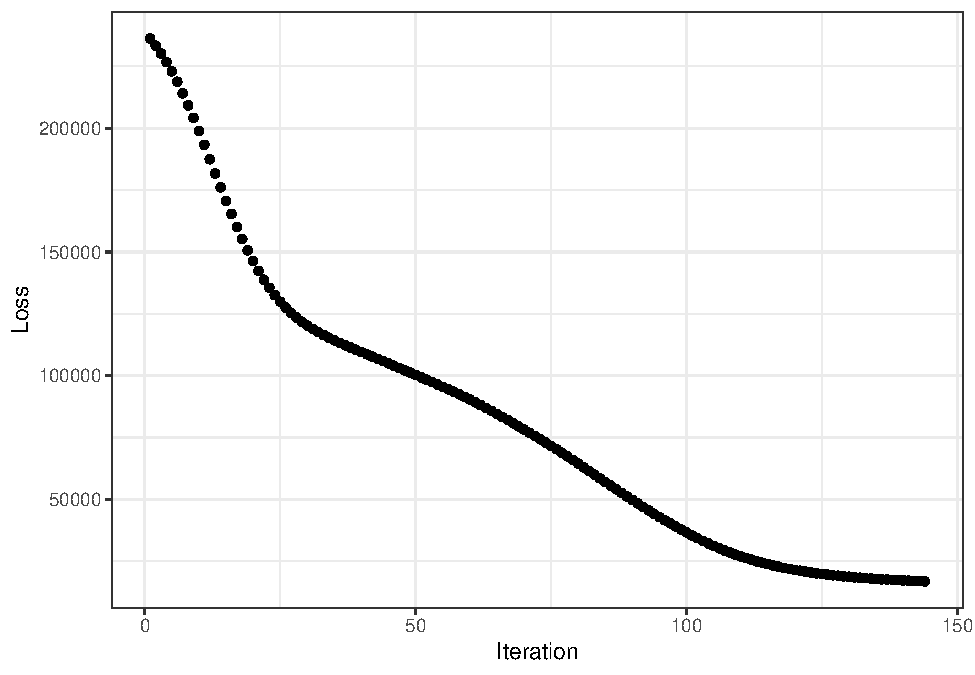
\includegraphics{_main_files/figure-latex/unnamed-chunk-35-1.pdf}

\hypertarget{other}{%
\subsection{Other}\label{other}}

\begin{Shaded}
\begin{Highlighting}[]
\DocumentationTok{\#\# get\_layer\_size function}
\NormalTok{get\_layer\_sizes }\OtherTok{\textless{}{-}} \ControlFlowTok{function}\NormalTok{(NN\_obj) \{}
\NormalTok{  n\_1 }\OtherTok{\textless{}{-}} \FunctionTok{ncol}\NormalTok{(NN\_obj}\SpecialCharTok{$}\NormalTok{W[[}\DecValTok{2}\NormalTok{]])}
  
\NormalTok{  n\_H }\OtherTok{\textless{}{-}} \FunctionTok{sapply}\NormalTok{(NN\_obj}\SpecialCharTok{$}\NormalTok{W[}\SpecialCharTok{{-}}\DecValTok{1}\NormalTok{],}
\NormalTok{                nrow)}
  
  \FunctionTok{return}\NormalTok{(}\FunctionTok{c}\NormalTok{(n\_1, n\_H))}
\NormalTok{\}}
\end{Highlighting}
\end{Shaded}

\begin{Shaded}
\begin{Highlighting}[]
\NormalTok{layer\_sizes\_test }\OtherTok{\textless{}{-}} \FunctionTok{get\_layer\_sizes}\NormalTok{(final\_NN)}
\end{Highlighting}
\end{Shaded}

\begin{center}\rule{0.5\linewidth}{0.5pt}\end{center}

\hypertarget{next-steps}{%
\section{Next Steps}\label{next-steps}}

In the future:

\begin{itemize}
\tightlist
\item
  need some sort of divergence check / pick `best so far' output
\item
  vis for gradient descent --- pick 2 vars and for every combo of those 2, plot the objective function
\item
  vis for gradient descent --- show the evolution of the var through gradient descent over iterations
\item
  NN overall vis \& perhaps animation
\item
  multi-dimensional output (cat / 1-hot)
\item
  different cost functions (softmax squared-error \& cross-entropy)
\item
  `from scratch' from scratch --- mmult and maybe further lol
\item
  get `best-case' / perfect objective function (if data creation process known)
\item
  stochastic gradient descent, minibatches (what gets passed down to GD\_iter from GD\_perform)
\item
  regularization methods \& CV-validation
\end{itemize}

\begin{center}\rule{0.5\linewidth}{0.5pt}\end{center}

\end{document}
